% Konfiguration
% config
\documentclass[parskip=half,ngerman,paper=a4,abstract,fontsize=11pt,numbers=noendperiod,bibliography=totocnumbered,listof=totoc]{scrreprt}
\usepackage{scrpage2}
\automark[chapter]{section}

% pdf
\pdfminorversion=4

% Fussnoten in Tabellen
\usepackage{threeparttable}

% table of content configuration
\setcounter{secnumdepth}{2}
\setcounter{tocdepth}{2}

% heading for appendix
\clearscrheadfoot
\cfoot{\pagemark}
\ohead{\textnormal{\textbf{\headmark}}}


\ohead{\small{Jennifer Wozniak, 10004257}}
%\usepackage{scrpage2}
\pagestyle{scrheadings}





% layout
\usepackage[left=4cm,right=2cm,top=1.5cm,bottom=2.5cm,includeheadfoot,headheight=1.3\baselineskip]{geometry}
\renewcommand{\chapterpagestyle}{scrheadings}
\renewcommand*{\chapterheadstartvskip}{\vspace*{-0.5\baselineskip}}
% footnote
\usepackage{remreset}
\makeatletter\@removefromreset{footnote}{chapter}\makeatother

\usepackage{lmodern}
\usepackage{babel}
\usepackage[utf8]{inputenc}
\usepackage[babel,german=quotes]{csquotes}

% 1,5 line space
\usepackage{setspace}
\onehalfspacing

% landscape sites
\usepackage{lscape}

% pictures
\usepackage{graphicx}
\newcommand{\includegraphix}[2]{\IfFileExists{#1}{\includegraphics[#2]{#1}}{\includegraphics[draft,#2]{#1}}}
\usepackage{placeins}
\usepackage{wrapfig}
\usepackage{rotating}

% bibliography
\usepackage[style=alphabetic-verb,block=space,backend=biber,bibencoding=utf8]{biblatex}
\bibliography{library/bibliography}

\defbibheading{Literatur}{\section{Literatur}}
\defbibheading{Internet}{\section{Internet}}

% links
\usepackage[pdfborder={0 0 0}, unicode=true]{hyperref}
\usepackage{pdfsync}

% floatingareas
\let\mysection=\section
\renewcommand{\section}[1]{\FloatBarrier\mysection{#1}}

\let\mysubsection=\subsection
\renewcommand{\subsection}[1]{\FloatBarrier\mysubsection{#1}}

\let\mysubsubsection=\subsubsection
\renewcommand{\subsubsection}[1]{\FloatBarrier\mysubsubsection{#1}}

\let\myparagraph=\paragraph
\renewcommand{\paragraph}[1]{\FloatBarrier\myparagraph{#1}}

\let\mysubparagraph=\subparagraph
\renewcommand{\subparagraph}[1]{\FloatBarrier\mysubparagraph{#1}}

\usepackage{float}

% glossaries
\usepackage[acronym,nopostdot]{glossaries}
\renewcommand{\acronymname}{Abkürzungsverzeichnis}
\renewcommand*{\glssettoctitle}[1]{\def\glossarytoctitle{\csname @glotype@#1@title\endcsname}}

\let\mygls=\gls
\renewcommand{\gls}[1]{\protect\glsIfListOfAcronyms{\glsentrytype{#1}}{\textnormal{\textit{\mygls{#1}}}}{\textnormal{\textbf{\mygls{#1}\footnote{siehe Glossar: \mygls{#1}}}}}}
\newcommand{\glsLink}[1]{\mygls{#1}}

\let\myglspl=\glspl
\renewcommand{\glspl}[1]{\protect\glsIfListOfAcronyms{\glsentrytype{#1}}{\textnormal{\textit{\myglspl{#1}}}}{\textnormal{\textbf{\myglspl{#1}\footnote{siehe Glossar: \mygls{#1}}}}}}

\let\myglsfirst=\glsfirst
\renewcommand{\glsfirst}[1]{\protect\glsIfListOfAcronyms{\glsentrytype{#1}}{\textnormal{\textit{\myglsfirst{#1}}}}{\textnormal{\textbf{\myglsfirst{#1}\footnote{siehe Glossar: \mygls{#1}}}}}}

\let\myglsdisp=\glsdisp
\renewcommand{\glsdisp}[2]{\protect\glsIfListOfAcronyms{\glsentrytype{#1}}{\textnormal{\textit{\myglsdisp{#1}{#2}}}}{\textnormal{\textbf{\myglsdisp{#1}{#2}\footnote{siehe Glossar: \mygls{#1}}}}}}

\newglossarystyle{myListStyle}{\setglossarystyle{list}\renewcommand*{\glossaryentryfield}[5]{\item[\glstarget{##1}{##2}]##3\glspostdescription\dotfill\space{##5}}}

\makeatletter
\renewcommand*\dotfill{\leavevmode%
	\leaders\hbox{$\m@th \mkern \@dotsep mu\hbox{.}\mkern \@dotsep mu$}\hfill\kern\z@}
\makeatother

% todos
\usepackage{todonotes}
\reversemarginpar

\usepackage{color}
\definecolor{todo}{rgb}{1,.7,.6}
\definecolor{comment}{rgb}{1,1,.8}
\definecolor{correction}{rgb}{.7,1,.7}

\let\mytodo=\todo
\renewcommand{\todo}[1]{\protect\mytodo[fancyline, backgroundcolor=todo, size=\footnotesize]{TODO:\\#1}}
\newcommand{\TODO}[1]{\protect\mytodo[fancyline, backgroundcolor=todo, size=\footnotesize]{TODO:\\#1}}
\newcommand{\comment}[1]{\protect\mytodo[fancyline, backgroundcolor=comment, size=\footnotesize]{Comment:\\#1}}
\newcommand{\correction}[1]{\protect\mytodo[fancyline, backgroundcolor=correction, size=\footnotesize]{Correction:\\#1}}
 
% zitate
\let\mycite = \cite
\renewcommand{\cite}[1]{\footnote{\mycite{#1}}}
\newcommand{\ccite}[1]{\footnote{Vgl. \mycite{#1}}}

% Grafiken auf der Titelseite
\usepackage{subfigure}
\usepackage[font=small]{caption} % Bei zu wenig Text das hier wieder rausnehmen

%listings
\usepackage{listings}
%\renewcommand{\lstlistingname}{Beispiel}
\lstset{breaklines=true,captionpos=b,title=\lstname}

%custom enumerate 
\usepackage{enumitem}

%math symbols
\usepackage {amsmath}
\usepackage{amssymb}
\usepackage{amstext}
\usepackage{amsfonts}
\usepackage{mathrsfs}
\usepackage{nicefrac}
\usepackage{amsthm}
\newtheorem{mydef}{Definition}
\newtheorem{example}{Beispiel}
%Eigene Befehle:
\newcommand{\x}{\cdot}
%flowchart
\usepackage{tikz}
\usetikzlibrary{shapes.geometric, arrows}
\tikzstyle{startstop} = [rectangle, rounded corners, minimum width=3cm, minimum height=1cm, text centered, draw=black, fill=red!30]
\tikzstyle{io} = [trapezium, trapezium left angle=70, trapezium right angle=110, text width=5.2cm, minimum height=1cm, text centered, draw=black, fill=blue!30]
\tikzstyle{process} = [rectangle,text width=6cm, minimum height=1cm, text centered, draw=black, fill=orange!30]
\tikzstyle{decision} = [diamond, minimum width=3cm, minimum height=1cm, text centered, draw=black, fill=green!30]
\tikzstyle{arrow} = [thick,->,>=stealth]

%url
\usepackage{url}

% MakeIndex NICHT NÖTIG
%\usepackage{makeidx}
\makeindex

% Glossar
%Abkürzungen
\newglossaryentry{abk:abk}{
	type=\acronymtype,
	name={Abk},
	first={Abkürzung (Abk)},
	description={Abkürzung}
}




%Glossareintrag
\newglossaryentry{glo:glossareintrag}{
	name={Glossareintrag},
	description={Ein beispielhafter Glossareintrag mit einer ausführlichen Beschreibung.}
}
\makeglossaries

% Dokumenteneinsellungen
\newcommand{\documentDate}{\today}
\newcommand{\documentAuthorA}{Jennifer Wozniak}
\newcommand{\documentAuthorMatricleNumberA}{Matrikelnummer: 10004257}
\newcommand{\documentAuthorStreetA}{Schaufelder Straße 33A}
\newcommand{\documentAuthorPostalcodeA}{30167}
\newcommand{\documentAuthorCityA}{Hannover}
\newcommand{\documentUniCourse}{B.Sc. Maschinenbau}
\newcommand{\documentTitle}{Konstruktives Projekt 4}

\DeclareCaptionType{code}[Quelltext][Quelltextverzeichnis] 

% Beginn Hauptdokument
\begin{document}
	% Seitennummerierung alphabetisch (nur für das PDF Inhaltsverzeichnis notwendig)
	\pagenumbering{alph}
	\setcounter{page}{1}
	
	% Titelseite
	% titlepage

\begin{titlepage}


\begin{center}
\sffamily{
\rule{\linewidth}{0.2mm} 	\\[0.3cm]
\normalsize
\huge{\textbf{ \documentTitle}}\\
\rule{\linewidth}{0.2mm} 	\\[1cm]


\vspace{1cm}

\normalsize{Verfasser:\\}\Large{\documentAuthorA \\ \documentAuthorMatricleNumberA\\ \documentAuthorStreetA \\ \documentAuthorPostalcodeA\space\documentAuthorCityA}\\



\vspace{1cm}


\normalsize{Studiengang:\\}\Large{\documentUniCourse}\\

\vspace{1cm}

\normalsize
Eingereicht am:\\
\Large{\documentDate}}

\end{center}


\normalsize
\vfill
\end{titlepage}
	%Sperrvermerk
	%\include{document/sperrvermerk}
	% Zusammenfassung (Abstract)
	%\include{content/abstract}
	
	% Seitennummerierung römisch
	\pagenumbering{Roman}
	\setcounter{page}{1}
	
	
	% Inhaltsverzeichnis
	\clearpage\phantomsection\pdfbookmark{\contentsname}{toc}
	\tableofcontents
	\newpage
	
	
	
	% Seitennummerierung arabisch
	\pagenumbering{arabic}
	\setcounter{page}{1}
	
	% Inhalt Start
	\chapter{Anforderungsliste}
\mbox{} \begin{center}
	\begin{sideways}%[htbp]
		\vspace{-1cm}
		\begin{minipage}{1.3\textwidth}
			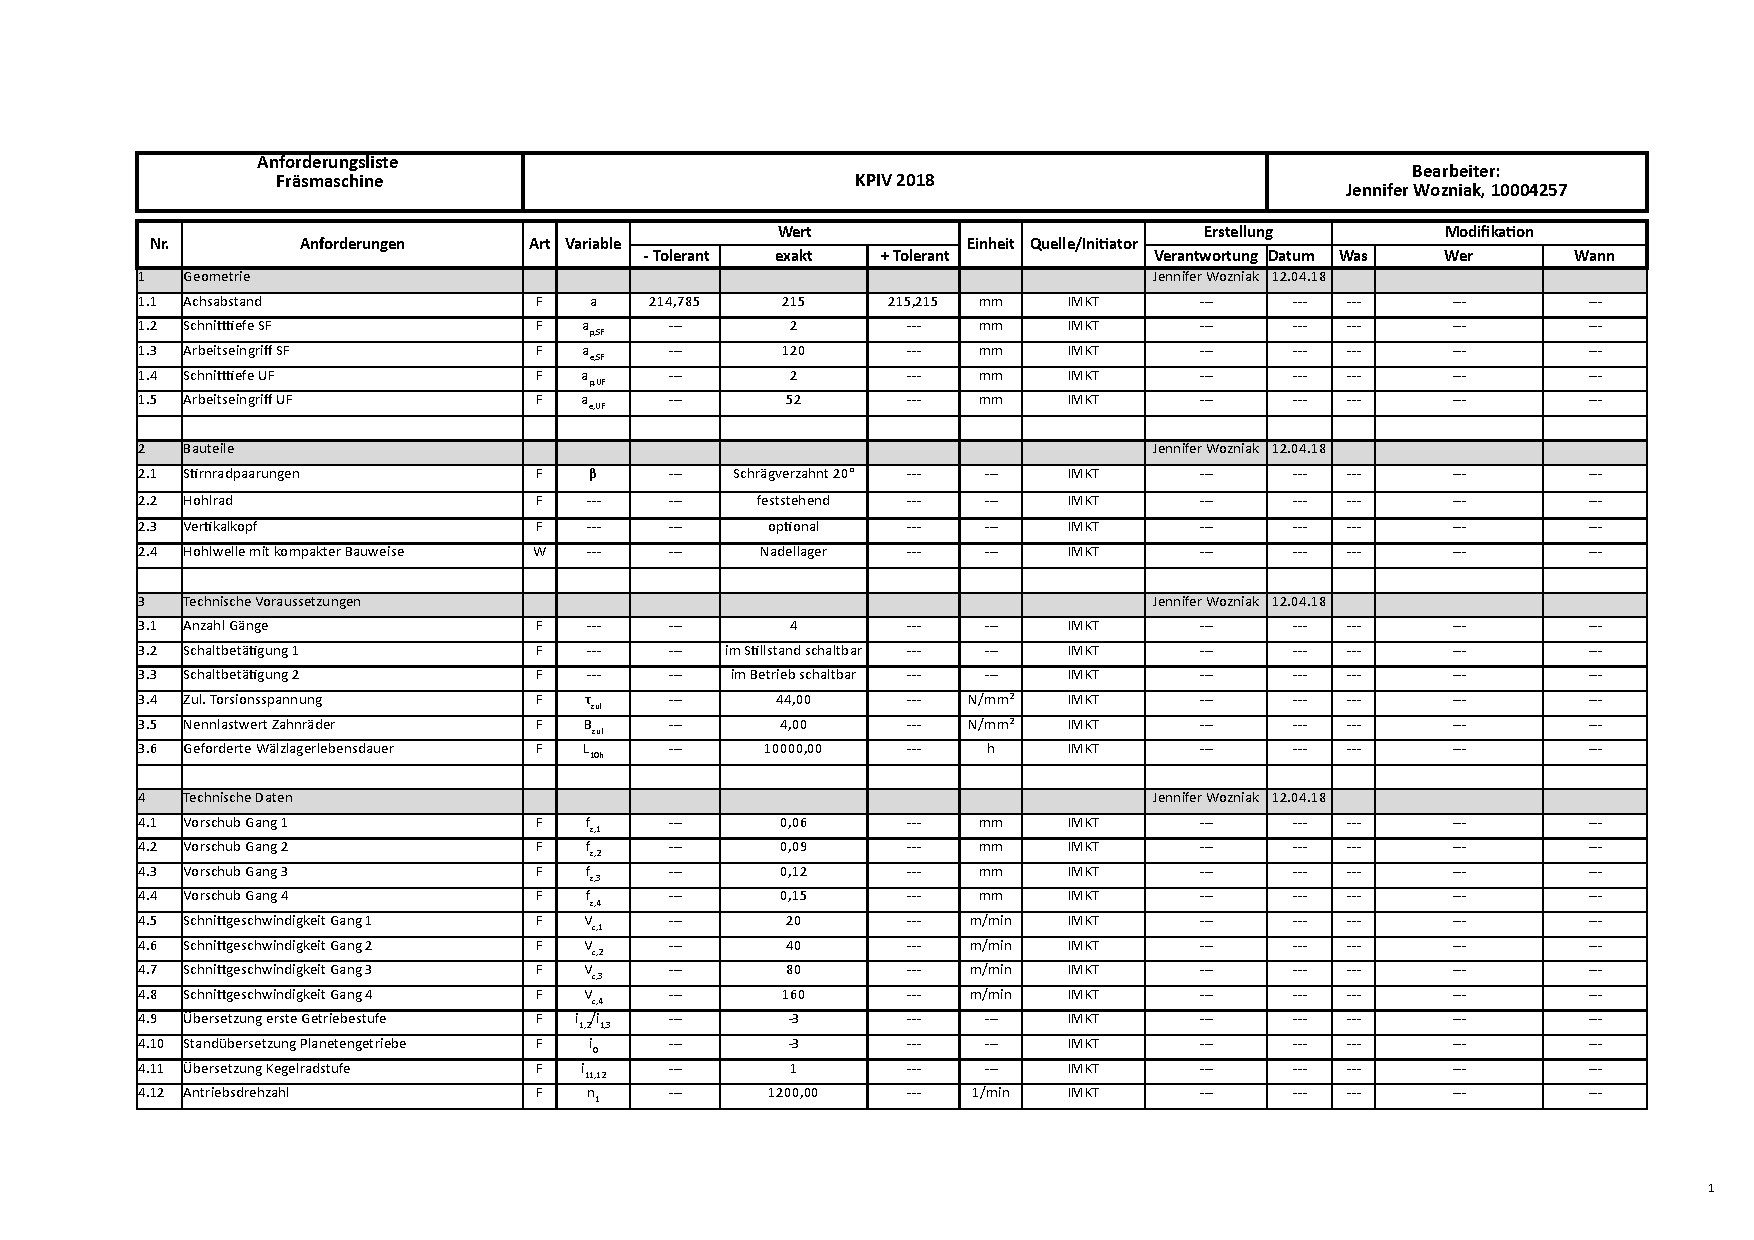
\includegraphics[width=1.04\textwidth,keepaspectratio]{figures/Anforderungsliste.pdf}
			\label{fig:anforderungsliste}
		\end{minipage}
	\end{sideways}
\end{center}
%\vspace*{-2cm}
%\begin{sidewaysfigure}
%	\centering
%	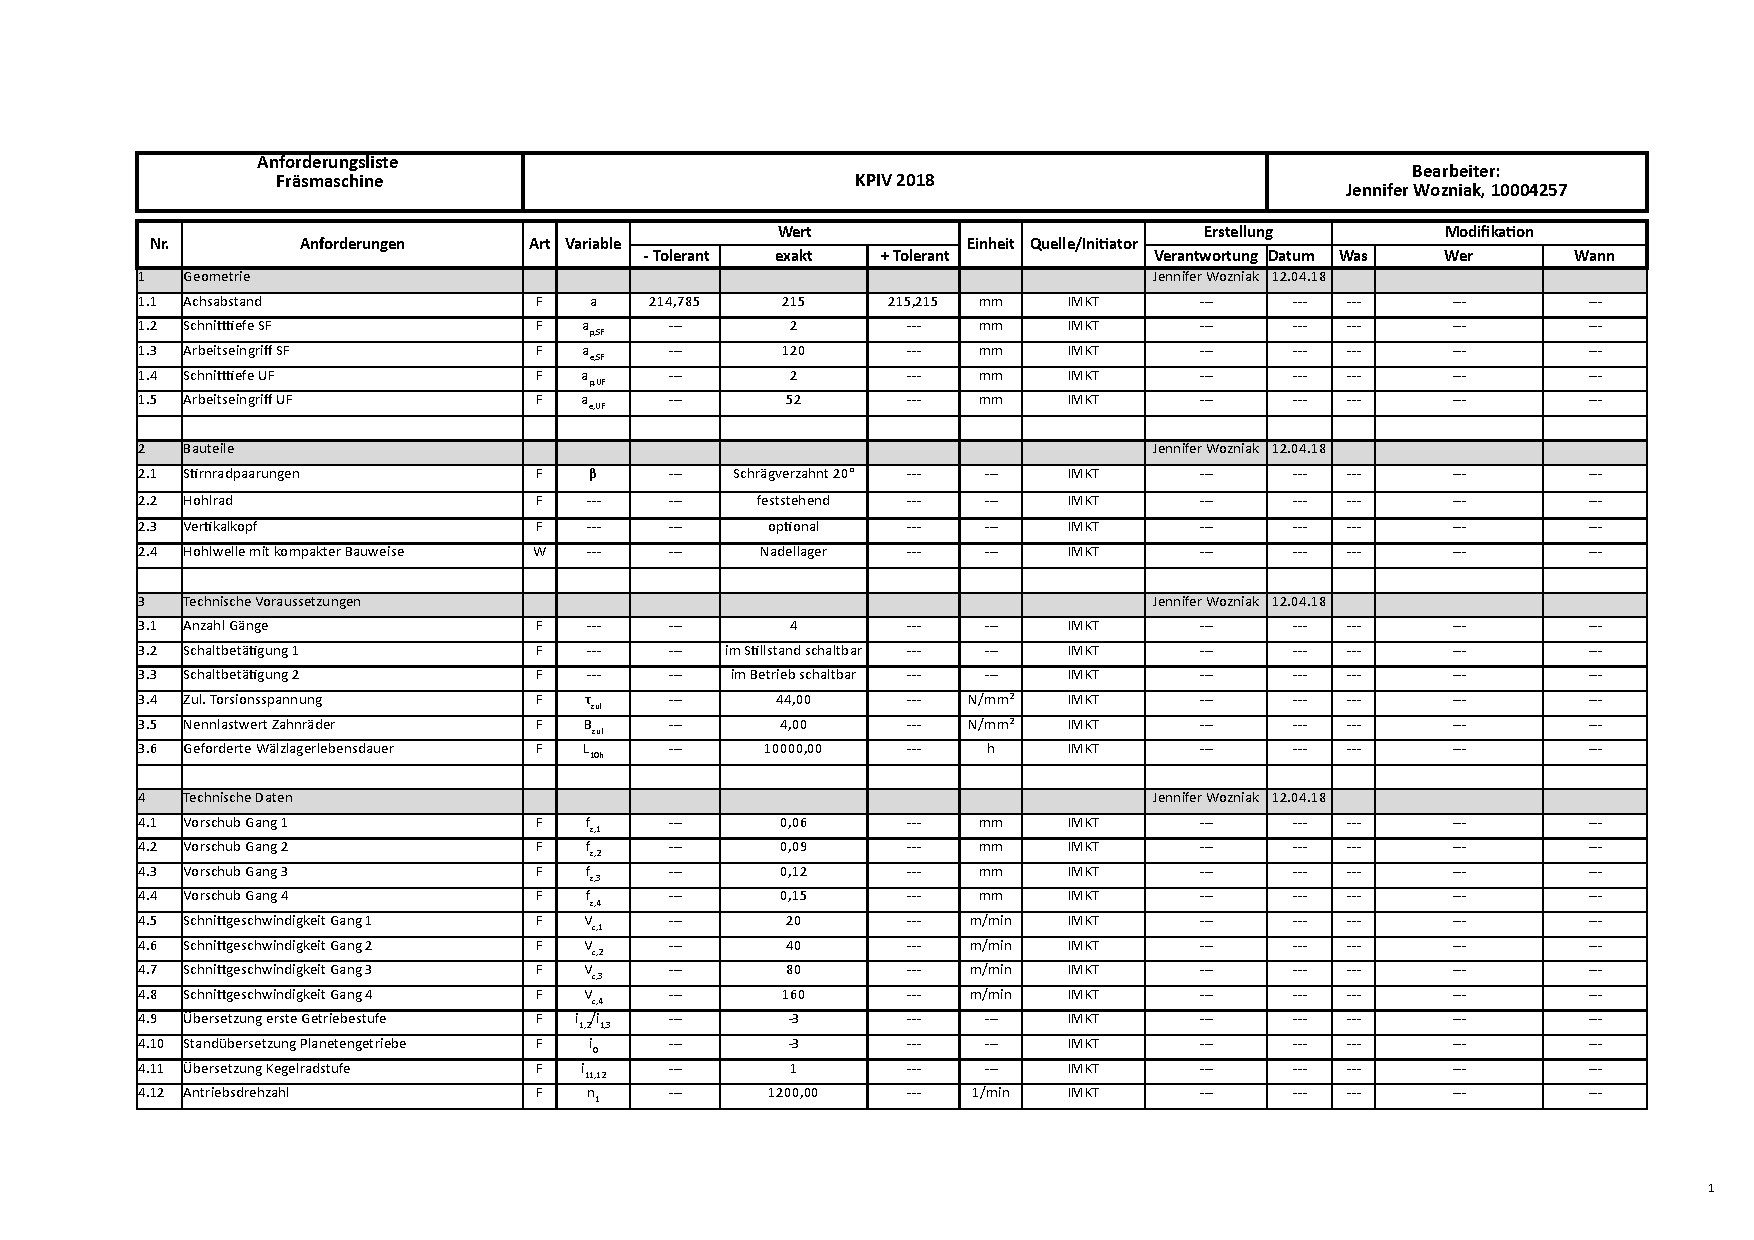
\includegraphics[width=1\textwidth, height=.8\textheight]{figures/Anforderungsliste.pdf}
%	\label{fig:anforderungsliste}
%\end{sidewaysfigure}
%\centering{\rotatebox{90}{
%	\begin{minipage}{1\textheight}
%		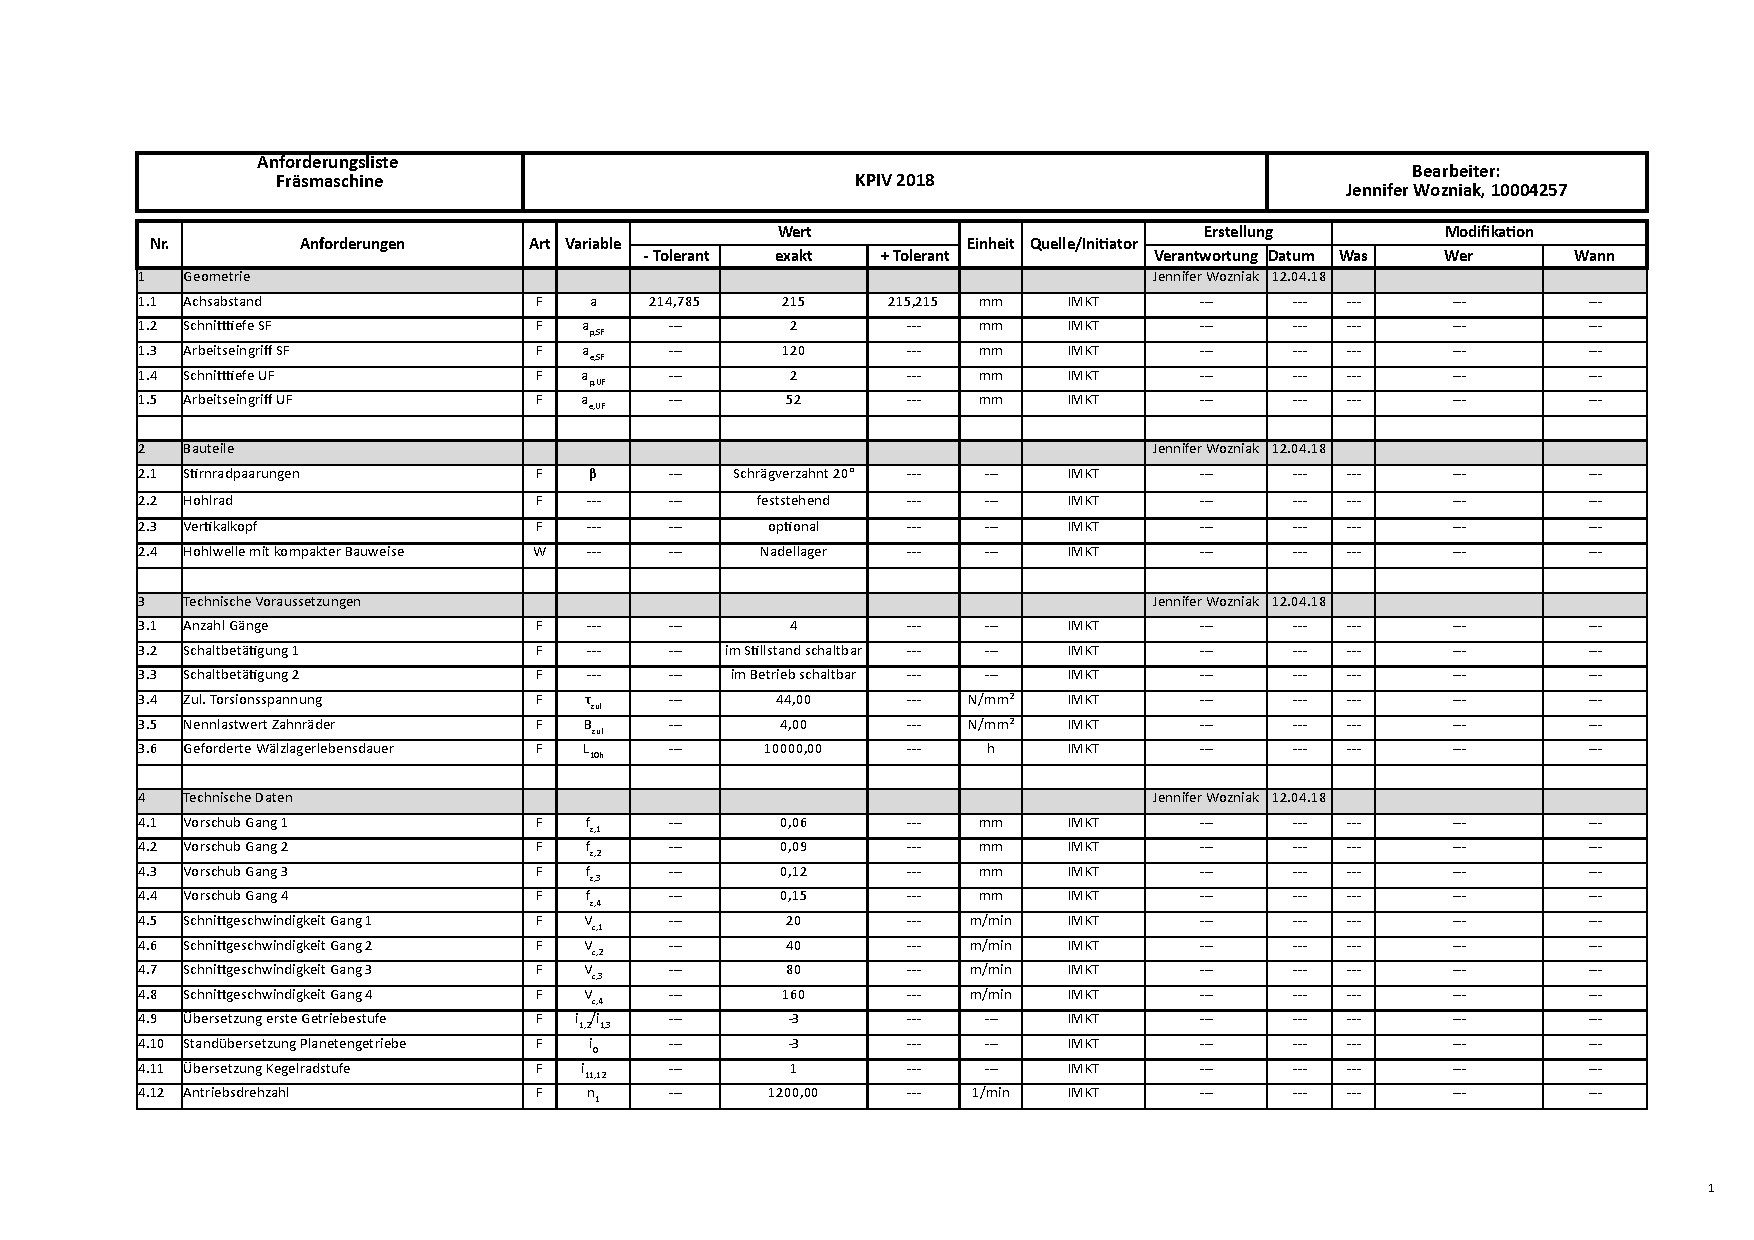
\includegraphics[width=1\textwidth]{figures/Anforderungsliste.pdf}
%		%\caption[Anforderungsliste]{Anforderungsliste}
%		\label{fig:anforderungsliste}
%	\end{minipage}
%}
%}

	\chapter{Vorauslegung}
\pagestyle{scrheadings}
	\section{Übersetzungen und Drehzahlen}
\subsubsection{Festlegen der Gänge: }
\begin{align*}
\text{Gang 1: }& Z1/Z2 \text{ und } Z6/Z7 \\
\text{Gang 2: }& Z1/Z2 \text{ und } Z4/Z5 \\
\text{Gang 3: }& Z1/Z3 \text{ und } Z6/Z7 \\
\text{Gang 4: }& Z1/Z3 \text{ und } Z4/Z5 \\
\end{align*}
\subsubsection{Gegeben: }
\begin{center}
\[
	v_{c,1} = 20 \frac{\text{m}}{\text{min}} \text{ , } v_{c,2} = 40 \frac{\text{m}}{\text{min}} \text{ , } v_{c,3} = 80 \frac{\text{m}}{\text{min}} \text{ , } v_{c,4} = 160 \frac{\text{m}}{\text{min}}
\]
\[
	D_{WZ,U} = 120 \text{mm; }
	D_{WZ,S} = 120 \text{mm }
\]
\[
	n_{an} = n_{\mathord{\mathrm{I}}}= 1200 \frac{1}{\text{min}}
\]
\[
	i_{1,2} =  i_{1,3} = -3
\]
 \begin{align*}
\text{Planetengetriebe: }
		&i_{0} = -3 \\	
		&n_{10} = 0\\
\end{align*}
\subsubsection{Berechnungen:}
\end{center}
Verwendete Formeln aus den Skripten KL II\ccite{bib:denkena:kl2} S. 34 und KL III\ccite{bib:poll:kl3} S. 2 \\
Mithilfe der Schnittgeschwindigkeiten werden die Abtriebsdrehzahlen der einzelnen Gänge bestimmt. Anschließend können dann die fehlenden Übersetzungen ermittelt werden.
\begin{itemize}
\item{Gang 1:}
\begin{align*}
	&n_{{\mathord{\mathrm{II}},1}} = \frac{n_{an}}{i_{1,2}} = 400 \frac{1}{\text{min}} \\
	&\text{Formel nach Willis: } n_{9}= \frac{n_8 - i_0 \x n_{10}}{1-i_0}\\
	&n_{9,1}= n_{\mathord{\mathrm{III}},1} = \frac{n_{8,1}}{1-i_0} = \frac{400 \frac{1}{\text{min}}}{1-(-3)} = 100 \frac{1}{\text{min}}\\
	&n_{\mathord{\mathrm{IV}},1} = n_{ab,1} =\frac{ v_{c,1}}{\pi \x D_{WZ}} = 53,05 \frac{1}{\text{min}} \\
	&\implies i_{6,7} = \frac{n_{{\mathord{\mathrm{III}},1}}}{n_{\mathord{\mathrm{IV}},1}} = -1,89 \\
\end{align*}
\item{Gang 2:}
\begin{align*}
	&n_{{\mathord{\mathrm{II}},2}} = \frac{n_{an}}{i_{1,2}} = 400 \frac{1}{\text{min}} \\
	&n_{\mathord{\mathrm{IV}},2} =n_{ab,2} = \frac{ v_{c,2}}{\pi \x D_{WZ}} =106,1 \frac{1}{\text{min}} \\
	&\implies i_{4,5} = \frac{ n_{\mathord{\mathrm{III}},2}}{n_{\mathord{\mathrm{IV}},2}} = 3,77 \\
\end{align*}
\item{Gang 3:}
\begin{align*}
		&n_{\mathord{\mathrm{III}},3} = \frac{n_{an}}{i_{1,3}} = 400 \frac{1}{\text{min}} \\
		&n_{\mathord{\mathrm{IV}},3} =\frac{ n_{\mathord{\mathrm{III}},3}}{i_{6,7}} =212,2 \frac{1}{\text{min}}\\	
		&\text{Überprüfung der Abtriebsdrehzahl: } n_{\mathord{\mathrm{IV}},3} =n_{ab,3} = \frac{ v_{c,3}}{\pi \x D_{WZ}} =212,2 \frac{1}{\text{min}} \\
\end{align*}
\item{Gang 4:}
\begin{align*}
	&n_{\mathord{\mathrm{III}},4} = n_{9,4}= \frac{n_{an}}{i_{1,3}} = 400 \frac{1}{\text{min}} \\
	&\text{Formel nach Willis: } n_{8}= i_0 \x n_{10} + n_9\x (1-i_0) \\
	&n_{8,4}= n_{\mathord{\mathrm{II}},4} = n_{9,4}\x (1-i_0) = 400 \frac{1}{\text{min}} \x (1- (-3)) = 1600 \frac{1}{\text{min}}\\
	&n_{\mathord{\mathrm{IV}},4} =\frac{ n_{\mathord{\mathrm{II}},4}}{i_{4,5}} =424,4 \frac{1}{\text{min}}\\
	&\text{Überprüfung der Abtriebsdrehzahl: } n_{\mathord{\mathrm{IV}},4} =n_{ab,4} = \frac{ v_{c,4}}{\pi \x D_{WZ}} =424,4 \frac{1}{\text{min}} \\
\end{align*}
\end{itemize}
	\section{Torsionsmomente \& Mindestdurchmesser}
Um die wirkenden Torsionsmomente zu bestimmen, wird zunächst die benötigte Schnittleistung für das Umfangs- sowie das Stirnfräsen berechnet. Die verwendeten Formeln stammen aus dem Aufgabenblatt, welches vom IMKT ausgehändigt wurde.
\subsubsection{Schnittleistung:}
\begin{itemize}
\item{Umfangsfräsen:}
\begin{align*}
	&\textbf{gegeben: } \\
	&D_{WZ,U} = 120 \text{ mm, } a_e = 52 \text{ mm } \implies u_{U} = \frac{D_{WZ,U}}{2} - a_e = 8 \text{ mm} \\
	&z= 12 \text{ , } a_p=b=2\text{ mm, }\kappa = 90^\circ \\
	&f_{z,1} = 0,06 \text{ mm, } f_{z,2} = 0,09 \text{ mm, } f_{z,3} = 0,12 \text{ mm, } f_{z,4} = 0,15 \text{ mm } \\
	&\textbf{Rechnung: } \\
	&\varphi_s = \arccos \left( 1-  \frac{2\x (u_{U} + a_e)}{D_{WZ,U}} \right) - \arccos \left( 1-  \frac{2\x u_{U}}{D_{WZ,U}} \right) = 60,07 ^\circ \\
	&z_{iE} = \text{RUNDEN}\left( \frac{\varphi \x z}{360 ^\circ} \right) = 2 \\
	&h_m = \frac{114,6 ^\circ}{\varphi_s} \x f_z \x \frac{a_e}{D_{WZ,U}} \x \sin (\kappa ) \\
	&h_{m,1} = \frac{114,6 ^\circ}{60,07 ^\circ} \x 0,06 \text{ mm} \x \frac{52\text{ mm}}{120 \text{ mm}} \x \sin (90 ^\circ )  =  0,05 \text{ mm} \\
	&h_{m,2} = 0,074 \text{ mm} \\
	&h_{m,3} = 0,099 \text{ mm} \\
	&h_{m,4} = 0,12 \text{ mm} \\
	&F_{cz} = b \x h_m ^{1-z} \x k_{c1.1} \x K_{V,c}\\
	&F_{cz,1} = 2 \text{ mm } \x 0,05 \text{ mm } ^{0,7}  \x 2500 \frac{\text{N}}{\text{mm} ^2} \x 1,7= 926,1 \text{ N} \\
	&F_{cz,2} = 1237,8 \text{ N} \\
	&F_{cz,3} = 1535,3 \text{ N} \\
	&F_{cz,4} = 1770,2 \text{ N} \\
	&\implies P_c = z_{iE} \x v_c \x F_{cz} \\
	&P_{c,1} = 2 \x 0,34 \frac{\text{m}}{\text{s}} \x 926,1 \text{ N} = 629,75 \text{ W} \\
	&P_{c,2} = 1658,7 \text{ W} \\
	&P_{c,3} = 4114,6 \text{ W} \\
	&P_{c,4} = 9452,87 \text{ W} \\
\end{align*}
\item{Stirnfräsen:}
\begin{align*}
	&\textbf{gegeben: } \\
	&D_{WZ,S} = 120 \text{ mm, } a_e = 120 \text{ mm } \implies u_{S} = \frac{D_{WZ,S}}{2} - a_e = 0 \text{ mm} \\
	&z= 6 \text{ , } a_p=b=2\text{ mm, } \kappa = 90^\circ\\
	&f_{z,1} = 0,06 \text{ mm, } f_{z,2} = 0,09 \text{ mm, } f_{z,3} = 0,12 \text{ mm, } f_{z,4} = 0,15 \text{ mm } \\
	&\textbf{Rechnung: } \\
	&\varphi_s = \arccos \left( 1-  \frac{2\x (u_{S} + a_e)}{D_{WZ,S}} \right) - \arccos \left( 1-  \frac{2\x u_{S}}{D_{WZ,S}} \right) =180 ^\circ \\
	&z_{iE} = \text{RUNDEN}\left( \frac{\varphi \x z}{360 ^\circ} \right) = 3 \\
	&h_m = \frac{114,6 ^\circ}{\varphi_s} \x f_z \x \frac{a_e}{D_{WZ,S}} \x \sin (\kappa ) \\
	&h_{m,1} = \frac{114,6 ^\circ}{180 ^\circ} \x 0,06 \text{ mm} \x \frac{120\text{ mm}}{120 \text{ mm}} \x \sin (90 ^\circ )  =  0,038 \text{ mm} \\
	&h_{m,2} = 0,057 \text{ mm} \\
	&h_{m,3} = 0,0764 \text{ mm} \\
	&h_{m,4} = 0,0955 \text{ mm} \\
	&F_{cz} = b \x h_m ^{1-z} \x k_{c1.1} \x K_{V,c}\\
	&F_{cz,1} = 2 \text{ mm } \x 0,038 \text{ mm } ^{0,7}  \x 2500 \frac{\text{N}}{\text{mm} ^2} \x 1,7= 755,9 \text{ N} \\
	&F_{cz,2} = 1020,39 \text{ N} \\
	&F_{cz,3} = 1267,38 \text{ N} \\
	&F_{cz,4} = 1494,93 \text{ N} \\
	&\implies P_c = z_{iE} \x v_c \x F_{cz} \\
	&P_{c,1} = 3 \x 0,34 \frac{\text{m}}{\text{s}} \x 755,9 \text{ N} = 771,02 \text{ W} \\
	&P_{c,2} = 2050,98 \text{ W} \\
	&P_{c,3} = 5094,87 \text{ W} \\
	&P_{c,4} = 11974,39 \text{ W} \\
\end{align*}
\end{itemize}
\subsubsection{Torsionsmomente:}
Die verwendete Formel zur Berechnung der Torsionsmomente stammt aus dem Skript zur Konstruktionslehre III\ccite{bib:poll:kl3} Seite 2.
\[
	T=\frac{P}{2 \pi \x n}
\]
\begin{itemize}
\item {Umfangsfräsen: }
\begin{align*}
	&\textbf{Gang 1: } \\
	&T_{\mathord{\mathrm{I}},1,U} = \frac{P_{c,1,U}}{2 \pi \x n_{an}} = \frac{629,75 \text{ W} }{2 \pi \x 1200 \frac{1}{\text{min}}} = 5 \text{ Nm} \\
	&T_{\mathord{\mathrm{II}},1,U} = \frac{P_{c,1,U}}{2 \pi \x n_{\mathord{\mathrm{II}},1}} = \frac{629,75 \text{ W} }{2 \pi \x 400 \frac{1}{\text{min}}} = 15 \text{ Nm} \\
	&T_{\mathord{\mathrm{III}},1,U} = \frac{P_{c,1,U}}{2 \pi \x n_{\mathord{\mathrm{III}},1}} = \frac{629,75 \text{ W} }{2 \pi \x 100 \frac{1}{\text{min}}} = 60,14 \text{ Nm} \\
	&T_{\mathord{\mathrm{IV}},1,U} = \frac{P_{c,1,U}}{2 \pi \x n_{\mathord{\mathrm{IV}},1}} = \frac{629,75 \text{ W} }{2 \pi \x 53,05 \frac{1}{\text{min}}} =112,36 \text{ Nm} \\
	&\textbf{Gang 2: } \\
	&T_{\mathord{\mathrm{I}},2,U} = \frac{P_{c,2,U}}{2 \pi \x n_{an}} = \frac{1658,7 \text{ W} }{2 \pi \x 1200 \frac{1}{\text{min}}} = 13,2 \text{ Nm} \\
	&T_{\mathord{\mathrm{II}},2,U} = \frac{P_{c,2,U}}{2 \pi \x n_{\mathord{\mathrm{II}},2}} = 39,6 \text{ Nm} \\
	&T_{\mathord{\mathrm{IV}},2,U} = \frac{P_{c,2,U}}{2 \pi \x n_{\mathord{\mathrm{IV}},2}} = 149,29 \text{ Nm} \\
	&\textbf{Gang 3: } \\
	&T_{\mathord{\mathrm{I}},3,U} = \frac{P_{c,3,U}}{2 \pi \x n_{an}} = \frac{4114,6 \text{ W} }{2 \pi \x 1200 \frac{1}{\text{min}}} = 32,74 \text{ Nm} \\
	&T_{\mathord{\mathrm{III}},3,U} = \frac{P_{c,3,U}}{2 \pi \x n_{\mathord{\mathrm{III}},3}} = 98,23 \text{ Nm} \\
	&T_{\mathord{\mathrm{IV}},3,U} = \frac{P_{c,3,U}}{2 \pi \x n_{\mathord{\mathrm{IV}},3}} = 185,16 \text{ Nm} \\
	&\textbf{Gang 4: } \\
	&T_{\mathord{\mathrm{I}},4,U} = \frac{P_{c,4,U}}{2 \pi \x n_{an}} = \frac{9452,87 \text{ W} }{2 \pi \x 1200 \frac{1}{\text{min}}} =75,22 \text{ Nm} \\
	&T_{\mathord{\mathrm{II}},4,U} = \frac{P_{c,4,U}}{2 \pi \x n_{\mathord{\mathrm{II}},4}} =56,42 \text{ Nm} \\
	&T_{\mathord{\mathrm{III}},4,U} = \frac{P_{c,4,U}}{2 \pi \x n_{\mathord{\mathrm{III}},4}} = 225,67 \text{ Nm} \\
	&T_{\mathord{\mathrm{IV}},4,U} = \frac{P_{c,4,U}}{2 \pi \x n_{\mathord{\mathrm{IV}},4}} =212,35 \text{ Nm} \\
\end{align*}	
\item {Stirnfräsen: }
\begin{align*}
	&\textbf{Gang 1: } \\
	&T_{\mathord{\mathrm{I}},1,S} = \frac{P_{c,1,S}}{2 \pi \x n_{an}} = \frac{771,02 \text{ W} }{2 \pi \x 1200 \frac{1}{\text{min}}} = 6,12 \text{ Nm} \\
	&T_{\mathord{\mathrm{II}},1,S} = \frac{P_{c,1,S}}{2 \pi \x n_{\mathord{\mathrm{II}},1}} = \frac{771,02 \text{ W} }{2 \pi \x 400 \frac{1}{\text{min}}} = 18,4 \text{ Nm} \\
	&T_{\mathord{\mathrm{III}},1,S} = \frac{P_{c,1,S}}{2 \pi \x n_{\mathord{\mathrm{III}},1}} = \frac{771,02 \text{ W} }{2 \pi \x 100 \frac{1}{\text{min}}} = 73,63 \text{ Nm} \\
	&T_{\mathord{\mathrm{IV}},1,S} = \frac{P_{c,1,S}}{2 \pi \x n_{\mathord{\mathrm{IV}},1}} = \frac{771,02 \text{ W} }{2 \pi \x 53,05 \frac{1}{\text{min}}} =138,79 \text{ Nm} \\
	&\textbf{Gang 2: } \\
	&T_{\mathord{\mathrm{I}},2,S} = \frac{P_{c,2,S}}{2 \pi \x n_{an}} = \frac{2050,98 \text{ W} }{2 \pi \x 1200 \frac{1}{\text{min}}} = 16,32 \text{ Nm} \\
	&T_{\mathord{\mathrm{II}},2,S} = \frac{P_{c,2,S}}{2 \pi \x n_{\mathord{\mathrm{II}},2}} = 48,96 \text{ Nm} \\
	&T_{\mathord{\mathrm{IV}},2,S} = \frac{P_{c,2,S}}{2 \pi \x n_{\mathord{\mathrm{IV}},2}} = 184,59 \text{ Nm} \\
	&\textbf{Gang 3: } \\
	&T_{\mathord{\mathrm{I}},3,S} = \frac{P_{c,3,S}}{2 \pi \x n_{an}} = \frac{5094,87 \text{ W} }{2 \pi \x 1200 \frac{1}{\text{min}}} = 40,54 \text{ Nm} \\
	&T_{\mathord{\mathrm{III}},3,S} = \frac{P_{c,3,S}}{2 \pi \x n_{\mathord{\mathrm{III}},3}} = 121,63 \text{ Nm} \\
	&T_{\mathord{\mathrm{IV}},3,S} = \frac{P_{c,3,S}}{2 \pi \x n_{\mathord{\mathrm{IV}},3}} = 229,28 \text{ Nm} \\
	&\textbf{Gang 4: } \\
	&T_{\mathord{\mathrm{I}},4,S} = \frac{P_{c,4,S}}{2 \pi \x n_{an}} = \frac{11974,39 \text{ W} }{2 \pi \x 1200 \frac{1}{\text{min}}} =95,29 \text{ Nm} \\
	&T_{\mathord{\mathrm{II}},4,S} = \frac{P_{c,4,S}}{2 \pi \x n_{\mathord{\mathrm{II}},4}} =71,47\text{ Nm} \\
	&T_{\mathord{\mathrm{III}},4,S} = \frac{P_{c,4,S}}{2 \pi \x n_{\mathord{\mathrm{III}},4}} = 285,87 \text{ Nm} \\
	&T_{\mathord{\mathrm{IV}},4,S} = \frac{P_{c,4,S}}{2 \pi \x n_{\mathord{\mathrm{IV}},4}} =268,99 \text{ Nm} \\
\end{align*}	
\end{itemize}
Auf jeden Welle wirken im vierten Gang beim Stirnfräsen die höchsten Torsionsmomente. Im Folgenden wird das Getriebe deshalb auf Basis dieser Momente ausgelegt.
\newpage
\subsubsection{Mindestdurchmesser:}
Mithilfe der berechneten Torsionsmomente kann nun auf die Mindestdurchmesser der jeweiligen Wellen geschlossen werden. Die verwendeten Formeln stammen aus dem Skript zur Konstruktionslehre III\ccite{bib:poll:kl3} Seiten 150 - 153 und dem Roloff/Matek\ccite{bib:roloffMatek:maschinenelemente} Seite 391
\begin{align*}
	&\tau_t = \frac{M}{W_p} \implies W_p = \frac{M}{\tau_{zul}} \text{ mit } W_p = \frac{\pi\cdot d^3}{16} \\
	&\tau_{zul} = 44 \frac{\text{N}}{\text{mm}^2} \text{ (Einsatzstahl) } \text{ , } S= 2 \\
	&d \ge \sqrt[3]{ \frac{T \cdot S}{\tau_{zul}} \cdot \frac{16}{\pi}}  \\
	&d_\mathrm{I} \ge \sqrt[3]{ \frac{95290\text{ Nmm} \cdot 2}{44\frac{\text{N}}{\text{mm}^2}} \cdot \frac{16}{\pi}} = 28,05\text{ mm} \implies d_\mathrm{I} = 29\text{ mm} \\
	&d_\mathrm{II} \ge \sqrt[3]{ \frac{71470\text{ Nmm} \cdot 2}{44\frac{\text{N}}{\text{mm}^2}} \cdot \frac{16}{\pi}} = 25,48\text{ mm} \implies d_\mathrm{II} = 26\text{ mm} \\
	&d_\mathrm{IV} \ge \sqrt[3]{ \frac{268990\text{ Nmm} \cdot 2}{44\frac{\text{N}}{\text{mm}^2}} \cdot \frac{16}{\pi}} = 39,64\text{ mm} \implies d_\mathrm{IV} = 40\text{ mm} \\
	&\text{Hohlwelle: } \\
	&d_{a,\mathrm{III}} \ge \sqrt[3]{ \frac{16 \cdot T_{\mathrm{III}}}{\pi \x (1-k^4) \x \tau_{zul}}} = \sqrt[3]{ \frac{16 \x 285870}{\pi \x (1-0,8^4) \x 44 \frac{\text{N}}{\text{mm}^2} }} = 48,22\text{ mm} \implies d_{a,\mathrm{III}} = 49\text{ mm} \\
	&d_{i,\mathrm{III}} \le k \x d_{a,\mathrm{III}} = 0,8 \x 49 \text{ mm} = 39,2 \text{ mm} \implies d_{i,\mathrm{III}} = 39\text{ mm} \\
\end{align*}
\newpage

	\section{Zahnräder}
\subsection{Stirnräder}
\subsubsection{verwendete Formeln:}
Formeln aus dem Skript zur Konstruktionslehre III\ccite{bib:poll:kl3} Seiten 150 - 153:
\begin{align*}
	&b \cdot d^2 \ge\frac{2 \cdot M}{B_{zul}} \\
	&\frac{b}{d} = (0,1...0,5) + \frac{i}{20} \\
	&d \ge \sqrt[3]{\frac{2 \cdot M}{( \frac{b}{d}) \cdot  4 \frac{\text{N}}{\text{mm}^2}}}
\end{align*}
Formeln aus dem Skript zur Konstruktionslehre IV\ccite{bib:poll:kl4} Seite 187:
\begin{align*}
	&z= \frac{d \x \cos(\beta)}{m_n} \\
\end{align*}
Formeln aus Roloff/Matek\ccite{bib:roloffMatek:maschinenelemente} :
\begin{align*}
	&\text{S. 798: Für schrägverzahnte Stirnräder: }d_a = m_n \cdot (\frac{z}{\cos(\alpha_n)}+2)\text{, } d_f =d- 2,5 \x m_n\\
	&\text{S. 780: Für geradverzahnte Stirnräder (Planetengetriebe): } d_a = m_n \x (z + 2) \text{, } d_f = m_n \x (z-2,5) \\
	&\text{S. 791: Aufteilung Profilverschiebung: } x_1 \approx \frac{x_1 + x_2}{2} + \left( 0,5 - \frac{x_1+x_2}{2} \right) \x \frac{\lg(u)}{\lg\left( \frac{z_1 \x z_2}{100} \right)} \\
	&\text{S. 798: Ersatzzähnezahl: } z_n = \frac{z}{\cos^3\beta} \\
	&\text{S. 798: Profilverschiebung: } V = x \x m_n 
\end{align*}
\subsubsection{Breiten-/ Durchmesserverhältnisse:}
\begin{itemize}
\item {Z\textsubscript{1}/Z\textsubscript{2}/Z\textsubscript{3}:}
\begin{align*}
	& \left(\frac{b}{d} \right) _{1,2} = (0,1...0,5) + \frac{i_{1,2}}{20} \text{ mit } i_{1,2} = i_{1,3}= 3 \\
	&\left(\frac{b}{d} \right) _{1,2}= \left(\frac{b}{d} \right) _{1,3} = (0,25...0,65) \\
	&d_1 \ge \sqrt[3]{\frac{2 \cdot 95290 \text{ Nmm}}{(0,25...0,65) \cdot  4 \frac{\text{N}}{\text{mm}^2}}}= (41,85...57,55) \text{ mm}\\
	&d_2 \ge \sqrt[3]{\frac{2 \cdot 71470 \text{ Nmm}}{(0,25...0,65) \cdot  4 \frac{\text{N}}{\text{mm}^2}}}= (38,02...52,29) \text{ mm}  \\
	&d_3 \ge \sqrt[3]{\frac{2 \cdot 285870 \text{ Nmm}}{(0,25...0,65) \cdot  4 \frac{\text{N}}{\text{mm}^2}}}= (60,36...83) \text{ mm}\\
	&b_1= \left(\frac{b}{d} \right) _{1,2}  \cdot d_1 = (10,46...37,4) \text{ mm}  \\
	&b_2= \left(\frac{b}{d} \right) _{1,2}  \cdot d_2 = (9,5...33,99) \text{ mm}  \\
	&b_3= \left(\frac{b}{d} \right) _{1,3}  \cdot d_3 = (15,09...53,95) \text{ mm}  
\end{align*}
\item {Z\textsubscript{4}/Z\textsubscript{5}:}
\begin{align*}
	& \left(\frac{b}{d} \right) _{4,5} = (0,1...0,5) + \frac{i_{4,5}}{20} \text{ mit } i_{4,5} =  3,77 \\
	&\left(\frac{b}{d} \right) _{4,5}=  (0,29...0,69) \\
	&d_4 \ge \sqrt[3]{\frac{2 \cdot 71470 \text{ Nmm}}{(0,29...0,69) \cdot  4 \frac{\text{N}}{\text{mm}^2}}}= (37,29...49,82) \text{ mm}\\
	&d_5 \ge \sqrt[3]{\frac{2 \cdot 268990 \text{ Nmm}}{(0,29...0,69) \cdot  4 \frac{\text{N}}{\text{mm}^2}}}= (58...77,5) \text{ mm}  \\
	&b_4= \left(\frac{b}{d} \right) _{4,5}  \cdot d_4 = (10,78...34,33) \text{ mm}  \\
	&b_5= \left(\frac{b}{d} \right) _{4,5}  \cdot d_5 = (16,76...53,4) \text{ mm}  
\end{align*}
\item {Z\textsubscript{6}/Z\textsubscript{7}:}
\begin{align*}
	& \left(\frac{b}{d} \right) _{6,7} = (0,1...0,5) + \frac{i_{6,7}}{20} \text{ mit } i_{6,7} =  1,89 \\
	&\left(\frac{b}{d} \right) _{6,7}=  (0,19...0,59) \\
	&d_6 \ge \sqrt[3]{\frac{2 \cdot 285870 \text{ Nmm}}{(0,19...0,59) \cdot  4 \frac{\text{N}}{\text{mm}^2}}}= (62,37...90,95) \text{ mm}\\
	&d_7 \ge \sqrt[3]{\frac{2 \cdot 268990 \text{ Nmm}}{(0,19...0,59) \cdot  4 \frac{\text{N}}{\text{mm}^2}}}= (61,09...89,12) \text{ mm}  \\
	&b_6= \left(\frac{b}{d} \right) _{6,7}  \cdot d_6 = (11,84...53,66) \text{ mm}  \\
	&b_7= \left(\frac{b}{d} \right) _{6,7}  \cdot d_7 = (11,61...52,58) \text{ mm}  
\end{align*}
\end{itemize}
\subsubsection{Profilverschiebung Z4/Z5:}
\begin{itemize}
\item Vorauslegung:
\begin{align*}
	&a= 215 \text{ mm, } \alpha = \beta = 20^\circ \\
	&\left. \begin{array}{c} a= \frac{d_4 + d_5}{2}\\i_{4,5} = \frac{d_5}{d_4} \end{array} \right\} \text{ }d_4 = \frac{2 \x a}{1+i_{4,5}} \\
	&d_4 = \frac{2\x 215 \text{ mm}}{1+3,77} = 90,15\text{ mm} \\
	&d_5 = d_4 \x i_{4,5} = 339,87 \text{ mm}\\
	&\text{Wähle: }m_n = 4 \text{ mm} \\
	&z_4 = \frac{90,15 \text{ mm} \x \cos(20^\circ)}{4 } \text{ mm} = 21,18\\
	&z_5 = \frac{339,87 \text{ mm} \x \cos(20^\circ)}{4 } \text{ mm} = 79,84
\end{align*}
\item endgültige Werte:
\begin{align*}
	&z_4 = 21 \text{ , } z_5 = 80 \\
	&d_4 = \frac{21 \x 4\text{ mm} }{\cos(20^\circ)} = 89,39093 \text{ mm} \\
	&d_5 = \frac{80\x 4\text{ mm} }{\cos(20^\circ)} = 340,53689 \text{ mm} \\
	&d_{4,a} = 4\text{ mm} \x \left(\frac{21}{\cos(20^\circ)}+2\right) =97,39\text{ mm} \\
	&d_{4,f} = 89,39\text{ mm} -2,5 \x 4\text{ mm} =79,39\text{ mm} \\
	&d_{5,a} = 4\text{ mm} \x \left(\frac{80}{\cos(20^\circ)}+2\right) =348,54\text{ mm} \\
	&d_{5,f} = 340,54\text{ mm} -2,5 \x 4\text{ mm} =330,54\text{ mm} \\
	&a* = 214,96391 \text{ mm} 
\end{align*}
\item Modul und Eingriffswinkel:
\begin{align*}
	&m_t = \frac{m_n}{\cos(\beta)} = 4,257\text{ mm} \\
	&\text{Eingriffswinkel Teilkreis: } \alpha_t = \tan^{(-1)} \left( \frac{\tan(\alpha)}{\cos(\beta)} \right) = 21,17283 ^\circ \\
	&\text{Eingriffswinkel Wälzkreis: } \alpha_{\omega t} = \arccos \left( \frac{a*}{a} \x \cos(\alpha_t)\right) = 21,19765 ^\circ \\
	&inv(\alpha) = \tan(\alpha) -\alpha \x \frac{\pi}{180^\circ} \\
	&inv(\alpha_t) = 0,017793 \\
	&inv(\alpha_{\omega t}) = 0,017858 
\end{align*}
\item Profilverschiebungsfaktoren:
\begin{align*}
	&x_4 + x_5 = \frac{inv(\alpha_{\omega t})-inv(\alpha_{t})}{2 \x \tan(\alpha_{n})} \x (z_4 + z_5) = \frac{a - a*}{m_n} = 0,009 \\
	&z_{n,4} = \frac{21}{\cos^3(20^\circ)} = 25,3 \text{ , }z_{n,5} = \frac{80}{\cos^3(20^\circ)} = 96,41 \\
	&x_4 =\frac{0,009}{2} + \left( 0,5 - \frac{0,009}{2} \right) \x \frac{\lg(3,77)}{\lg\left( \frac{21 \x 80}{100} \right)} = 0,238 \\
	&x_5 = 0,009 - 0,238 = - 0,229 \\ 
	&V_4 = 0,238 \x 4 \text{ mm} = 0,953 \text{ mm, }V_5 = -0,229\x 4 \text{ mm} = -0,916 \text{ mm} 
\end{align*}
\end{itemize}
\subsubsection{Profilverschiebung Z6/Z7:}
\begin{itemize}
\item Vorauslegung:
\begin{align*}
	&a= 215 \text{ mm, } \alpha = \beta = 20^\circ \\
	&\left. \begin{array}{c} a= \frac{d_6 + d_7}{2}\\i_{6,7} = \frac{d_7}{d_6} \end{array} \right\} \text{ }d_6 = \frac{2 \x a}{1+i_{6,7}} \\
	&d_6 = \frac{2\x 215 \text{ mm}}{1+1,89} = 148,79\text{ mm} \\
	&d_7 = d_6 \x i_{6,7} = 281,21 \text{ mm}\\
	&\text{Wähle: }m_n = 4 \text{ mm} \\
	&z_6 = \frac{148,79 \text{ mm} \x \cos(20^\circ)}{4 } \text{ mm} = 34,95\\
	&z_7 = \frac{281,21 \text{ mm} \x \cos(20^\circ)}{4 } \text{ mm} = 66,06
\end{align*}
\item endgültige Werte:
\begin{align*}
	&z_6 = 35 \text{ , } z_7 = 66 \\
	&d_6 = \frac{35 \x 4\text{ mm} }{\cos(20^\circ)} = 148,98489 \text{ mm} \\
	&d_7 = \frac{66\x 4\text{ mm} }{\cos(20^\circ)} = 280,942932\text{ mm} \\
	&d_{6,a} = 4\text{ mm} \x \left(\frac{35}{\cos(20^\circ)}+2\right) =156,98\text{ mm} \\
	&d_{6,f} = 148,98\text{ mm} -2,5 \x 4\text{ mm} =138,98\text{ mm} \\
	&d_{7,a} = 4\text{ mm} \x \left(\frac{66}{\cos(20^\circ)}+2\right) =288,94\text{ mm} \\
	&d_{7,f} = 280,94\text{ mm} -2,5 \x 4\text{ mm} =270,94\text{ mm} \\
	&a* = 214,96391 \text{ mm} 
\end{align*}
\item Modul und Eingriffswinkel:
\begin{align*}
	&m_t = \frac{m_n}{\cos(\beta)} = 4,257\text{ mm} \\
	&\text{Eingriffswinkel Teilkreis: } \alpha_t = \tan^(-1) \left( \frac{\tan(\alpha)}{\cos(\beta)} \right) = 21,17283 ^\circ \\
	&\text{Eingriffswinkel Wälzkreis: } \alpha_{\omega t} = \arccos \left( \frac{a*}{a} \x \cos(\alpha_t)\right) = 21,19765 ^\circ \\
	&inv(\alpha) = \tan(\alpha) -\alpha \x \frac{\pi}{180^\circ} \\
	&inv(\alpha_t) = 0,017793 \\
	&inv(\alpha_{\omega t}) = 0,017858 
\end{align*}
\item Profilverschiebungsfaktoren:
\begin{align*}
	&x_6 + x_7 = \frac{inv(\alpha_{\omega t})-inv(\alpha_{t})}{2 \x \tan(\alpha_n)} \x (z_6 + z_7) = \frac{a - a*}{m_n} = 0,009 \\
	&z_{n,6} = \frac{35}{\cos^3(20^\circ)} = 42,18 \text{ , }z_{n,7} = \frac{66}{\cos^3(20^\circ)} = 79,54 \\
	&x_6 =\frac{0,009}{2} + \left( 0,5 - \frac{0,009}{2} \right) \x \frac{\lg(1,89)}{\lg\left( \frac{35 \x 66}{100} \right)} = 0,105 \\
	&x_7 = 0,009 - 0,105 = - 0,096 \\ 
	&V_6 = 0,105 \x 4 \text{ mm} = 0,42 \text{ mm, }V_7 = -0,096\x 4 \text{ mm} = -0,384 \text{ mm} 
	\end{align*}
\end{itemize}
\subsubsection{Erste Getriebestufe:}
\begin{align*}
	&\text{Wähle: } m_n= 4\text{ mm, } d_2 = d_3 = 210 \text{ mm} \\
	&m_t =  \frac{m_n}{\cos(\beta)} = 4,26 \text{ mm} \\
	&d_1 = \frac{d_3}{i_{1,3}} = 70 \text{ mm} \\
	&z_1 = \frac{70 \text{ mm} \x \cos(20^\circ)}{4 \text{ mm}} \text{ mm} = 16,4 \implies z_1 = 17\\
	&z_2=z_3 = z_1 \x i_{1,3} =19 \x 3 = 51 \\
	&d_{1,neu} = \frac{17 \x 4 \text{ mm}}{\cos(20^\circ)} = 72,36 \text{ mm} \\
	&d_{2,neu} = d_{3,neu} = \frac{51 \x 4 \text{ mm}}{\cos(20^\circ)} = 217,1 \text{ mm} \\
	&d_{1,a} = 4\text{ mm} \x \left(\frac{17}{\cos(20^\circ)}+2\right) =80,36\text{ mm} \\
	&d_{1,f} = 72,36\text{ mm} -2,5 \x 4\text{ mm} =62,36\text{ mm} \\
	&d_{2,a} = d_{3,a} =4\text{ mm} \x \left(\frac{51}{\cos(20^\circ)}+2\right) =225,09\text{ mm} \\
	&d_{2,f} =d_{3,f} = 217,1\text{ mm} -2,5 \x 4\text{ mm} =207,1\text{ mm} \\
\end{align*}
\subsection{Planetengetriebe}
Um das Planetengetriebe auszulegen, werden zunächst die Einzelübersetzungen ermittelt (siehe Roloff/Matek\ccite{bib:roloffMatek:maschinenelemente} Seite 884). Anschließend wird der Mindestdurchmesser des Sonnenrades (Z8) bestimmt. Damit lassen sich dann durch Übersetzungsverhältnisse die Durchmesser der Planetenräder bestimmen.
\begin{align*}
	&\text{Wähle } m=4  \text{ mm} \\
	&i_{8,9} = 1 - i_0 = 4 \\
	&i_{9,8} = \frac{1}{1-i_0}  = 0,25 \\
	& \left(\frac{b}{d} \right) _{9,8} = (0,1...0,5) + \frac{0,25}{20}  =  (0,11...0,51) 
\end{align*}
\begin{itemize}
\item Sonnenrad
\begin{align*}
	&d_8 \ge \sqrt[3]{\frac{2 \cdot 71470 \text{ Nmm}}{(0,11...0,51) \cdot  4 \frac{\text{N}}{\text{mm}^2}}}= (41,23...68,74) \text{ mm}\\
	&b_8= \left(\frac{b}{d} \right) _{9,8}  \cdot d_8 = (4,54...35,1) \text{ mm}  \\
	&\text{wähle: } d_8 = 112 \text{ mm, } b_8 = 35 \text{ mm}  \\
	&z_8 = \frac{d_8}{m} = 28 \\
	&d_{8,a} = 4\text{ mm} \x (28+2) =120\text{ mm} \\
	&d_{8,f} = 4\text{ mm} \x (28-2,5) =102\text{ mm} 
\end{align*}
\item Planetenräder 
\begin{align*}
	&d_9 = \frac{i_{8,9} \x d_8}{2 } - d_8 = 112 \text{ mm}  \\
	&z_9 = \frac{d_9}{m} = 28 \\
	&d_{9,a} = 4\text{ mm} \x (28+2) =120\text{ mm} \\
	&d_{9,f} = 4\text{ mm} \x (28-2,5) =102\text{ mm} \\ 
	&\text{Anzahl Planeten: } \frac{z_{8} + z_{10}}{4} = 32,25 \implies 4 \text{ Planeten} 
\end{align*}	
\item Hohlrad:
\begin{align*}
	&d_{10} = d_8 + 2\x d_9 = 336 \text{ mm}  \\
	&\text{wähle } b_9 = b_{10} = 30 \text{ mm}  \\
	&z_{10}  = \frac{d_{10}}{m} = 84 \\
	&d_{10,a} = 4\text{ mm} \x (84+2) =344\text{ mm} \\
	&d_{10,f} = 4\text{ mm} \x (84-2,5) =326\text{ mm} 
\end{align*}	
\end{itemize}
\subsection{Kegelräder}
Die Abmaße der Kegelräder werden mit den Formeln aus Roloff/Matek\ccite{bib:roloffMatek:maschinenelemente} Seite 832 bis 835 ermittelt. Dabei werden zunächst Richtwerte ermittelt, auf deren Basis dann die endgültigen Abmaße bestimmt werden.
\begin{align*}
	&\text{Achsenwinkel } \sum = \delta_{11} + \delta_{12} = 90^\circ \\
	&\delta_{11}= \delta_{12} =  45^\circ \text{ , da die Übersetzung } i_{11,12} =1
\end{align*}
Nach Tabelle 22-1 aus Roloff/Matek Tabellenbuch\ccite{bib:roloffMatek:tabellenbuch}: $z_{11} = z_{12} = 30$ \\
\textbf{mittlerer Modul:}\\
aus Roloff/Matek\ccite{bib:roloffMatek:maschinenelemente} Seite 841
\begin{align*}
	&m'_m \ge \frac{\left(2,4...2,6\right) \cdot d_{sh}}{z} \\
	&m'_m \ge \frac{\left(2,4...2,6\right) \cdot d_{\mathrm{IV}}}{z_{11}} = \frac{\left(2,4...2,6\right) \cdot 40\text{ mm}}{30} = (3,2...3,5) \text{mm} 
\end{align*}
\textbf{Breitenverhältnis:}
\begin{align*}
	&\frac{b}{d} = \frac{\left((0,1...0,5)+ \frac{i}{10}\right) \cdot i}{\sqrt{i^2 + 1}} \text{ mit } i_{11,12} = 1 \\
	&\frac{b}{d} = (0,14...0,42) \\
	&\left. \begin{array}{c} F_t \ge B_{zul} \cdot d \cdot b\\T = \frac{d}{2} \cdot F_t \end{array} \right\} \text{ }b \cdot d^2 \ge \frac{2 \cdot T}{B_{zul}} 
\end{align*}
\[
\implies d^3 \ge \frac{2 \cdot T}{(0,19...0,51) \cdot B_{zul}} \text{ mit } T_{\mathrm{IV}} = 268,99 \text{ Nm und  } B_{zul} = 4 \frac{\text{N}}{\text{mm}^2}
\]
\begin{align*}
	&d_{11} \ge \sqrt[3]{\frac{2 \cdot 268990 \text{ Nmm}}{(0,14...0,42) \cdot  4 \frac{\text{N}}{\text{mm}^2}}}= (68,42...98,67) \text{ mm} \\
	&b_{11} = (68,42 \cdot 0,14 ...98,67 \cdot 0,42) \text{ mm} = (9,58...41,44) \text{ mm}
\end{align*}
\textbf{äußerer Teilkreisdurchmesser:}
\[
d_{e,min} = d_{m,min} + b_{min}\cdot\sin\delta_{11} = 68,42 \text{ mm} + 9,58 \text{ mm} \cdot \sin 45^\circ =75,2 \text{ mm}
\]
\[
d_{e,max} = d_{m,max} + b_{max}\cdot\sin\delta_{11} =98,67 \text{ mm} + 41,44 \text{ mm} \cdot \sin 45^\circ =128 \text{ mm}
\]
\textbf{äußere Teilkegellänge:}
\[
R_{e,min} = \frac{d_{e,min}}{2 \cdot \sin \delta_{11}} = 53,17 \text{ mm}
\]
\[
R_{e,max} = \frac{d_{e,max}}{2 \cdot \sin \delta_{11}} = 90,5 \text{ mm}
\]

\textbf{äußerer Modul:}
\[
m_e = \frac{d_e}{z_{11}} = \frac{(75,2...128)}{30} = (2,5...4,3) \text{ mm}
\]
\textbf{endgültige Abmaße:}
\begin{align*}
	&b= 28 \text{ mm} \\
	&m_e=4 \text{ mm} \\ 
	&d_{e,11} =d_{e,12} = z_{11} \cdot m_e = 30 \cdot 4 \text{ mm} = 120 \text{ mm} \\
	&R_e \ge 3 \cdot b = 84 \text{ mm} \\
	&R_e = \frac{d_{e,11}}{2 \cdot \sin \delta_{11}} = 84,85 \text{ mm}
\end{align*}
\begin{itemize}
	\item Zahnkopf-, Zahnfuß-, und Zahnhöhe:
	\[
	h_{ae} = m_e = 4 \text{ mm; } h_{fe} = 1,25 \cdot m_e =5 \text{ mm; } h_e = 2,25 \cdot m_e = 9 \text{ mm}
	\]
	\item äußerer Kopfkreisdurchmesser:
	\[
	d_{ae,11} = m_e \cdot (z_{11} + 2 \cdot \cos \delta_{11}) = 125,66 \text{ mm}
	\]
	\[
	d_{ae,12} = m_e \cdot (z_{12} + 2 \cdot \cos \delta_{12}) = 125,66 \text{ mm}
	\]
\end{itemize}
	\section{Endgültige Abmaße}
Bei der Konstruktion haben sich aufgrund der vorgegebenen Achsabstände und anderen konstruktiven Gründen einige Änderungen in den endgültigen Abmaßen der Zahnräder verändert. Deshalb werden im Folgenden alle endgültigen Werte dargestellt.
\subsubsection{Stirnräder:}
\begin{align*}
	d_1 &= 72,36\text{ mm} & b_1= 32\text{ mm}\\
	d_2 &= 217,1\text{ mm} & b_2= 30\text{ mm}\\
	d_3 &= 217,1\text{ mm} & b_3= 30\text{ mm}\\
	d_4 &= 89,4\text{ mm} & b_4= 32\text{ mm}\\
	d_5 &= 340,5\text{ mm} & b_5= 30\text{ mm}\\
	d_6 &= 149\text{ mm} & b_6= 32\text{ mm}\\
	d_7 &= 280,9\text{ mm} & b_7= 30\text{ mm}\\
	d_8 &= 112\text{ mm} & b_8= 35\text{ mm}\\
	d_9 &= 112\text{ mm} & b_9= 28\text{ mm}\\
	d_{10} &= 336\text{ mm} & b_{10}= 30\text{ mm}
\end{align*}
\subsubsection{Kegelräder:}
\begin{align*}
	&d_{e,11} = d_{e,12} = 120\text{ mm} \\
	&b_{11} = b_{12} = 28 \text{ mm} \\
	&R_e = 84,85 \text{ mm}
\end{align*}
\subsubsection{Überprüfung der Gesamtübersetzung:}
\begin{itemize}
\item geforderte Gesamtübersetzung:
\begin{align*}
	&i_{ges,1} = \frac{n_{an}}{n_{\mathrm{IV},1}} = \frac{1200 \frac{1}{\text{min}}}{53,05 \frac{1}{\text{min}}} = 22,62 \\
	&i_{ges,2} = \frac{n_{an}}{n_{\mathrm{IV},2}} = \frac{1200 \frac{1}{\text{min}}}{106,1 \frac{1}{\text{min}}} = 11,31 \\
	&i_{ges,3} = \frac{n_{an}}{n_{\mathrm{IV},3}} = \frac{1200 \frac{1}{\text{min}}}{212,2 \frac{1}{\text{min}}} = 5,66 \\
	&i_{ges,4} = \frac{n_{an}}{n_{\mathrm{IV},4}} = \frac{1200 \frac{1}{\text{min}}}{424,4 \frac{1}{\text{min}}} = 2,83
\end{align*}

\item tatsächliche Gesamtübersetzung:
	\begin{align*}
	&i_{\tilde{ges,1}} = i_{1,2} \cdot i_{8,9} \cdot i_{6,7} = \frac{z_2}{z_1} \x \cdot i_{8,9} \x \frac{z_{7}}{z_{6}} = \frac{57}{19} \x 4 \x \frac{66}{35}= 22,63 \\
	&i_{\tilde{ges,2}} = i_{1,2} \cdot i_{4,5} = \frac{z_2}{z_1} \x \frac{z_{5}}{z_{4}} = \frac{57}{19} \x \frac{80}{21} = 11,4 \\
	&i_{\tilde{ges,3}} = i_{1,3} \cdot i_{6,7} = \frac{z_3}{z_1} \x \frac{z_{7}}{z_{6}} = \frac{57}{19} \x \frac{66}{35} = 5,66\\
	&i_{\tilde{ges,4}} = i_{1,3} \cdot i_{9,8} \cdot i_{4,5} = \frac{z_3}{z_1} \cdot i_{9,8} \x \frac{z_{5}}{z_{4}} = \frac{57}{19} \x  0,25 \x \frac{80}{21} = 2,857
	\end{align*}
\end{itemize}
maximale prozentuale Abweichung im Gang 4: $\frac{2,857}{2,83} = 1,00954\\
\implies 0,95 \% $ Abweichung \\
Diese Abweichung liegt innerhalb der maximal erlaubten Abweichung von 1 Prozent.
\newpage
\section{Kräfte}
In allen Schaltstellungen wirkt beim Stirnfräsen ein höheres Moment auf die Zahnräder als beim Umfangsfräsen. Deswegen wird im Folgenden nur mit den Werten der Torsionsmomente vom Stirnfräsen gerechnet. 
\begin{itemize}
\item Stirnradpaarungen: \\
Um die Zahnräder richtig auszulegen, werden die Kräfte für die jeweils höchstbelastete Stellung berechnet, in der das Zahnradpaar am Leistungsfluss beteiligt ist. 
Die verwendeten Formeln stammen aus dem Skript KL III\ccite{bib:poll:kl3} S. 7
\begin{align*}
	&F_t = \frac{2\x T}{d} \\
	&F_r= \frac{F_t \x \tan{\alpha_n}}{\cos(\beta)} \\
	&F_a = F_t \x \tan(\beta) \\
\end{align*}
\begin{align*}
	&\textbf{Z1, Gang 4:} \\
	&F_{t,1} = \frac{2\x T_{\mathrm{I},4,S}}{d_1} = \frac{2 \x 95,29 \text{ Nm}}{0,0404 \text{ m}} = 4717,33 \text{ N}\\ 
	&F_{r,1} = \frac{4717,33 \text{ N} \x \tan{(20^\circ)}}{\cos(20^\circ)} = 1827,16\text{ N}\\ 
	&F_{a,1} = 4717,33 \x \tan(20^\circ) = 1716,97 \text{ N}\\
	&\textbf{Z2, Gang 2:} \\
	&F_{t,2} = \frac{2\x T_{\mathrm{II},2,S}}{d_2} = \frac{2 \x 48,96 \text{ Nm}}{0,1213 \text{ m}} = 807,25 \text{ N}\\ 
	&F_{r,2} = \frac{807,25 \text{ N} \x \tan{(20^\circ)}}{\cos(20^\circ)} = 312,67\text{ N}\\ 
	&F_{a,2} = 807,25 \x \tan(20^\circ) = 293,81 \text{ N}\\
	&\textbf{Z3, Gang 4:} \\
	&F_{t,3} = \frac{2\x T_{\mathrm{III},4,S}}{d_3} = \frac{2 \x 285,87 \text{ Nm}}{0,1213 \text{ m}} = 4713,44 \text{ N}\\ 
	&F_{r,3} = \frac{4713,44 \text{ N} \x \tan{(20^\circ)}}{\cos(20^\circ)} = 1825,65\text{ N}\\ 
	&F_{a,3} = 4713,44 \x \tan(20^\circ) = 1715,55 \text{ N}\\
	&\textbf{Z4, Gang 4:} \\
	&F_{t,4} = \frac{2\x T_{\mathrm{II},4,S}}{d_4} = \frac{2 \x 71,47 \text{ Nm}}{0,0894 \text{ m}} = 1598,88 \text{ N}\\ 
	&F_{r,4} = \frac{1598,88 \text{ N} \x \tan{(20^\circ)}}{\cos(20^\circ)} = 619,29\text{ N}\\ 
	&F_{a,4} = 1598,88 \x \tan(20^\circ) = 581,94 \text{ N}\\
	&\textbf{Z5, Gang 4:} \\
	&F_{t,5} = \frac{2\x T_{\mathrm{IV},4,S}}{d_5} = \frac{2 \x 268,99 \text{ Nm}}{0,3405 \text{ m}} = 1579,97 \text{ N}\\ 
	&F_{r,5} = \frac{1579,97 \text{ N} \x \tan{(20^\circ)}}{\cos(20^\circ)} = 611,97\text{ N}\\ 
	&F_{a,5} = 1579,97 \x \tan(20^\circ) = 575,06 \text{ N}\\
	&\textbf{Z6, Gang 3:} \\
	&F_{t,6} = \frac{2\x T_{\mathrm{III},3,S}}{d_6} = \frac{2 \x 121,63 \text{ Nm}}{0,149 \text{ m}} = 1632,62 \text{ N}\\ 
	&F_{r,6} = \frac{1632,62 \text{ N} \x \tan{(20^\circ)}}{\cos(20^\circ)} = 632,36\text{ N}\\ 
	&F_{a,6} = 1632,62 \x \tan(20^\circ) = 594,23 \text{ N}\\
	&\textbf{Z7, Gang 3:} \\
	&F_{t,7} = \frac{2\x T_{\mathrm{IV},3,S}}{d_7} = \frac{2 \x 229,28 \text{ Nm}}{0,2809 \text{ m}} = 1632,47 \text{ N}\\ 
	&F_{r,7} = \frac{1632,47 \text{ N} \x \tan{(20^\circ)}}{\cos(20^\circ)} = 632,3\text{ N}\\ 
	&F_{a,7} = 1632,47 \x \tan(20^\circ) = 594,17 \text{ N}\\
\end{align*}
\item Planetengetriebe: \\
Auf die Zahnräder des Planetengetriebes wirken im vierten Gang die höchsten Torsionsmomente. Da vier Planetenräder mit dem Sonnenrad im Eingriff sind, wirkt auf jedes Planetenrad nur 1/4 der zur Momentenübertragung benötigten Kraft.
\begin{align*}
	&F_{t,8} = F_{t,9}= F_{t,10}=\frac{2\x T_{\mathrm{II},4,S}}{d_8 \x 4} = \frac{2 \x 71,47 \text{ Nm}}{0,07 \text{ m} \x 4} = 510,5 \text{ N}\\ 
	&F_{r,8} = F_{r,9}= F_{r,10}=510,5 \text{ N} \x \tan{(20^\circ)} = 185,8\text{ N}\\ 
	&F_{a,8} = F_{a,9}= F_{a,10}=0 \text{ N}\\
\end{align*}
\item Kegelräder:\\
Formel aus Roloff/Matek\ccite{bib:roloffMatek:maschinenelemente} Seite 795 
\begin{align*}
	&d_{m,11} = d_{m,12}= d_{11} - b_{11} \x \sin{\delta_{11}} = 120 \text{ mm} - 28\text{mm} \x \sin{(45^\circ)} = 100,2 \text{ mm}\\ 
	&F_{tm,11} = F_{tm,12}= \frac{2 \x T_{\mathrm{V}}}{d_{m,11}} = \frac{2 \x 268,99 \text{ Nm} } {0,1002 \text{ m}} = 5369,06 \text{ N}\\
	&F_{r,11} = F_{r,12} = F_{tm,11} \x \tan{\alpha} \x \cos{\delta_{11}} =1381,81 \text{ N}\\ 
	&F_{a,11} = F_{a,12} =F_{tm,11}\x \tan{\alpha} \x \sin{\delta_{11}} = 1381,81 \text{ N} \\ 
\end{align*}
\end{itemize}
	\newpage
\chapter{Berechnung der Schnittkräfte}
\section{Berechnung der Lagerreaktionen der Hohlwelle}
\begin{center}
	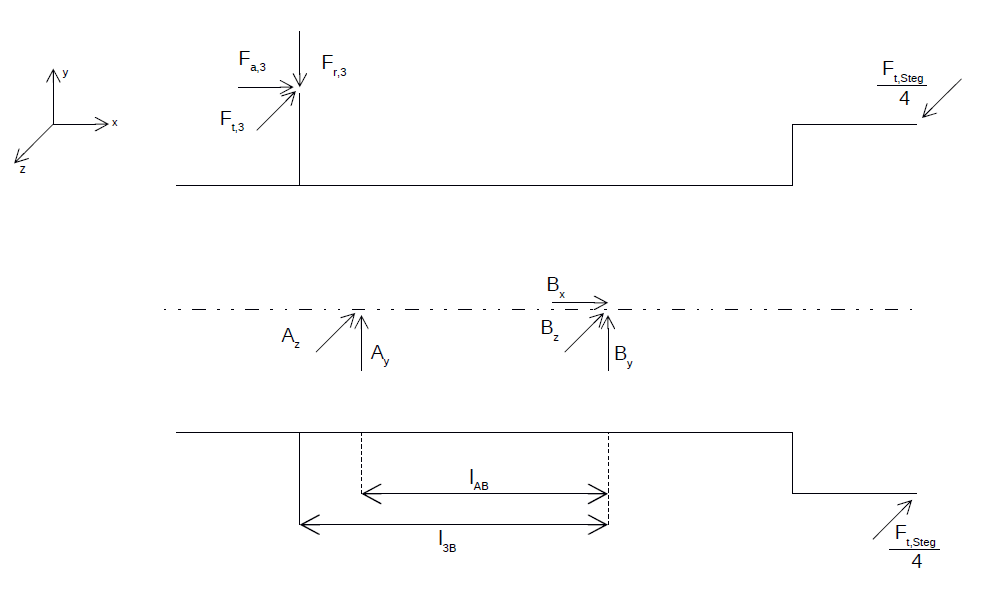
\includegraphics[width=1.04\textwidth,keepaspectratio]{figures/Hohlwelle.png}
\end{center}
\begin{itemize}
	\item Gegebene Werte: 
\begin{align*}
	&l_{AB} =171\text{ mm} \text{ , } l_{3B} = 175,8\text{ mm} \text{ , } d_{3} = 217,1\text{ mm}\\
	&F_{t,3} = 2633,53 \text{ N} \text{ , } F_{r,3}  = 1020,04\text{ N} \text{ , } F_{a,3} = 958,53 \text{ N}
\end{align*}
	\item Momentensummen:
\begin{align*}
	 \sum M\textsubscript{y}\textsuperscript{(B)} &\overset{!}{=} 0 = -A_z \x l_{AB} - F_{t,3} \x l_{3B} \\
	 	&\implies A_z = -F_{t,3} \x \frac{l_{3B}}{l_{AB}} = -2707,45 \text{ N} \\ \\
	 \sum M\textsubscript{z}\textsuperscript{(B)} &\overset{!}{=} 0 = -A_y \x l_{AB} + F_{r,3} \x l_{3B} - F_{a,3} \x \frac{d_3}{2}\\
	 	&\implies A_y = \frac{F_{r,3} \x l_{3B} - F_{a,3} \x \frac{d_3}{2}} {l_{AB}}= 440,2 \text{ N} 
\end{align*}
\end{itemize}
\section{Berechnung der Lagerreaktionen von Welle II}
\begin{center}
	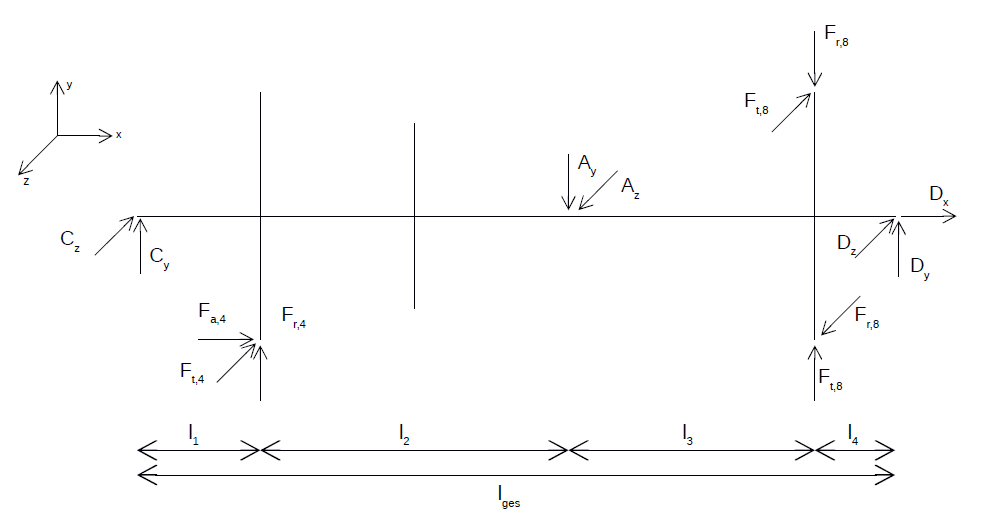
\includegraphics[width=1.04\textwidth,keepaspectratio]{figures/Uebersicht.png}
\end{center}
\begin{itemize}
	\item Gegebene Werte: 
	\begin{align*}
	&l_{1} =118,5\text{ mm} \text{ , } l_{2} = 226,5\text{ mm} \text{ , } l_{3} = 273 \text{ mm} \text{ , } l_{4} = 47\text{ mm} \text{ , } l_{ges} = 665\text{ mm} \\
	&d_4 = 89,4\text{ mm} \text{ , } d_8 = 112 \text{ mm} \\
	&F_{t,4} = 1598,88 \text{ N} \text{ , } F_{r,4}  = 619,29\text{ N} \text{ , } F_{a,4} = 581,94 \text{ N} \\
	&F_{t,8} = 319,1 \text{ N} \text{ , } F_{r,8}  = 116,13\text{ N}
\end{align*}
	\item Gleichgewichte:
\begin{align*}
    \sum F_x &\overset{!}{=} 0 = F_{a,4} + D_x \implies D_x = -F_{a,4} = -581,94 \text{ N} \\
    \sum F_y &\overset{!}{=} 0 = C_y + F_{r,4}-A_y +D_y - F_{r,8} + F_{r,8}\\ 
    \sum F_z &\overset{!}{=} 0 = A_z - C_z - D_z - F_{t,4} + F_{t,8} - F_{t,8}\\ \\
    \sum M\textsubscript{y}\textsuperscript{(D)} &\overset{!}{=} 0 = A_z \x (l_3+l_4)- F_{t,4} \x (l_2+l_3+l_4) - C_z \x l_{ges} +l_4 \x F_{t,8}- l_4 \x F_{t,8} \\ 
    &\implies C_z = \frac{(l_3+l_4) \x A_z - F_{t,4} \x (l_2+l_3+l_4)}{l_{ges}} = -2616,8 \text { N} \\ 
    & \implies D_z = A_z - C_z - F_{t,4}= -1689,53 \text{ N}\\ \\
    \sum M\textsubscript{z}\textsuperscript{(D)} &\overset{!}{=} 0 = (l_3+l_4) \x A_y + \frac{d_4}{2} \x F_{a,4} - (l_2+l_3+l_4) \x F_{r,4}- l_{ges} \x C_y  \\ 
    &\implies C_y = \frac{(l_3+l_4) \x A_y + \frac{d_4}{2} \x F_{a,4} - (l_2+l_3+l_4) \x F_{r,4}}{l\textsubscript{ges}} = -258 \text{ N}\\ 
    & \implies D_y =   A_y - C_y - F_{r,4} =  78,9\text{ N}\\ 
\end{align*}
\begin{align*}
    C_x &= \underline{0\text{ N}} & D_x= \underline{-581,94\text{ N}}\\
    C_y &= \underline{-258\text{ N}} & D_y= \underline{78,9\text{ N}}\\
    C_z &= \underline{-2616,8\text{ N}} & D_z= \underline{-1689,53\text{ N}}\\
\end{align*}
\end{itemize}
\newpage
\section{Berechnung der Schnittkraftverläufe}
\renewcommand{\labelenumi}{\roman{enumi})}
\begin{enumerate}
\item Bereich I: $0 \leq x_1 \leq l_1$
\begin{center}
	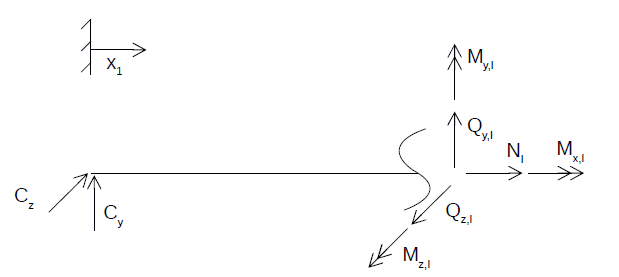
\includegraphics[width=1.04\textwidth,keepaspectratio]{figures/Bereich1.png}
\end{center}
    \begin{align*}
        \sum F_x &\overset{!}{=} 0 = N_{\mathrm{I}} \quad \implies \quad  N_{\mathrm{I}} = 0 \text{ N}\\ 
        \sum F_y &\overset{!}{=} 0 =  Q_{y,\mathrm{I}} + C_y \quad \implies \quad  Q_{y,\mathrm{I}} = -C_y = 258\text{ N}\\
        \sum F_z &\overset{!}{=} 0 =  Q_{z,\mathrm{I}} - C_z \quad \implies \quad  Q_{z,\mathrm{I}} = C_z = -2616,8\text{ N}\\
        \sum M_x \textsuperscript{(P)}&\overset{!}{=} 0 = M_{x,\mathrm{I}} \quad \implies \quad   M_{x,\mathrm{I}} = 0 \text{ Nm} \\ 
        \sum M_y \textsuperscript{(P)}&\overset{!}{=} 0 = M_{y,\mathrm{I}} - x_1 \x C_z \quad \implies \quad   M_{y,\mathrm{I}} =x_1 \x C_z =-2616,8 \text{ N} \x x_1\\ 
        \sum M_z \textsuperscript{(P)}&\overset{!}{=} 0 = M_{z,\mathrm{I}} -x_1 \x C_y  \quad \implies \quad   M_{z,\mathrm{I}} = x_1 \x C_y = -258 \text{ N} \x x_1 \\ 
    \end{align*}
\newpage
\item Bereich II: $0 \leq x_2 \leq l_2$
\begin{center}
	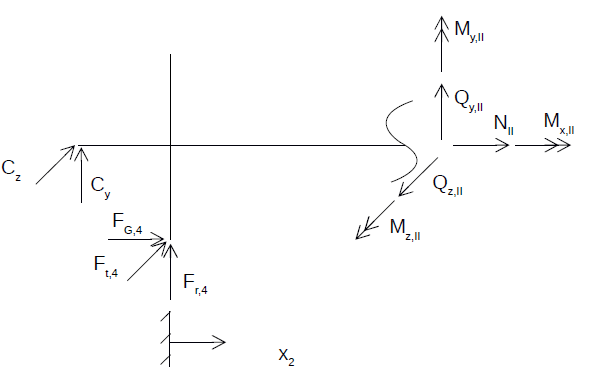
\includegraphics[width=0.93\textwidth,keepaspectratio]{figures/Bereich2.png}
\end{center}
\begin{align*}
        \sum F_x &\overset{!}{=} 0 = F_{a,4} + N_{\mathrm{II}} 
				\implies  N_{\mathrm{II}} = - F_{a,4}  =-581,94 \text{ N}\\ 
       \sum F_y &\overset{!}{=} 0 =C_y +F_{r,4} + Q_{y,\mathrm{II}} 
       		\implies  Q_{y,\mathrm{II}} = -C_y - F_{r,4} =-361,29 \text{ N}\\ 
       	\sum F_z &\overset{!}{=} 0 =-C_z -F_{t,4} + Q_{z,\mathrm{II}} 
       		\implies  Q_{z,\mathrm{II}} = C_z + F_{t,4} =-1017,92 \text{ N}\\ \\
        \sum M\textsubscript{x}\textsuperscript{(P)} &\overset{!}{=} 0 = M_{x,\mathrm{II}} + r_4 \x F_{t,4} \\
				&\implies M_{x,\mathrm{II}} = - \frac{d_4}{2} \x F_{t,4}  =  -71,5 \text{ Nm} \\ \\
		\sum M\textsubscript{y}\textsuperscript{(P)} &\overset{!}{=} 0 = M_{y,\mathrm{II}} - x_2 \x F_{t,4} - (l_1 + x_2) \x C_z \\
				&\implies M_{y,\mathrm{II}} = (l_1 + x_2) \x C_z +x_2 \x F_{t,4}  = -310,1\text{ Nm} -1017,92 \text{ N} \x x_2\\ \\
		\sum M\textsubscript{z}\textsuperscript{(P)} &\overset{!}{=} 0 = M_{z,\mathrm{II}} + \frac{d_4 }{2} \x F_{a,4} - x_2 \x F_{r,4} - (l_1 + x_2) \x )C_y \\ 
				&\implies M_{z,\mathrm{II}} = -\frac{d_4}{2} \x F_{a,4} + x_2 \x F_{r,4} + (l_1 + x_2) \x )C_y \\
				&= -56,59 \text{ Nm} + 361,29 \text{ N} \x x_2 \\
\end{align*}
\newpage
\item Bereich III: $0 \leq x_3 \leq l_3$
\begin{center}
	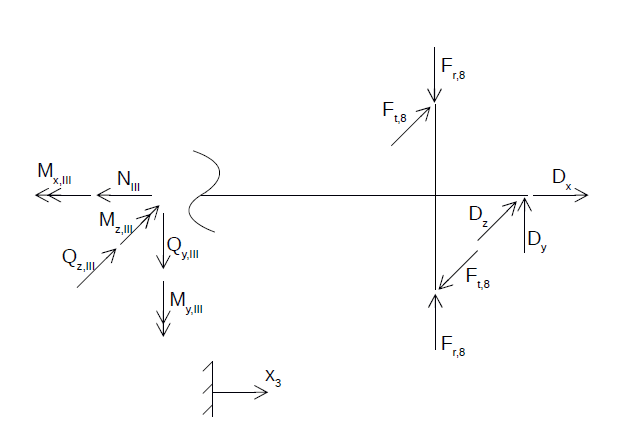
\includegraphics[width=0.93\textwidth,keepaspectratio]{figures/Bereich3.png}
\end{center}
	\begin{align*}
        \sum F_x &\overset{!}{=} 0 = D_x - N_{\mathrm{III}} 
				\implies  N_{\mathrm{III}} = D_x = -581,94 \text { N}\\ 
        \sum F_y &\overset{!}{=} 0 =D_y - Q_{y,\mathrm{III}} -F_{r,8} +F_{r,8}
				\implies Q_{y,\mathrm{III}} = D_y = 78,9 \text{ N}\\ 
		\sum F_z &\overset{!}{=} 0 = -D_z -Q{z,\mathrm{III}} +F_{t,8} - F_{t,8}
				\implies Q_{z,\mathrm{III}} = -D_z =1689,53 \text{ N} \\ \\
        \sum M\textsubscript{x}\textsuperscript{(P)} &\overset{!}{=} 0 =- M_{x,\mathrm{III}} - 4 \x \frac{d_8}{2}\x F_{t,8} \\
				&\implies M_{x,\mathrm{III}} = - 4 \x \frac{d_8}{2}\x F_{t,8} = -71,5 \text{ Nm} \\ \\
		\sum M\textsubscript{y}\textsuperscript{(P)} &\overset{!}{=} 0 =- M_{y,\mathrm{III}} + D_z \x (l_4+(l_3- x_3)) + F_{t,8} \x (l_3-x_3 )- F_{t,8} \x (l_3-x_3)\\
				&\implies M_{y,\mathrm{III}} = (l_4 + (l_3 - x_3)) \x D_z =-540,65 \text{ Nm} +1689,53 \text{ N} \x x_3\\ \\
		\sum M\textsubscript{z}\textsuperscript{(P)} &\overset{!}{=} 0 = - M_{z,\mathrm{III}} + D_y \x (l_4 + (l_3 - x_3)) + F_{r,8} \x (l_3 -x_3) - F_{r,8} \x (l_3 - x_3) \\
				&\implies  M_{z,\mathrm{III}} =  D_y \x (l_4 + (l_3 - x_3)) = 25,25 \text{ Nm} -78,9 \text{ N} \x x_3\\
	\end{align*}
\item Bereich IV: $0 \leq x_4 \leq l_4$
\begin{center}
	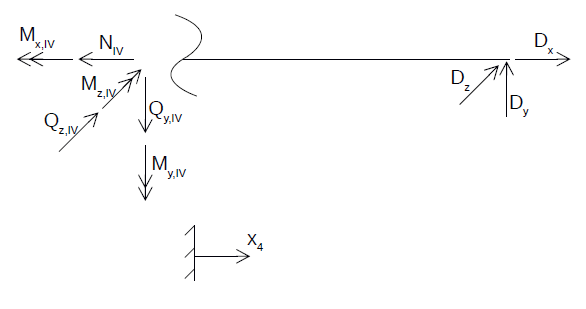
\includegraphics[width=1.04\textwidth,keepaspectratio]{figures/Bereich4.png}
\end{center}
\begin{align*}
	\sum F_x &\overset{!}{=} 0 = D_x - N_{\mathrm{IV}} 
		\implies  N_{\mathrm{IV}} = D_x = -581,94 \text { N}\\ 
	\sum F_y &\overset{!}{=} 0 =D_y - Q_{y,\mathrm{IV}}
		\implies Q_{y,\mathrm{IV}} = D_y = 78,9 \text{ N}\\ 
	\sum F_z &\overset{!}{=} 0 = -D_z -Q{z,\mathrm{IV}} 
		\implies Q_{z,\mathrm{IV}} = -D_z = 1689,53 \text{ N} \\ \\
	\sum M\textsubscript{x}\textsuperscript{(P)} &\overset{!}{=} 0 =- M_{x,\mathrm{IV}}  
		\implies M_{x,\mathrm{IV}} = 0 \text{ Nm} \\ \\
	\sum M\textsubscript{y}\textsuperscript{(P)} &\overset{!}{=} 0 =- M_{y,\mathrm{IV}} + D_z \x  (l_4 - x_4) \\
		&\implies M_{y,\mathrm{IV}} =  (l_4 - x_4) \x D_z =-79,4\text{ Nm} +1689,53 \text{ N} \x x_4\\ \\
	\sum M\textsubscript{z}\textsuperscript{(P)} &\overset{!}{=} 0 = - M_{z,\mathrm{IV}} + D_y \x  (l_4 - x_4)  \\
		&\implies  M_{z,\mathrm{IV}} =  D_y \x (l_4 - x_4) = 3,7\text{ Nm} -78,9 \text{ N} \x x_4
	\end{align*}
\end{enumerate}
\newpage
\textbf{Eckwerte:}\\ \\
Bereich i)
\begin{align*}
	N_{\mathrm{I}} (0) &= N_{\mathrm{I}} (l_1) = 0 \text{ N}\\
	Q_{y,\mathrm{I}} (0) &= Q_{y,\mathrm{I}} (l_1) = 258\text{ N}\\
	Q_{z,\mathrm{I}} (0) &= Q_{z,\mathrm{I}} (l_1) = -2616,8\text{ N}\\
	M_{x,\mathrm{I}} (0) &=  M_{x,\mathrm{I}} (l_1) = 0\text{ Nm}\\
	M_{y,\mathrm{I}} (0) &=  0\text{ Nm} & M_{y,\mathrm{I}} (l_1) &= -310,1\text{ Nm}\\
	M_{z,\mathrm{I}} (0) &= 0\text{ Nm} & M_{z,\mathrm{I}} (l_1) &= -30,57\text{ Nm}\\
\end{align*}
Bereich ii)
\begin{align*}
	N_{\mathrm{II}} (0) &= N_{\mathrm{II}} (l_2) = -581,94 \text{ N}\\
	Q_{y,\mathrm{II}} (0) &= Q_{y,\mathrm{II}} (l_2) =-361,29\text{ N}\\
	Q_{z,\mathrm{II}} (0) &= Q_{z,\mathrm{II}} (l_2) = -1017,92\text{ N}\\
	M_{x,\mathrm{II}} (0) &= M_{x,\mathrm{II}} (l_2) = -71,5\text{ Nm}\\
	M_{y,\mathrm{II}} (0) &=  -310,1 \text{ Nm} & M_{y,\mathrm{II}} (l_2) &= -540,65\text{ Nm}\\
	M_{z,\mathrm{II}} (0) &=  -56,59\text{ Nm} &M_{z,\mathrm{II}} (l_2) &= 25,25\text{ Nm}\\
\end{align*}
Bereich iii)
\begin{align*}
	N_{\mathrm{III}} (0) &= N_{\mathrm{III}} (l_3) = -581,94 \text{ N}\\
	Q_{y,\mathrm{III}} (0) &= Q_{y,\mathrm{III}} (l_3) =78,9\text{ N}\\
	Q_{z,\mathrm{III}} (0) &= Q_{z,\mathrm{III}} (l_3) = 1689,53\text{ N}\\
	M_{x,\mathrm{III}} (0) &= M_{x,\mathrm{III}} (l_3) = -71,5\text{ Nm}\\
	M_{y,\mathrm{III}} (0) &=  -540,65\text{ Nm} & M_{y,\mathrm{III}} (l_3) &= -79,4\text{ Nm}\\
	M_{z,\mathrm{III}} (0) &= 25,25\text{ Nm} &M_{z,\mathrm{III}} (l_3) &= 3,7\text{ Nm}\\
\end{align*}
Bereich iv)
\begin{align*}
	N_{\mathrm{IV}} (0) &= N_{\mathrm{IV}} (l_4) = -581,94 \text{ N}\\
	Q_{y,\mathrm{IV}} (0) &= Q_{y,\mathrm{IV}} (l_4) = 78,9\text{ N}\\
	Q_{z,\mathrm{IV}} (0) &= Q_{z,\mathrm{IV}} (l_4) = 1689,53\text{ N}\\
	M_{x,\mathrm{IV}} (0) &= M_{x,\mathrm{IV}} (l_4) = 0\text{ Nm}\\
	M_{y,\mathrm{IV}} (0) &=  -79,4\text{ Nm} & M_{y,\mathrm{IV}} (l_4) &= 0\text{ Nm}\\
	M_{z,\mathrm{IV}} (0) &= 3,7\text{ Nm} &M_{z,\mathrm{IV}} (l_4) &= 0\text{ Nm}\\
\end{align*}
\newpage
\section{Resultierende Momente}
\[
	|M_{b,res}(x)| = \sqrt{\left( M_{y}(x) \right)^2 + \left( M_{z}(x) \right)^2 }
\]
Bereich i)
\begin{align*}
	&|M_{b,res}(x=0)| = 0 \text{ Nm} \\
	&|M_{b,res}(x=l_1)| = 311,6 \text{ Nm} \\
\end{align*}
Bereich ii)
\begin{align*}
	&|M_{b,res}(x=l_1)| = 315,22 \text{ Nm} \\
	&|M_{b,res}(x=l_1+l_2)| = 541,24 \text{ Nm} \\
\end{align*}
Bereich iii)
\begin{align*}
	&|M_{b,res}(x=l_1+l_2)| = 541,24 \text{ Nm} \\
	&|M_{b,res}(x=l_1+l_2+l_3)| = 79,5 \text{ Nm} \\
\end{align*}
Bereich iv)
\begin{align*}
	&|M_{b,res}(x=l_1+l_2+l_3)| = 79,5 \text{ Nm} \\
	&|M_{b,res}(x=l_{ges})| = 0 \text{ Nm} \\
\end{align*}
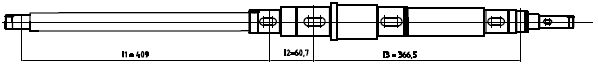
\includegraphics[width=\textwidth,keepaspectratio]{figures/Welle1klein.png}
	\chapter{Dauerfestigkeitsberechnung für Welle I}
In diesem Kapitel werden die beiden am meisten gefährdeten Querschnitte der Welle I auf Dauerfestigkeit und bleibende Verformung untersucht. Der Sicherheitsfaktor sollte dabei nach DIN 743 mindestens $S_{min} = 1,2$ betragen.
\section{Werkstoffkennwerte}
Als Werkstoff wurde der Vergütungsstahl 30CrNiMo8 gewählt. Die folgenden Festigkeitswerte stammen aus der Tabelle A.4 der DIN 743 - 3.
\begin{align*}
	&R_{p0,2} = 1050 \frac{\text{ N}}{\text{ mm}^2} = \sigma_S \\
	&R_{m} = 1250 \frac{\text{ N}}{\text{ mm}^2} = \sigma_B \\
	&\sigma_{zdW} = 500 \frac{\text{ N}}{\text{ mm}^2} \\
	&\sigma_{bW} = 625 \frac{\text{ N}}{\text{ mm}^2} \\
	&\tau_{tW} = 375 \frac{\text{ N}}{\text{ mm}^2} 
\end{align*}

\section{Freistichberechnung}
Die Sicherheit des Freistiches wird bei Umlaufbiegung und konstanter Torsions- und Zug-Druck-Beanspruchung berechnet.
\subsubsection{Abmessungen:}
\begin{align*}
	&D= 47 \text{ mm} & \frac{r}{t} = 0,21 \\
	&d= 39,4 \text{ mm} & \frac{r}{d} = 0,02 \\
	& r= 0,8 \text{ mm} & \frac{d}{D} = 0,838 \\
	& t= \frac{D-d}{2} = 3,8 \text{ mm} 
\end{align*}
\subsubsection{Wirkende Spannungen (nach DIN 743 - 1 Tabelle 1)}
\begin{align*}
	&\sigma_{zda} = \frac{F_{zda}}{A} = \frac{N}{\frac{\pi \x d^2}{4}} = \frac{581,94 \text{ N}}{1219,22 \text{ mm}^2} = 0,48 \frac{\text{ N}}{\text{ mm}^2} \\
	&\sigma_{ba} = \frac{M_{ba}}{A} = \frac{|M_{b,res}(x=345 \text{ mm}) |}{\frac{\pi \x d^3}{32}} = \frac{586480 \text{ Nmm}}{6004,66 \text{ mm}^3} = 97,67 \frac{\text{ N}}{\text{ mm}^2} \\
	&\tau_{ta} = \frac{M_{ta}}{A} = \frac{M_{\mathrm{II}}}{\frac{\pi \x d^3}{16}} = \frac{71500 \text{ Nmm}}{12009,32 \text{ mm}^3} = 5,95 \frac{\text{ N}}{\text{ mm}^2} 
\end{align*}
\subsubsection{Gesamteinflussfaktor}
Die folgenden Formeln stammen, soweit nichts anderes vermerkt, aus der DIN 743 - 2.
\begin{itemize}
\item Bezogenes Spannungsgefälle $G'$ \hfill (Tabelle 2)
	\begin{align*}
		\text{Hilfsgröße } \Phi &= \frac{1}{4 \x \sqrt{\frac{t}{r}} +2} = 0,09 \\
		G'_{ZD} &= \frac{2,3 \x (1+\Phi)}{r} = 3,13 \frac{1}{\text{ mm}} \\
		G'_{B}&= G'_{ZD}  =3,13 \frac{1}{\text{ mm}} \\
		G'_{T}&= \frac{1,15}{r} = 1,44\frac{1}{\text{ mm}} 
	\end{align*}
\item Technologischer Größeneinflussfaktor $K_1 (d_{eff})$ 
	\begin{align*}
		&\text{zur Vereinfachung wird angenommen } d_{eff} = D =47 \text{ mm und } d_B = 16 \text{ mm} \\ 
		&\text{Streckgrenze Vergütungsstahl: }K_{1,Re}(d_{eff}) = 1 - 0,34 \lg \left( \frac{d_{eff}}{d_B} \right) = 0,84  &(14) \\
		&\text{Zugfestigkeit Vergütungsstahl: } K_{1,Rm}(d_{eff}) = 1 - 26 \lg \left( \frac{d_{eff}}{d_B} \right) = 0,88  &(12) 
	\end{align*}
\item Formzahl $\alpha$
	\begin{align*}
		&\alpha_{\sigma ZD} = 1 + \frac{1}{\sqrt{0,62 \x \frac{r}{t} + 7 \x \frac{r}{d} (1+2 \x \frac{r}{d})^2}} = 2,88 & \text{(Bild 8)} \\
		&\alpha_{\sigma B} = 1 + \frac{1}{\sqrt{0,62 \x \frac{r}{t} + 11,6 \x \frac{r}{d} (1+2 \x \frac{r}{d})^2 + 0,2 \x \left( \frac{r}{t} \right) ^3 \x \frac{d}{D}}} = 2,62 & \text{(Bild 9)} \\
		&\alpha_{\tau} = 1 + \frac{1}{\sqrt{3,4 \x \frac{r}{t} + 38 \x \frac{r}{d} (1+2 \x \frac{r}{d})^2 + \left( \frac{r}{t} \right) ^2 \x \frac{d}{D}}} = 1,8  & \text{(Bild 10)} 
	\end{align*}
\item Stützziffer n \hfill (5)
	\begin{align*}
		n&= 1 + \sqrt{G' \x \text{ mm}} \x 10 ^{-\left( 0,33 + \frac{\sigma_S (d)}{712\frac{\text{ N}}{\text{ mm}^2}} \right)} \\
		\text{mit } \sigma_S (d) &= K_{1,Re} (d_{eff}) \x \sigma_S (d_B) \\
		&= 0,84 \x 1050 \frac{\text{ N}}{\text{ mm}^2} = 882 \frac{\text{ N}}{\text{ mm}^2} \\
		n_{ZD} &= n_B = 1 + \sqrt{3,13} \x 10 ^{-\left( 0,33 + \frac{882}{712} \right)} \\
		&=1,048 \\
		n_{\tau} &= 1 + \sqrt{1,44} \x 10 ^{-\left( 0,33 + \frac{882}{712} \right)} \\
		&= 1,032 
	\end{align*}
	Formel für $\sigma_S$ aus Skript KL III \ccite{bib:poll:kl3} S.168
\item Kerbwirkungszahl $\beta$ \hfill (4)
	\begin{align*}
		&\beta_{\sigma ZD} = \frac{\alpha_{\sigma ZD}}{n_{ZD}} = 2,748 \\
		&\beta_{\sigma B} = \frac{\alpha_{\sigma B}}{n_{B}} = 2,5 \\
		&\beta_{ \tau} = \frac{\alpha_{\sigma \tau}}{n_{\tau}} = 1,744 
	\end{align*}
\item Geometrischer Größeneinflussfaktor $K_2 (d)$ 
	\begin{align*}
		&\text{Zug/Druck: }K_{2ZD} (d) = 1 & (15) \\
		&\text{Biegung/Torsion: } K_{2B,\tau} (d) = 1 -0,2 \x  \frac{\lg (d / 7,5 \text{ mm})}{lg 20}  = 0,89 &(16) 
	\end{align*}
\item Einflussfaktor der Oberflächenrauheit $K_{F\sigma, \tau}$ (Skript KL III \ccite{bib:poll:kl3} S.171)
	\begin{align*}
		\text{Zug/Druck \& Biegung: } K_{F\sigma} &= 1 - 0,22 \x \lg \left( \frac{Rz}{\mu m}\right) \x ( \lg \left( \frac{\sigma_B (d)}{20}\frac{\text{ N}}{\text{ mm}^2}\right) -1 ) &(18) \\
		\text{mit } \sigma_B (d) &= K_{1,Re} (d_{eff}) \x \sigma_B (d_B) \\
		&= 0,84 \x 1250\frac{\text{ N}}{\text{ mm}^2} = 1050 \frac{\text{ N}}{\text{ mm}^2} \\
		\implies K_{F\sigma} &= 0,873 \text{ mit } R_z = 6,3 \mu m\\
		\text{Torsion: } K_{F\tau} &= 0,575 \x K_{F\sigma} +0,425 = 0,927 & (19) 
	\end{align*}
\item Einflussfaktor der Oberflächenverfestigung (aus dem Skript KL III \ccite{bib:poll:kl3} Seite 172)
	\[
		K_{V} = 1
	\]
\item Gesamteinflussfaktor $K_{\sigma}$ nach DIN 743 - 1
	\begin{align*}
		\text{Zug/Druck: } K_{\sigma ZD} &= \left( \frac{\beta_{\sigma ZD}}{K_{2ZD} (d)} + \frac{1}{K_{F\sigma}} -1\right) \x \frac{1}{K_V} & (8) \\
		&= \left( \frac{2,748}{1} + \frac{1}{0,873} -1\right) \x \frac{1}{1} \\
		&= 2,893 \\
		\text{Biegung: } K_{\sigma B} &= \left( \frac{\beta_{\sigma B}}{K_{2B}(d)} + \frac{1}{K_{F\sigma}} -1\right) \x \frac{1}{K_V} & (8) \\
		&= \left( \frac{2,5}{0,89} + \frac{1}{0,873} -1\right) \x \frac{1}{1} \\
		&= 2,954 \\
		\text{Torsion: } K_{\tau} &= \left( \frac{\beta_{\tau}}{K_{2\tau}(d)} + \frac{1}{K_{F\tau}} -1\right) \x \frac{1}{K_V} & (9) \\
		&= \left( \frac{1,744}{0,89} + \frac{1}{0,927} -1\right) \x \frac{1}{1} \\
		&= 1,15 
	\end{align*}
\end{itemize}
\subsubsection{Vorhandene Sicherheitszahl für Dauerfestigkeitsnachweis nach Belastungsfall 1 }
verwendete Formeln aus der DIN 743 - 1
\begin{itemize}
\item Vergleichsmittelspannung 
	\begin{align*}
	\sigma_{mv}&= \sqrt{(\sigma_{zdm} +\sigma_{bm} )^2+ 3 \x \tau_{tm}^2 } & (23) \\
	&\sigma_{bm}= 0 \text{ (da Umlaufbiegung vorliegt)} \\
	&\sigma_{zdm} = \sigma_{zda} = 0,48\frac{\text{ N}}{\text{ mm}^2} \\
	&\tau_{tm} = \tau_{ta} = 5,95 \frac{\text{ N}}{\text{ mm}^2} \\
	\implies \sigma_{mv}&= \sqrt{(0,48 \frac{\text{ N}}{\text{ mm}^2} +0 )^2+ 3 \x (5,95 \frac{\text{ N}}{\text{ mm}^2})^2 }  \\
	&= 10,32 \frac{\text{ N}}{\text{ mm}^2} \\
	\tau_{mv} &= \frac{\sigma_{mv}}{\sqrt{3}} = 5,96 \frac{\text{ N}}{\text{ mm}^2} & (24)
	\end{align*}
\item Bauteilwecheselfestigkeit $\sigma_{WK}$ 
	\begin{align*}
	\sigma_{zdWK}&= \frac{\sigma_{zdW} \x K_{1,Rm} (d_{eff})}{K_{\sigma ZD}}  & (5)\\
	&=  \frac{500 \frac{\text{ N}}{\text{ mm}^2}\x 0,88}{2,893} = 152,09 \frac{\text{ N}}{\text{ mm}^2}\\
	\sigma_{bWK}&= \frac{\sigma_{bW} \x K_{1,Rm} (d_{eff})}{K_{\sigma B}}  & (6 )\\
	&=  \frac{625 \frac{\text{ N}}{\text{ mm}^2}\x 0,88}{2,954} = 186,19 \frac{\text{ N}}{\text{ mm}^2}\\
	\tau_{tWK}&= \frac{\tau_{tW} \x K_{1,Rm} (d_{eff})}{K_{\tau}} &(7) \\
	&=  \frac{375 \frac{\text{ N}}{\text{ mm}^2}\x 0,88}{1,15} = 286,96 \frac{\text{ N}}{\text{ mm}^2}
	\end{align*}
\item Einflussfaktor der Mittelspannungsempfindlichkeit $\Psi_{K}$ 
	\begin{align*}
	\Psi_{zd \sigma K}&= \frac{\sigma_{zdWK}}{2 \x  K_{1,Rm} (d_{eff}) \x \sigma_B (d_B) -\sigma_{zdWK}}  &(20)\\
	&=  \frac{152,09 \frac{\text{ N}}{\text{ mm}^2}}{2 \x 0,88 \x 1250\frac{\text{ N}}{\text{ mm}^2} - 152,09 \frac{\text{ N}}{\text{ mm}^2}} = 0,074 \\
	\Psi_{b \sigma K}&= \frac{\sigma_{bWK}}{2 \x  K_{1,Rm} (d_{eff}) \x \sigma_B (d_B) -\sigma_{bWK}} &(21) \\
	&=  \frac{186,19 \frac{\text{ N}}{\text{ mm}^2}}{2 \x 0,88 \x 1250\frac{\text{ N}}{\text{ mm}^2} - 186,19 \frac{\text{ N}}{\text{ mm}^2}} = 0,092 \\
	\Psi_{\tau K}&= \frac{\tau_{tWK}}{2 \x  K_{1,Rm} (d_{eff}) \x \sigma_B (d_B) -\tau_{tWK}} &(22) \\
	&=  \frac{286,96 \frac{\text{ N}}{\text{ mm}^2}}{2 \x 0,88 \x 1250\frac{\text{ N}}{\text{ mm}^2} - 286,96 \frac{\text{ N}}{\text{ mm}^2}} = 0,15 
	\end{align*}
\item Spannungsamplitude der Bauteildauerfestigkeit
	\begin{align*}
	\sigma_{zdADK} &= \sigma_{zdWK} - \Psi_{zd \sigma K} \x \sigma_{mv} &(10) \\
	&= 152,09\frac{\text{ N}}{\text{ mm}^2} - 0,074 \x 10,32 \frac{\text{ N}}{\text{ mm}^2} = 151,33 \frac{\text{ N}}{\text{ mm}^2} \\
	\sigma_{bADK} &= \sigma_{bWK} - \Psi_{b \sigma K} \x \sigma_{mv} &(11) \\
	&= 186,19\frac{\text{ N}}{\text{ mm}^2} - 0,092 \x 10,32 \frac{\text{ N}}{\text{ mm}^2} = 185,24 \frac{\text{ N}}{\text{ mm}^2} \\
	\tau_{tADK} &= \tau_{tWK} - \Psi_{ \tau K} \x \tau_{mv} &(12) \\
	&= 286,96\frac{\text{ N}}{\text{ mm}^2} - 0,15 \x 5,96 \frac{\text{ N}}{\text{ mm}^2} = 286,07 \frac{\text{ N}}{\text{ mm}^2} 
	\end{align*}
\item vorhandene Sicherheitszahl S 
	\begin{align*}
		&S= \frac{1}{\sqrt{\left( \frac{\sigma_{zda}}{\sigma_{zdADK}} +\frac{\sigma_{ba}}{\sigma_{bADK}} \right)^2 +\left( \frac{\tau_{ta}}{\tau_{tADK}} \right)^2 }} &(2) \\
		&S=  1,88 
	\end{align*}
\end{itemize}
\subsubsection{Vorhandene Sicherheitszahl S für Nachweis gegen Überschreiten der Fließgrenze}
verwendete Formeln aus der DIN 743 - 1
\begin{itemize}
\item Statische Stützwirkung $K_{2F}$ nach Tabelle 3
	\begin{align*}
	&K_{2F \sigma zd} = 1 \\
	&K_{2F \sigma b} = 1,2 \\
	&K_{2F \tau} = 1,2 
	\end{align*}
\item Erhöhungsfaktor der Fließgrenze $\gamma_{F}$ nach Tabelle 2
	\begin{align*}
	&\gamma_{F\sigma} = 1,1 \text{ (Für } \beta_{\sigma} = 2,0 \text{ bis } 3,0 \text{)} \\
	&\gamma_{F\tau} = 1 
	\end{align*}
\item Bauteilfließgrenze
	\begin{align*}
	\sigma_{zd,bFK} &= K_{1,Re} (d_{eff}) \x K_{2F \sigma} \x \gamma_{F\sigma} \x \sigma_S (d_B) & (31) \\
	\sigma_{zdFK}&= 0,84 \x 1 \x 1,1 \x 1050 \frac{\text{ N}}{\text{ mm}^2} \\
	&= 970,2 \frac{\text{ N}}{\text{ mm}^2}\\
	\sigma_{bFK}&= 0,84 \x 1,2 \x 1,1 \x 1050 \frac{\text{ N}}{\text{ mm}^2} \\
	&= 1164,24\frac{\text{ N}}{\text{ mm}^2}\\
	\tau_{tFK} &= K_{1,Re} (d_{eff}) \x K_{2F \tau} \x \gamma_{F\tau} \x \sigma_S (d_B) / \sqrt{3} &(32) \\
	&= 0,84 \x 1,2 \x 1 \x 1050 \frac{\text{ N}}{\text{ mm}^2} / \sqrt{3}\\
	&= 1058,4 \frac{\text{ N}}{\text{ mm}^2}
	\end{align*}
\newpage
\item Vorhandene Sicherheitszahl S \\
	Für diesen Fall wird mit den wirkenden Spannungsamplituden als maximale Spannungen gerechnet, da keine stoßartige Belastung angenommen wird. 
	\begin{align*}
	&S = \frac{1}{\sqrt{\left( \frac{\sigma_{zdmax}}{\sigma_{zdFK}}+\frac{\sigma_{bmax}}{\sigma_{bFK}} \right)^2 +\left( \frac{\tau_{tmax}}{\tau_{tFK}} \right)^2 }} & (25)\\
	&= 11,82
	\end{align*}
\end{itemize}
Die Schwachstelle 1, also der Freistich, ist gegen Dauerbruch und plastische Verformung ausreichend ausgelegt.


\section{Berechnung der Sicherungsringnut}
Die Sicherheit der Sicherungsringnut wird bei Umlaufbiegung und konstanter Torsions- und Zug-Druck-Beanspruchung berechnet.
\subsubsection{Abmessungen:}
\begin{align*}
&D= 40 \text{ mm}  \\
&d= 37,5 \text{ mm}  \\
& m= 1,85 \text{ mm} \\
& r= 0,175 \text{ mm}\\
& t=\frac{D-d}{2} =1,25 \text{ mm} 
\end{align*}
\subsubsection{Wirkende Spannungen (nach DIN 743 - 1 Tabelle 1)}
\begin{align*}
&\sigma_{zda} = \frac{F_{zda}}{A} = \frac{N}{\frac{\pi \x d^2}{4}} = \frac{581,94 \text{ N}}{1104,47 \text{ mm}^2} = 0,53 \frac{\text{ N}}{\text{ mm}^2} \\
&\sigma_{ba} = \frac{M_{ba}}{A} = \frac{|M_{b,res}(x=345 \text{ mm}) |}{\frac{\pi \x d^3}{32}} = \frac{586480 \text{ Nmm}}{5177,19 \text{ mm}^3} = 113,28 \frac{\text{ N}}{\text{ mm}^2} \\
&\tau_{ta} = \frac{M_{ta}}{A} = \frac{M_{\mathrm{II}}}{\frac{\pi \x d^3}{16}} = \frac{71500 \text{ Nmm}}{10354,37 \text{ mm}^3} = 6,9 \frac{\text{ N}}{\text{ mm}^2} 
\end{align*}
\subsubsection{Gesamteinflussfaktor}
Die folgenden Formeln stammen, soweit nichts anderes vermerkt, aus der DIN 743 - 2. Als Bezugsdurchmesser dient $d_{BK} = 30$ mm.
\begin{itemize}
\item Bezogenes Spannungsgefälle $G'$ \hfill (Tabelle 2)
	\begin{align*}
	\text{Hilfsgröße } \Phi &= \frac{1}{4 \x \sqrt{\frac{t}{r}} +2} = 0,09 \\
	G'_{ZD} &= \frac{2,3 \x (1+\Phi)}{r} = 3,13 \frac{1}{\text{ mm}} \\
	G'_{B}&= G'_{ZD}  =3,13 \frac{1}{\text{ mm}} \\
	G'_{T}&= \frac{1,15}{r} = 1,44\frac{1}{\text{ mm}} 
	\end{align*}
\item Technologischer Größeneinflussfaktor $K_1 (d_{eff})$ 
	\begin{align*}
	&\text{zur Vereinfachung wird angenommen } d_{eff} = D =40 \text{ mm und } d_B = 16 \text{ mm} \\ 
	&\text{Streckgrenze Vergütungsstahl: }K_{1,Re}(d_{eff}) = 1 - 0,34 \lg \left( \frac{d_{eff}}{d_B} \right) = 0,86  &(14) \\
	&\text{Zugfestigkeit Vergütungsstahl: } K_{1,Rm}(d_{eff}) = 1 - 26 \lg \left( \frac{d_{eff}}{d_B} \right) = 0,897  &(12) 
	\end{align*}
\item Strukturradius $ \rho ^*$ nach Kapitel 4.2.4
	\begin{align*}
	\sigma_S (d) &= \sigma_S (d_B) \x K_{1,Re}(deff) = 1050 \frac{\text{ N}}{\text{ mm}^2} \x 0,86 = 903 \frac{\text{ N}}{\text{ mm}^2} &(Bild 3)\\ 
	\rho ^* &=10 ^{-\left(0,514+0,00152\x \sigma_S (d) / \left(\frac{\text{ N}}{\text{ mm}^2} \right) \right)} \x \text{ mm}= 0,013 \text{ mm}
	\end{align*}
\item korrigierter Rundungsradius $ r_f$ nach Kapitel 4.2.4
	\begin{align*}
	\text{Zug/Druck, Biegung: } r_{f,ZD} =& r_{f,B} = r + 2,9 \x \rho ^* = 0,175 \text{ mm} + 2,9 \x 0,013 \text{ mm} = 0,213 \text{ mm}\\ 
	\text{Torsion: } r_{f,\tau} =& r +  \rho ^* = 0,175 \text{ mm} + 0,013 \text{ mm} = 0,188\text{ mm}
	\end{align*}
\item Hilfsgröße $ \beta^* (d_{BK})$ nach Kapitel 4.2.4
	\begin{align*}
	\text{Zug/Druck: }\beta _{\sigma,ZD} ^* (d_{BK}) =& 0,9 \x (1,27 + 1,17 \x \sqrt{t/r_{f,ZD}})  = 3,694 \\ 
	\text{Biegung: }\beta _{\sigma,B} ^* (d_{BK}) =& 0,9 \x (1,14 + 1,08 \x \sqrt{t/r_{f,B}})  = 3,381 \\ 
	\text{Torsion: }\beta _{\tau} ^* (d_{BK}) =& (1,48 + 0,45 \x \sqrt{t/r_{f,\tau}})  = 2,64
	\end{align*}
\item Kerbwirkungszahl $\beta (d_{BK}) $ nach Kapitel 4.2.4
	\begin{align*}
	\text{Für } &m/t \ge 1,4 \text{ gilt: } \beta (d_{BK}) = \beta^* (d_{BK}) \\
	\implies &\beta_{\sigma,ZD} (d_{BK}) = 3,694 \\
	&\beta_{\sigma,B}(d_{BK}) = 3,381 \\
	&\beta_{ \tau} (d_{BK})= 2,64 
	\end{align*}
\item Geometrischer Größeneinflussfaktor $K_3 (d) $ und $K_3 (d_{BK}) $ \hfill (17)
	\begin{align*}
	& K_3 (d) = 1-0,2 \x lg(\beta (d_{BK})) \x \frac{lg(d/7,5 \text{ mm})}{lg(20)}\\
	&K_{3,ZD} (d) = 1-0,2 \x lg(3,694) \x \frac{lg(37,5/7,5 \text{ mm})}{lg(20)} =0,939\\
	&K_{3,B} (d) = 1-0,2 \x lg(3,381) \x \frac{lg(37,5/7,5 \text{ mm})}{lg(20)} =0,943\\
	&K_{3,\tau} (d) = 1-0,2 \x lg(2,64) \x \frac{lg(37,5/7,5 \text{ mm})}{lg(20)} =0,955\\ \\
	&K_{3,ZD} (d_{BK}) = 1-0,2 \x lg(3,694) \x \frac{lg(30/7,5 \text{ mm})}{lg(20)} =0,947\\
	&K_{3,B} (d_{BK}) = 1-0,2 \x lg(3,381) \x \frac{lg(30/7,5 \text{ mm})}{lg(20)} =0,951\\
	&K_{3,\tau} (d_{BK}) = 1-0,2 \x lg(2,64) \x \frac{lg(30/7,5 \text{ mm})}{lg(20)} =0,961
	\end{align*}
\item Kerbwirkungszahl $\beta (d) $ \hfill (3)
	\begin{align*}
	 &\beta (d) = \beta (d_{BK}) \x \frac{K_3 (d_{BK})}{K_3 (d)} \\
	 &\beta_{\sigma,ZD} (d) =  3,694 \x \frac{0,947}{0,939} = 3,725\\
	&\beta_{\sigma,B}(d) = 3,381 \x \frac{0,951}{0,943} =3,41\\
	&\beta_{ \tau} (d)= 2,64 \x \frac{0,961}{0,955}  =2,657
	\end{align*}
\item Geometrischer Größeneinflussfaktor $K_2 (d)$ 
	\begin{align*}
	&\text{Zug/Druck: }K_{2ZD} (d) = 1 & (15) \\
	&\text{Biegung/Torsion: } K_{2B,\tau} (d) = 1 -0,2 \x  \frac{\lg (d / 7,5 \text{ mm})}{lg 20}  = 0,893 &(16) 
	\end{align*}
\item Einflussfaktor der Oberflächenverfestigung (aus dem Skript KL III \ccite{bib:poll:kl3} Seite 172)
	\[
	K_{V} = 1
	\]
\item Einflussfaktor der Oberflächenrauheit $K_{F\sigma, \tau} (Rz)$
	\begin{align*}
	\text{Zug/Druck \& Biegung: } K_{F\sigma} (Rz)&= 1 - 0,22 \x \lg \left( \frac{Rz}{\mu m}\right) \x ( \lg \left( \frac{\sigma_B (d)}{20\frac{\text{ N}}{\text{ mm}^2}}\right) -1 ) &(18) \\
	\text{mit } \sigma_B (d) &= K_{1,Re} (d_{eff}) \x \sigma_B (d_B) \\
	&= 0,86 \x 1250\frac{\text{ N}}{\text{ mm}^2} = 1075 \frac{\text{ N}}{\text{ mm}^2} \\
	\implies K_{F\sigma} (Rz) & = 1 - 0,22 \x \lg \left( \frac{6,3 \mu m}{\mu m}\right) \x ( \lg \left( \frac{1075\frac{\text{ N}}{\text{ mm}^2} }{20\frac{\text{ N}}{\text{ mm}^2}}\right) -1 ) \\
	 &= 0,872 \\
	\text{Torsion: } K_{F\tau} (Rz)&= 0,575 \x K_{F\sigma} (Rz) +0,425 = 0,926 & (19) 
	\end{align*}
\item Einflussfaktor der Oberflächenrauheit $K_{F\sigma, \tau} (Rz_B)$
	\begin{align*}
	\text{Gültig für die Probe mit der } &\text{mittleren Rauheit der Kerbe } Rz_B= 20 \mu m\\
	\text{Zug/Druck \& Biegung: } K_{F\sigma} (Rz_B)&= 1 - 0,22 \x \lg \left( \frac{Rz_B}{\mu m}\right) \x ( \lg \left( \frac{\sigma_B (d)}{20}\frac{\text{ N}}{\text{ mm}^2}\right) -1 ) &(18) \\
	\implies K_{F\sigma} (Rz_B) & = 1 - 0,22 \x \lg \left( \frac{20 \mu m}{\mu m}\right) \x ( \lg \left( \frac{1075\frac{\text{ N}}{\text{ mm}^2} }{20\frac{\text{ N}}{\text{ mm}^2}}\right) -1 )\\
	&= 0,79 \\
	\text{Torsion: } K_{F\tau} (Rz_B)&= 0,575 \x K_{F\sigma} (Rz_B) +0,425 = 0,879 & (19) 
	\end{align*}
\item Einflussfaktor der Oberflächenrauheit $K_{F\sigma, \tau} $
	\begin{align*}
	\text{Zug/Druck \& Biegung: } K_{F\sigma} =&\frac{K_{F\sigma} (Rz)}{K_{F\sigma} (Rz_B)} = 1,104 &(20) \\
	\text{Torsion: } K_{F\tau} = &\frac{K_{F\tau} (Rz)}{K_{F\tau} (Rz_B)} = 1,053 &(20)
	\end{align*}
\item Gesamteinflussfaktor $K_{\sigma}$ nach DIN 743 - 1
	\begin{align*}
	\text{Zug/Druck: } K_{\sigma ZD} &= \left( \frac{\beta_{\sigma ZD}}{K_{2ZD} (d)} + \frac{1}{K_{F\sigma}} -1\right) \x \frac{1}{K_V} & (8) \\
	&= \left( \frac{3,725}{1} + \frac{1}{1,104} -1\right) \x \frac{1}{1} \\
	&= 3,631 \\
	\text{Biegung: } K_{\sigma B} &= \left( \frac{\beta_{\sigma B}}{K_{2B}(d)} + \frac{1}{K_{F\sigma}} -1\right) \x \frac{1}{K_V} & (8) \\
	&= \left( \frac{3,41}{0,893} + \frac{1}{1,104} -1\right) \x \frac{1}{1} \\
	&= 3,724 \\
	\text{Torsion: } K_{\tau} &= \left( \frac{\beta_{\tau}}{K_{2\tau}(d)} + \frac{1}{K_{F\tau}} -1\right) \x \frac{1}{K_V} & (9) \\
	&= \left( \frac{2,657}{0,893} + \frac{1}{1,053} -1\right) \x \frac{1}{1} \\
	&= 2,925 
	\end{align*}
\end{itemize}
\subsubsection{Vorhandene Sicherheitszahl für Dauerfestigkeitsnachweis nach Belastungsfall 1 }
verwendete Formeln aus der DIN 743 - 1
\begin{itemize}
	\item Vergleichsmittelspannung 
	\begin{align*}
	\sigma_{mv}&= \sqrt{(\sigma_{zdm} +\sigma_{bm} )^2+ 3 \x \tau_{tm}^2 } & (23) \\
	&\sigma_{bm}= 0 \text{ (da Umlaufbiegung vorliegt)} \\
	&\sigma_{zdm} = \sigma_{zda} = 0,53\frac{\text{ N}}{\text{ mm}^2} \\
	&\tau_{tm} = \tau_{ta} = 6,9 \frac{\text{ N}}{\text{ mm}^2} \\
	\implies \sigma_{mv}&= \sqrt{(4,22 \frac{\text{ N}}{\text{ mm}^2} +0 )^2+ 3 \x (6,9 \frac{\text{ N}}{\text{ mm}^2})^2 }  \\
	&= 11,96 \frac{\text{ N}}{\text{ mm}^2} \\
	\tau_{mv} &= \frac{\sigma_{mv}}{\sqrt{3}} = 6,9 \frac{\text{ N}}{\text{ mm}^2} & (24)
	\end{align*}
	\item Bauteilwecheselfestigkeit $\sigma_{WK}$ 
	\begin{align*}
	\sigma_{zdWK}&= \frac{\sigma_{zdW} \x K_{1,Rm} (d_{eff})}{K_{\sigma ZD}}  & (5)\\
	&=  \frac{500 \frac{\text{ N}}{\text{ mm}^2}\x 0,897}{3,631} = 123,52 \frac{\text{ N}}{\text{ mm}^2}\\
	\sigma_{bWK}&= \frac{\sigma_{bW} \x K_{1,Rm} (d_{eff})}{K_{\sigma B}}  & (6 )\\
	&=  \frac{625 \frac{\text{ N}}{\text{ mm}^2}\x 0,897}{3,724} = 150,54 \frac{\text{ N}}{\text{ mm}^2}\\
	\tau_{tWK}&= \frac{\tau_{tW} \x K_{1,Rm} (d_{eff})}{K_{\tau}} &(7) \\
	&=  \frac{375 \frac{\text{ N}}{\text{ mm}^2}\x 0,897}{2,925} = 115 \frac{\text{ N}}{\text{ mm}^2}
	\end{align*}
	\item Einflussfaktor der Mittelspannungsempfindlichkeit $\Psi_{K}$ 
	\begin{align*}
	\Psi_{zd \sigma K}&= \frac{\sigma_{zdWK}}{2 \x  K_{1,Rm} (d_{eff}) \x \sigma_B (d_B) -\sigma_{zdWK}}  &(20)\\
	&=  \frac{123,52 \frac{\text{ N}}{\text{ mm}^2}}{2 \x 0,897 \x 1250\frac{\text{ N}}{\text{ mm}^2} - 123,52 \frac{\text{ N}}{\text{ mm}^2}} = 0,058 \\
	\Psi_{b \sigma K}&= \frac{\sigma_{bWK}}{2 \x  K_{1,Rm} (d_{eff}) \x \sigma_B (d_B) -\sigma_{bWK}} &(21) \\
	&=  \frac{150,54 \frac{\text{ N}}{\text{ mm}^2}}{2 \x 0,897 \x 1250\frac{\text{ N}}{\text{ mm}^2} - 150,54 \frac{\text{ N}}{\text{ mm}^2}} = 0,072 \\
	\Psi_{\tau K}&= \frac{\tau_{tWK}}{2 \x  K_{1,Rm} (d_{eff}) \x \sigma_B (d_B) -\tau_{tWK}} &(22) \\
	&=  \frac{115 \frac{\text{ N}}{\text{ mm}^2}}{2 \x 0,897 \x 1250\frac{\text{ N}}{\text{ mm}^2} - 115 \frac{\text{ N}}{\text{ mm}^2}} = 0,054 
	\end{align*}
	\item Spannungsamplitude der Bauteildauerfestigkeit
	\begin{align*}
	\sigma_{zdADK} &= \sigma_{zdWK} - \Psi_{zd \sigma K} \x \sigma_{mv} &(10) \\
	&= 123,52\frac{\text{ N}}{\text{ mm}^2} - 0,058 \x 11,96 \frac{\text{ N}}{\text{ mm}^2} = 122,83 \frac{\text{ N}}{\text{ mm}^2} \\
	\sigma_{bADK} &= \sigma_{bWK} - \Psi_{b \sigma K} \x \sigma_{mv} &(11) \\
	&= 150,54\frac{\text{ N}}{\text{ mm}^2} - 0,072 \x 11,96 \frac{\text{ N}}{\text{ mm}^2} = 149,68\frac{\text{ N}}{\text{ mm}^2} \\
	\tau_{tADK} &= \tau_{tWK} - \Psi_{ \tau K} \x \tau_{mv} &(12) \\
	&= 115\frac{\text{ N}}{\text{ mm}^2} - 0,054 \x6,9 \frac{\text{ N}}{\text{ mm}^2} = 114,63 \frac{\text{ N}}{\text{ mm}^2} 
	\end{align*}
	\item vorhandene Sicherheitszahl S 
	\begin{align*}
	&S= \frac{1}{\sqrt{\left( \frac{\sigma_{zda}}{\sigma_{zdADK}} +\frac{\sigma_{ba}}{\sigma_{bADK}} \right)^2 +\left( \frac{\tau_{ta}}{\tau_{tADK}} \right)^2 }} &(2) \\
	&S=  1,3 
	\end{align*}
\end{itemize}
\subsubsection{Vorhandene Sicherheitszahl S für Nachweis gegen Überschreiten der Fließgrenze}
verwendete Formeln aus der DIN 743 - 1
\begin{itemize}
\item Statische Stützwirkung $K_{2F}$ nach Tabelle 3
	\begin{align*}
	&K_{2F \sigma zd} = 1 \\
	&K_{2F \sigma b} = 1,2 \\
	&K_{2F \tau} = 1,2 
	\end{align*}
\item Erhöhungsfaktor der Fließgrenze $\gamma_{F}$ nach Tabelle 2
	\begin{align*}
	&\gamma_{F\sigma} = 1,15 \text{ (Für } \beta_{\sigma} > 3,0 \text{)} \\
	&\gamma_{F\tau} = 1 
	\end{align*}
\item Bauteilfließgrenze
	\begin{align*}
	\sigma_{zd,bFK} &= K_{1,Re} (d_{eff}) \x K_{2F \sigma} \x \gamma_{F\sigma} \x \sigma_S (d_B) & (31) \\
	\sigma_{zdFK}&= 0,86 \x 1 \x 1,15 \x 1050 \frac{\text{ N}}{\text{ mm}^2} \\
	&= 1038,45 \frac{\text{ N}}{\text{ mm}^2}\\
	\sigma_{bFK}&= 0,86 \x 1,2 \x 1,15 \x 1050 \frac{\text{ N}}{\text{ mm}^2} \\
	&= 1246,14\frac{\text{ N}}{\text{ mm}^2}\\
	\tau_{tFK} &= K_{1,Re} (d_{eff}) \x K_{2F \tau} \x \gamma_{F\tau} \x \sigma_S (d_B) / \sqrt{3} &(32) \\
	&= 0,86 \x 1,2 \x 1 \x 1050 \frac{\text{ N}}{\text{ mm}^2} / \sqrt{3}\\
	&= 625,62 \frac{\text{ N}}{\text{ mm}^2}
	\end{align*}
	\newpage
\item Vorhandene Sicherheitszahl S \\
	Für diesen Fall wird mit den wirkenden Spannungsamplituden als maximale Spannungen gerechnet, da keine stoßartige Belastung angenommen wird. 
	\begin{align*}
	&S = \frac{1}{\sqrt{\left( \frac{\sigma_{zdmax}}{\sigma_{zdFK}}+\frac{\sigma_{bmax}}{\sigma_{bFK}} \right)^2 +\left( \frac{\tau_{tmax}}{\tau_{tFK}} \right)^2 }} & (25)\\
	&= 10,86 
	\end{align*}
\end{itemize}
Die Schwachstelle 2, also die Sicherungsringnut, ist ebenfalls gegen Dauerbruch und plastische Verformung ausreichend ausgelegt, da er die geforderte Sicherheit von 1,2 erfüllt.
	\newpage
\chapter{Lagerlebensdauerberechnung}
\section{Lagerkräfte im Gang 1}
\subsubsection{Berechnung der Zahnradkräfte}
Die Berechnung der Kräfte und die verwendeten Formeln entsprechen dem Kapitel 3.2. Im 1. Gang sind Z1/Z2 und Z6/Z7 im Eingriff.
\begin{itemize}
\item Gegebene Werte: 
	\begin{align*}
	&n_{\mathrm{II},1} = 400\frac{1}{\text{min}} \\
	&T_{\mathrm{II},1,S} = 18,4\text{ Nm} \\
	&T_{\mathrm{III},1,S} = 73,63\text{ Nm} \\	
	&d_2 = 217,1\text{ mm} \text{ , } d_6 = 149 \text{ mm , } d_8 = 112 \text{ mm}
	\end{align*}
\item Z2, Gang 1:
	\begin{align*} 
	&F_{t,2,1} = \frac{2\x T_{\mathrm{II},1,S}}{d_2} = \frac{2 \x 18,4 \text{ Nm}}{0,2171 \text{ m}} = 169,5 \text{ N}\\ 
	&F_{r,2,1} = \frac{169,5 \text{ N} \x \tan{(20^\circ)}}{\cos(20^\circ)} = 65,65\text{ N}\\ 
	&F_{a,2,1} =169,5 \x \tan(20^\circ) =61,7 \text{ N}
	\end{align*}
\item Z8, Gang 1:
	\begin{align*}
	&F_{t,8,1} = \frac{2\x T_{\mathrm{II},1,S}}{d_8 \x 4} = \frac{2 \x 18,4 \text{ Nm}}{0,112 \text{ m} \x 4} = 328,57\text{ N}\\ 
	&F_{r,8,1} = 328,57 \text{ N} \x \tan{(20^\circ)} = 115,59\text{ N}\\ 
	&F_{a,8,1} =0 \text{ N}
	\end{align*}
\item Z6, Gang 1:
	\begin{align*} 
	&F_{t,6,1} = \frac{2\x T_{\mathrm{III},1,S}}{d_6} = \frac{2 \x 73,63 \text{ Nm}}{0,149 \text{ m}} = 988,32 \text{ N}\\ 
	&F_{r,6,1} = \frac{988,32 \text{ N} \x \tan{(20^\circ)}}{\cos(20^\circ)} = 382,8\text{ N}\\ 
	&F_{a,6,1} =988,32 \x \tan(20^\circ) =359,72 \text{ N}
	\end{align*}
\end{itemize}
\subsubsection{Berechnung der Lagerkräfte}
\begin{itemize}
\item Momentensummen Hohlwelle:
\begin{center}
	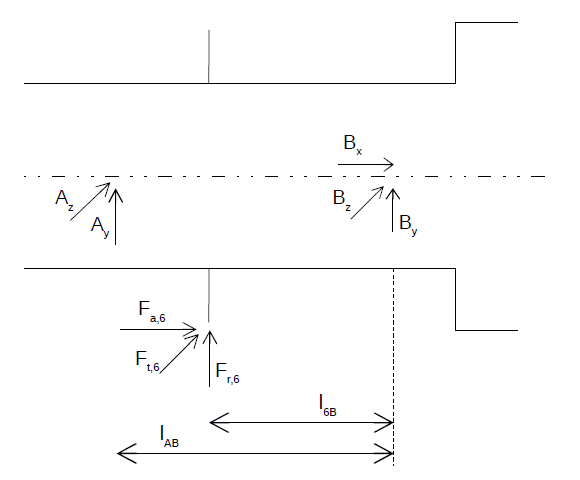
\includegraphics[width=1\textwidth,keepaspectratio]{figures/Gang1Hohl.png}
\end{center}
\[l_{AB} =171\text{ mm} \text{ , } l_{6B} = 128,5\text{ mm}\]
\begin{align*}
	\sum M\textsubscript{y}\textsuperscript{(B)} &\overset{!}{=} 0 = -A_z \x l_{AB} - F_{t,6,1} \x l_{6B} \\
	&\implies A_z = -F_{t,6,1} \x \frac{l_{6B}}{l_{AB}} = -742,68 \text{ N} \\ \\
	\sum M\textsubscript{z}\textsuperscript{(B)} &\overset{!}{=} 0 = -A_y \x l_{AB} - F_{r,6,1} \x l_{6B} + F_{a,6,1} \x \frac{d_6}{2}\\
	&\implies A_y = \frac{-F_{r,6,1} \x l_{6B} + F_{a,6,1} \x \frac{d_6}{2}} {l_{AB}}= -130,9 \text{ N} 
\end{align*}
\newpage
\item Gleichgewichte Welle II:
\begin{center}
	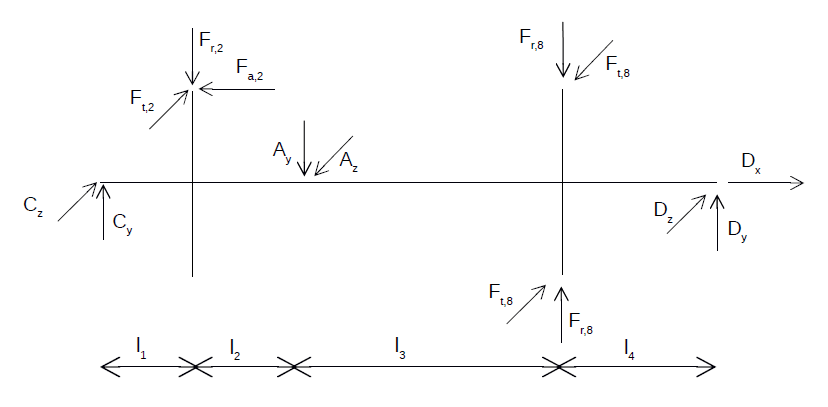
\includegraphics[width=1.04\textwidth,keepaspectratio]{figures/Gang1.png}
\end{center}
\begin{align*}
&l_{1} =269,5\text{ mm} \text{ , } l_{2} = 75,5\text{ mm} \text{ , } l_{3} = 273\text{ mm}  \text{ , } l_{4} = 47\text{ mm} \text{ , } l_{ges} = 665\text{ mm}
\end{align*}
\begin{align*}
	\sum F_x &\overset{!}{=} 0 = -F_{a,2,1} + D_x \implies D_x = F_{a,2,1} = 61,7 \text{ N} \\
	\sum F_y &\overset{!}{=} 0 = C_y - F_{r,2,1}-A_y +D_y - F_{r,8} + F_{r,8}\\ 
	\sum F_z &\overset{!}{=} 0 = A_z - C_z - D_z - F_{t,2,1} + F_{t,8} - F_{t,8}\\ \\
	\sum M\textsubscript{y}\textsuperscript{(D)} &\overset{!}{=} 0 = A_z \x (l_3+l_4)- F_{t,2,1} \x (l_2+l_3+l_4) - C_z \x l_{ges} +l_4 \x F_{t,8}- l_4 \x F_{t,8} \\ 
	&\implies C_z = \frac{(l_3+l_4) \x A_z - F_{t,2,1} \x (l_2+l_3+l_4)}{l_{ges}} = -458,2 \text { N} \\ 
	& \implies D_z = A_z - C_z - F_{t,2,1}= -454 \text{ N}\\ \\
	\sum M\textsubscript{z}\textsuperscript{(D)} &\overset{!}{=} 0 = (l_3+l_4) \x A_y + \frac{d_2}{2} \x F_{a,2,1} + (l_2+l_3+l_4) \x F_{r,2,1}- l_{ges} \x C_y  \\ 
	&\implies C_y = \frac{(l_3+l_4) \x A_y + \frac{d_2}{2} \x F_{a,2,1} + (l_2+l_3+l_4) \x F_{r,2,1}}{l\textsubscript{ges}} = -13,87 \text{ N}\\ 
	& \implies D_y =   A_y - C_y + F_{r,2,1} = -51,38\text{ N}
\end{align*}
\begin{align*}
	C_{x,1} &= \underline{0\text{ N}} & D_{x,1}= \underline{61,7\text{ N}}\\
	C_{y,1} &= \underline{-13,87\text{ N}} & D_{y,1}= \underline{-51,38\text{ N}}\\
	C_{z,1} &= \underline{-458,2\text{ N}} & D_{z,1}= \underline{-454\text{ N}}
\end{align*}
\end{itemize}
\section{Lagerkräfte im Gang 2}
\subsubsection{Berechnung der Zahnradkräfte}
Die Berechnung der Kräfte und die verwendeten Formeln entsprechen dem Kapitel 3.2. Im 2. Gang sind Z1/Z2 und Z4/Z5 im Eingriff.
\begin{itemize}
\item Gegebene Werte: 
	\begin{align*}
	&n_{\mathrm{II},2} = 400\frac{1}{\text{min}} \\
	&T_{\mathrm{II},2,S} = 48,96\text{ Nm} \\
	&d_2 = 217,1\text{ mm} \text{ , } d_4 = 89,4 \text{ mm } 
	\end{align*}
\item Z2, Gang 2:
	\begin{align*} 
	&F_{t,2,2} = \frac{2\x T_{\mathrm{II},2,S}}{d_2} = \frac{2 \x 48,96 \text{ Nm}}{0,2171 \text{ m}} = 451 \text{ N}\\ 
	&F_{r,2,2} = \frac{451 \text{ N} \x \tan{(20^\circ)}}{\cos(20^\circ)} = 174,7\text{ N}\\ 
	&F_{a,2,2} =451 \x \tan(20^\circ) =164,15 \text{ N}
	\end{align*}
\item Z4, Gang 2:
	\begin{align*} 
	&F_{t,4,2} = \frac{2\x T_{\mathrm{II},2,S}}{d_4} = \frac{2 \x 48,96 \text{ Nm}}{0,0894 \text{ m}} = 1095,3 \text{ N}\\ 
	&F_{r,4,2} = \frac{1095,3 \text{ N} \x \tan{(20^\circ)}}{\cos(20^\circ)} = 424,2\text{ N}\\ 
	&F_{a,4,2} =1095,3 \x \tan(20^\circ) =398,7 \text{ N}
	\end{align*}
\end{itemize}
\newpage
\subsubsection{Berechnung der Lagerkräfte}
\begin{itemize}
	\item Gleichgewichte Welle II:
	\begin{center}
		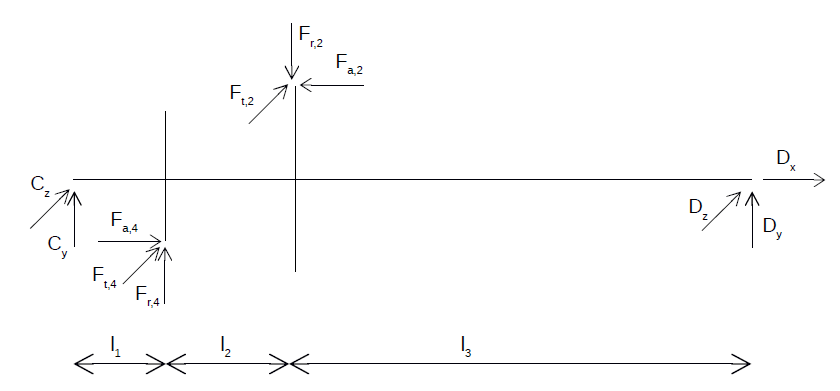
\includegraphics[width=1.04\textwidth,keepaspectratio]{figures/Gang2.png}
	\end{center}
\[l_{1} =118\text{ mm} \text{ , } l_{2} = 151,5\text{ mm} \text{ , } l_{3} = 395,5\text{ mm}  \text{ , } l_{ges} = 665\text{ mm}\]
	\begin{align*}
	\sum F_x &\overset{!}{=} 0 = F_{a,4,2} -F_{a,2,2} + D_x \implies D_x = -F_{a,4,2} +F_{a,2,2}= -234,55 \text{ N} \\
	\sum F_y &\overset{!}{=} 0 = C_y +F_{r,4,2}- F_{r,2,2}+D_y \\ 
	\sum F_z &\overset{!}{=} 0 = - C_z - D_z - F_{t,2,2} - F_{t,4,2} \\ \\
	\sum M\textsubscript{y}\textsuperscript{(D)} &\overset{!}{=} 0 = - F_{t,2,2} \x l_3 - C_z \x l_{ges} -(l_2 + l_3) \x F_{t,4,2} \\ 
	&\implies C_z = \frac{- F_{t,2,2} \x l_3 - (l_2+l_3) \x F_{t,4,2} }{l_{ges}} = -1169,2 \text { N} \\ 
	& \implies D_z = - C_z - F_{t,2,2} - F_{t,4,2}= -377,1 \text{ N}\\ \\
	\sum M\textsubscript{z}\textsuperscript{(D)} &\overset{!}{=} 0 = \frac{d_2}{2} \x F_{a,2,2} + \frac{d_4}{2} \x F_{a,4,2} + l_3 \x F_{r,2,2} - (l_2 + l_3) \x F_{r,4,2}- l_{ges} \x C_y  \\ 
	&\implies C_y = \frac{ \frac{d_2}{2} \x F_{a,2,2} + \frac{d_4}{2} \x F_{a,4,2}  + l_3 \x F_{r,2,2} - (l_2 + l_3) \x F_{r,4,2}}{l\textsubscript{ges}} = -191,6 \text{ N}\\ 
	& \implies D_y =  - C_y - F_{r,4,2} + F_{r,2,2} = -58,1\text{ N}
	\end{align*}
	\begin{align*}
	C_{x,2} &= \underline{0\text{ N}} & D_{x,2}= \underline{-234,55\text{ N}}\\
	C_{y,2} &= \underline{-191,6\text{ N}} & D_{y,2}= \underline{-58,1\text{ N}}\\
	C_{z,2} &= \underline{-1169,2\text{ N}} & D_{z,2}= \underline{-377,1\text{ N}}
	\end{align*}
\end{itemize}
\section{Lagerkräfte im Gang 3}
\subsubsection{Berechnung der Zahnradkräfte}
Die Berechnung der Kräfte und die verwendeten Formeln entsprechen dem Kapitel 3.2. Im 3. Gang sind Z1/Z3 und Z6/Z7 im Eingriff.
\begin{itemize}
	\item Gegebene Werte: 
	\begin{align*}
	&n_{\mathrm{II},3} = \frac{n_{\mathrm{III},3}}{i_{9,8}} = 1600\frac{1}{\text{min}} \\
	&T_{\mathrm{III},3,S} = 121,63\text{ Nm} \\	
	&d_3 = 217,1\text{ mm} \text{ , } d_6 = 149 \text{ mm } 
	\end{align*}
	\item Z3, Gang 3:
	\begin{align*} 
	&F_{t,3,3} = \frac{2\x T_{\mathrm{III},3,S}}{d_3} = \frac{2 \x 121,63 \text{ Nm}}{0,2171 \text{ m}} = 1120,5 \text{ N}\\ 
	&F_{r,3,3} = \frac{1120,5 \text{ N} \x \tan{(20^\circ)}}{\cos(20^\circ)} =434\text{ N}\\ 
	&F_{a,3,3} =1120,5 \x \tan(20^\circ) =407,8 \text{ N}
	\end{align*}
	\item Z6, Gang 3:
	\begin{align*}
	&F_{t,6,3} = \frac{2\x T_{\mathrm{III},3,S}}{d_6} = \frac{2 \x 121,63 \text{ Nm}}{0,149 \text{ m}} = 1632,6\text{ N}\\ 
	&F_{r,6,3} = 1632,6 \text{ N} \x \tan{(20^\circ)} = 632,35\text{ N}\\ 
	&F_{a,6,3} =1632,6\x \tan(20^\circ) =594,2 \text{ N}
	\end{align*}
\end{itemize}
\newpage
\subsubsection{Berechnung der Lagerkräfte}
\begin{itemize}
	\item Momentensummen Hohlwelle:
	\begin{center}
		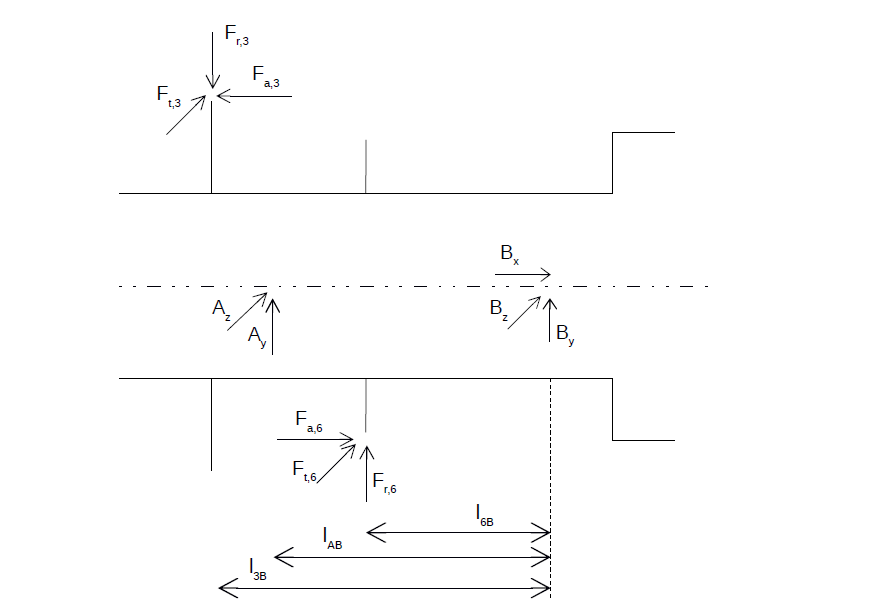
\includegraphics[width=1.2\textwidth,keepaspectratio]{figures/Gang3Hohl.png}
	\end{center}
\[l_{AB} =171\text{ mm} \text{ , } l_{3B} = 175,8\text{ mm} \text{ , } l_{6B} = 128,5\text{ mm}  \]
	\begin{align*}
	\sum M\textsubscript{y}\textsuperscript{(B)} &\overset{!}{=} 0 = -A_z \x l_{AB} - F_{t,6,3} \x l_{6B} - F_{t,3,3} \x l_{3B} \\
	&\implies A_z =  \frac{-F_{t,6,1} \x l_{6B} - F_{t,3,3} \x l_{3B}}{l_{AB}} = -2378,8\text{ N} \\ \\
	\sum M\textsubscript{z}\textsuperscript{(B)} &\overset{!}{=} 0 = -A_y \x l_{AB} - F_{r,6,3} \x l_{6B} + F_{a,6,3} \x \frac{d_6}{2} + F_{a,3,3} \x \frac{d_3}{2} + F_{r,3,3} \x l_{3B}\\
	&\implies A_y = \frac{-F_{r,6,3} \x l_{6B} + F_{a,6,3} \x \frac{d_6}{2} +F_{a,3,3} \x \frac{d_3}{2} + F_{r,3,3} \x l_{3B}} {l_{AB}}= 488,7 \text{ N} 
	\end{align*}
	\newpage
	\item Gleichgewichte Welle II:
	\begin{center}
		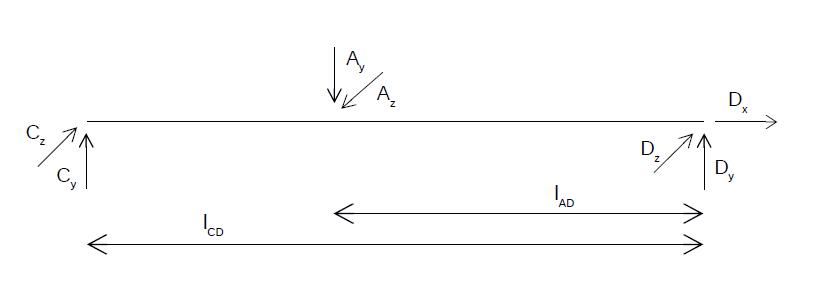
\includegraphics[width=1.04\textwidth,keepaspectratio]{figures/Gang3.png}
	\end{center}
\[l_{AD} =322\text{ mm} \text{ , } l_{CD} = 665\text{ mm} \]
	\begin{align*}
	\sum F_x &\overset{!}{=} 0 =  D_x \implies D_x =  0 \text{ N} \\
	\sum F_y &\overset{!}{=} 0 = C_y -A_y +D_y \\ 
	\sum F_z &\overset{!}{=} 0 = A_z - C_z - D_z\\ \\
	\sum M\textsubscript{y}\textsuperscript{(D)} &\overset{!}{=} 0 = A_z \x l_{AD} - C_z \x l_{CD}\\ 
	&\implies C_z = A_z \x \frac{l_{AD}}{l_{CD}} = -1151,8 \text { N} \\ 
	& \implies D_z = A_z - C_z = -1227 \text{ N}\\ \\
	\sum M\textsubscript{z}\textsuperscript{(D)} &\overset{!}{=} 0 = A_y \x l_{AD} - C_y \x l_{CD} \\ 
	&\implies C_y = A_y \x \frac{l_{AD}}{l_{CD}} = 236,6 \text{ N}\\ 
	& \implies D_y =   A_y - C_y = 252,1\text{ N}
	\end{align*}
	\begin{align*}
	C_{x,3} &= \underline{0\text{ N}} & D_{x,3}= \underline{0\text{ N}}\\
	C_{y,3} &= \underline{236,6\text{ N}} & D_{y,3}= \underline{252,1\text{ N}}\\
	C_{z,3} &= \underline{-1151,8\text{ N}} & D_{z,3}= \underline{-1227\text{ N}}
	\end{align*}
\end{itemize}
\section{Lagerkräfte im Gang 4}
Die Lagerkräfte der Welle 2 im 4. Gang wurden im Kaptel 3.2 zur Berechnung der Schnittkräfte bestimmt.
\begin{align*}
	n_{\mathrm{II},4} &= 1600\frac{1}{\text{min}} \\
	C_{x,4} &= \underline{0\text{ N}} & D_{x,4}= \underline{-581,94\text{ N}}\\
	C_{y,4} &= \underline{327,26\text{ N}} & D_{y,4}= \underline{710,23\text{ N}}\\
	C_{z,4} &= \underline{-2616,8\text{ N}} & D_{z,4}= \underline{-1689,53\text{ N}}
\end{align*}
\section{Berechnung der äquivalenten dynamischen Lagerbelastung}
Die Formeln für die Berechnung stammen aus dem Skript KL III\ccite{bib:poll:kl3} Seite 73 bis 74.
Die Werte für die statische und dynamisch Tragzahl stammen aus dem Tabellenbuch Roloff/Matek \ccite{bib:roloffMatek:tabellenbuch} Seite 205.
\subsection{Gang 1}
\subsubsection{Gang 1, Festlager:} Rillenkugellager , DIN 625-6206\\
\begin{itemize}
	\item gegebene Werte:
	\begin{align*}
	&n_{{\mathord{\mathrm{II}},1}} &&=  400 \frac{1}{\text{min}} \\
	&\text{statische Tragzahl } C_{0} &&= 11200 \text{ N}\\
	&\text{dynamische Tragzahl } C &&= 19300 \text{ N} \\
	&\text{Lebensdauerexponent } p &&= 3 \text{ (für Wälzlager)} \\
	&F_{Dx} && = 61,7 \text{ N}\\
	&F_{Dy} && = -51,38 \text{ N}\\
	&F_{Dz} && = -454 \text{ N}
	\end{align*} 
	\item Berechnung der äquivalenten dynamischen Belastung
	\begin{align*}
	&\text{dynamische radiale Lagerkraft } F_r&& = \sqrt{F_{Dy}^2 + F_{Dz}^2 } = 456,9 \text{ N} \\
	&\text{dynamische axiale Lagerkraft } F_a&& = |F_{Dx}| = 61,7 \text{ N}\\
	&\text{Belastungsfaktor } e &&= 0,22 \text{ da } \frac{F_a}{C_0} < 0,025
	\end{align*} 
	\[\frac{F_a}{F_r} = 0,14 \implies \frac{F_a}{F_r} < e\]
	Deshalb folgt aus Tabelle 2.9 im Skript KL III\ccite{bib:poll:kl3} : X= 1 \text{, } Y= 0 \\
	Die äquivalente dynamische Belastung ergibt sich zu: 
	\[
	P= X \x F_r = 456,9 \text{ N}
	\]
\end{itemize}

\subsubsection{Gang 1, Loslager:} Rillenkugellager, DIN 625-6206\\
\begin{itemize}
	\item gegebene Werte:
	\begin{align*}
	&n_{{\mathord{\mathrm{II}},1}} &&=  400 \frac{1}{\text{min}} \\
	&\text{statische Tragzahl } C_{0} &&= 11200 \text{ N}\\
	&\text{dynamische Tragzahl } C &&= 19300 \text{ N} \\
	&\text{Lebensdauerexponent } p &&= 3 \text{ (für Wälzlager)} \\
	&F_{Cy} && = -13,87 \text{ N}\\
	&F_{Cz} && = -458,2 \text{ N}
	\end{align*} 
	\item Berechnung der äquivalenten dynamischen Belastung
	\begin{align*}
	&\text{dynamische radiale Lagerkraft } F_r&& = \sqrt{F_{Cy}^2 + F_{Cz}^2 } = 458,4 \text{ N} \\
	&\text{dynamische axiale Lagerkraft } F_a&& = F_{Cx} = 0\text{ N}
	\end{align*} 
	Da es sich um eine reine Radialbelastung handelt, ergeben sich der Radial- und Axialfaktor zu: $X= 1$ und $Y=0$\\
	Daraus ergibt sich die äquivalente dynamische Lagerbelastung zu:  
	\[
	P= X \x F_r =458,4 \text{ N}
	\]
\end{itemize}
\newpage

\subsection{Gang 2}
\subsubsection{Gang 2, Festlager:} Rillenkugellager , DIN 625-6206\\
\begin{itemize}
	\item gegebene Werte:
	\begin{align*}
	&n_{{\mathord{\mathrm{II}},2}} &&=  400 \frac{1}{\text{min}} \\
	&\text{statische Tragzahl } C_{0} &&= 11200 \text{ N}\\
	&\text{dynamische Tragzahl } C &&= 19300 \text{ N} \\
	&\text{Lebensdauerexponent } p &&= 3 \text{ (für Wälzlager)} \\
	&F_{Dx} && = -234,55 \text{ N}\\
	&F_{Dy} && = -58,1 \text{ N}\\
	&F_{Dz} && = -377,1 \text{ N}
	\end{align*} 
	\item Berechnung der äquivalenten dynamischen Belastung
	\begin{align*}
	&\text{dynamische radiale Lagerkraft } F_r&& = \sqrt{F_{Dy}^2 + F_{Dz}^2 } = 381,5 \text{ N} \\
	&\text{dynamische axiale Lagerkraft } F_a&& = |F_{Dx}| = 234,55 \text{ N}\\
	&\text{Belastungsfaktor } e &&= 0,37 \text{ da } \frac{F_a}{C_0} = 0,02
	\end{align*}
	\[\frac{F_a}{F_r} = 0,6 \implies \frac{F_a}{F_r} > e\]
	Deshalb folgt aus Tabelle 2.9 im Skript KL III\ccite{bib:poll:kl3} : X= 0,56 \text{, } Y= 1,2 \\
	Die äquivalente dynamische Belastung ergibt sich zu: 
	\[
	P= X \x F_r + Y \x F_a = 495,1 \text{ N}
	\]
\end{itemize}
\newpage
\subsubsection{Gang 2, Loslager:} Rillenkugellager, DIN 625-6206\\
\begin{itemize}
	\item gegebene Werte:
	\begin{align*}
	&n_{{\mathord{\mathrm{II}},2}} &&=  400 \frac{1}{\text{min}} \\
	&\text{statische Tragzahl } C_{0} &&= 11200 \text{ N}\\
	&\text{dynamische Tragzahl } C &&= 19300 \text{ N} \\
	&\text{Lebensdauerexponent } p &&= 3 \text{ (für Wälzlager)} \\
	&F_{Cy} && = -191,6\text{ N}\\
	&F_{Cz} && =-1169,2 \text{ N}
	\end{align*} 
	\item Berechnung der äquivalenten dynamischen Belastung
	\begin{align*}
	&\text{dynamische radiale Lagerkraft } F_r&& = \sqrt{F_{Cy}^2 + F_{Cz}^2 } =1184,8 \text{ N} \\
	&\text{dynamische axiale Lagerkraft } F_a&& = F_{Cx} = 0\text{ N}
	\end{align*} 
	Da es sich um eine reine Radialbelastung handelt, ergeben sich der Radial- und Axialfaktor zu: $X= 1$ und $Y=0$\\
	Daraus ergibt sich die äquivalente dynamische Lagerbelastung zu:  
	\[
	P= X \x F_r =1184,8 \text{ N}
	\]
\end{itemize}
\newpage

\subsection{Gang 3}
\subsubsection{Gang 3, Festlager:} Rillenkugellager , DIN 625-6206\\
\begin{itemize}
	\item gegebene Werte:
	\begin{align*}
	&n_{{\mathord{\mathrm{II}},3}} &&=  1600 \frac{1}{\text{min}} \\
	&\text{statische Tragzahl } C_{0} &&= 11200 \text{ N}\\
	&\text{dynamische Tragzahl } C &&= 19300 \text{ N} \\
	&\text{Lebensdauerexponent } p &&= 3 \text{ (für Wälzlager)} \\
	&F_{Dx} && = 0\text{ N}\\
	&F_{Dy} && = 252,1 \text{ N}\\
	&F_{Dz} && = -1127 \text{ N}
	\end{align*} 
	\item Berechnung der äquivalenten dynamischen Belastung
	\begin{align*}
	&\text{dynamische radiale Lagerkraft } F_r&& = \sqrt{F_{Dy}^2 + F_{Dz}^2 } = 1154,9 \text{ N} \\
	&\text{dynamische axiale Lagerkraft } F_a&& = |F_{Dx}| = 0 \text{ N}
	\end{align*} 
	Da es sich um eine reine Radialbelastung handelt, ergeben sich der Radial- und Axialfaktor zu: $X= 1$ und $Y=0$\\
	Daraus ergibt sich die äquivalente dynamische Lagerbelastung zu:  
	\[
	P= X \x F_r =1154,9 \text{ N}
	\]
\end{itemize}
\newpage
\subsubsection{Gang 3, Loslager:} Rillenkugellager, DIN 625-6206\\
\begin{itemize}
	\item gegebene Werte:
	\begin{align*}
	&n_{{\mathord{\mathrm{II}},3}} &&=  1600 \frac{1}{\text{min}} \\
	&\text{statische Tragzahl } C_{0} &&= 11200 \text{ N}\\
	&\text{dynamische Tragzahl } C &&= 19300 \text{ N} \\
	&\text{Lebensdauerexponent } p &&= 3 \text{ (für Wälzlager)} \\
	&F_{Cy} && = 236,6 \text{ N}\\
	&F_{Cz} && = -1151,8 \text{ N}
	\end{align*} 
	\item Berechnung der äquivalenten dynamischen Belastung
	\begin{align*}
	&\text{dynamische radiale Lagerkraft } F_r&& = \sqrt{F_{Cy}^2 + F_{Cz}^2 } =1175,8 \text{ N} \\
	&\text{dynamische axiale Lagerkraft } F_a&& = F_{Cx} = 0\text{ N}
	\end{align*} 
	Da es sich um eine reine Radialbelastung handelt, ergeben sich der Radial- und Axialfaktor zu: $X= 1$ und $Y=0$\\
	Daraus ergibt sich die äquivalente dynamische Lagerbelastung zu:  
	\[
	P= X \x F_r =1175,8 \text{ N}
	\]
\end{itemize}
\newpage

\subsection{Gang 4}
\subsubsection{Gang 4, Festlager:} Rillenkugellager , DIN 625-6206\\
\begin{itemize}
	\item gegebene Werte:
	\begin{align*}
	&n_{{\mathord{\mathrm{II}},4}} &&=  1600 \frac{1}{\text{min}} \\
	&\text{statische Tragzahl } C_{0} &&= 11200 \text{ N}\\
	&\text{dynamische Tragzahl } C &&= 19300 \text{ N} \\
	&\text{Lebensdauerexponent } p &&= 3 \text{ (für Wälzlager)} \\
	&F_{Dx} && = -581,94 \text{ N}\\
	&F_{Dy} && = 710,23 \text{ N}\\
	&F_{Dz} && = -1689,53 \text{ N}
	\end{align*} 
	\item Berechnung der äquivalenten dynamischen Belastung
	\begin{align*}
	&\text{dynamische radiale Lagerkraft } F_r&& = \sqrt{F_{Dy}^2 + F_{Dz}^2 } =1832,7\text{ N} \\
	&\text{dynamische axiale Lagerkraft } F_a&& = |F_{Dx}| = 581,94 \text{ N}\\
	&\text{Belastungsfaktor } e &&= 0,24 \text{ da } \frac{F_a}{C_0} = 0,05
	\end{align*} 
	\[\frac{F_a}{F_r} = 0,32 \implies \frac{F_a}{F_r} > e\]
	Deshalb folgt aus Tabelle 2.9 im Skript KL III\ccite{bib:poll:kl3} : X= 0,56 \text{, } Y= 1,8 \\
	Die äquivalente dynamische Belastung ergibt sich zu: 
	\[
	P= X \x F_r + Y \x F_a= 2073,8 \text{ N}
	\]
\end{itemize}
\newpage
\subsubsection{Gang 4, Loslager:} Rillenkugellager, DIN 625-6206\\
\begin{itemize}
	\item gegebene Werte:
	\begin{align*}
	&n_{{\mathord{\mathrm{II}},2}} &&=  1600 \frac{1}{\text{min}} \\
	&\text{statische Tragzahl } C_{0} &&= 11200 \text{ N}\\
	&\text{dynamische Tragzahl } C &&= 19300\text{ N} \\
	&\text{Lebensdauerexponent } p &&= 3 \text{ (für Wälzlager)} \\
	&F_{Cy} && = 327,26 \text{ N}\\
	&F_{Cz} && = -2616,8 \text{ N}
	\end{align*} 
	\item Berechnung der äquivalenten dynamischen Belastung
	\begin{align*}
	&\text{dynamische radiale Lagerkraft } F_r&& = \sqrt{F_{Cy}^2 + F_{Cz}^2 } =2637,2 \text{ N} \\
	&\text{dynamische axiale Lagerkraft } F_a&& = F_{Cx} = 0\text{ N}
	\end{align*} 
	Da es sich um eine reine Radialbelastung handelt, ergeben sich der Radial- und Axialfaktor zu: $X= 1$ und $Y=0$\\
	Daraus ergibt sich die äquivalente dynamische Lagerbelastung zu:  
	\[
	P= X \x F_r =2637,2\text{ N}
	\]
\end{itemize}
\newpage

\section{Bestimmung der Lastkollektive und der Lebensdauer}
Die Formeln für die Berechnung stammen aus dem Skript KL III\ccite{bib:poll:kl3} Seite 76
\subsubsection{Lastkollektiv Festlager}
\begin{align*}
	n_m =& n_{\mathord{\mathrm{II}},1} \x \frac{40 \%}{100 \%} + n_{\mathord{\mathrm{II}},2} \x \frac{25 \%}{100 \%} + n_{\mathord{\mathrm{II}},3} \x \frac{20 \%}{100 \%} + n_{\mathord{\mathrm{II}},4} \x \frac{15 \%}{100 \%} \\
	n_m =& 400 \frac{1}{\text{min}} \x 0,4 + 400 \frac{1}{\text{min}} \x 0,25 +1600 \frac{1}{\text{min}} \x 0,2 + 1600 \frac{1}{\text{min}} \x 0,15 = 820 \frac{1}{\text{min}} \\
	P_{\text{äq}} =& \sqrt[p]{P_1 ^{p} \x \frac{n_1}{n_m} \x \frac{q_1}{100\% } + P_2 ^{p} \x \frac{n_2}{n_m} \x \frac{q_2}{100 \%} + P_3 ^{p} \x \frac{n_3}{n_m} \x \frac{q_3}{100\% } + P_4 ^{p} \x \frac{n_4}{n_m} \x \frac{q_4}{100 \%}} \\
	=& \sqrt[3]{(456,9 \text{ N}) ^{3} \x \frac{400}{820} \x \frac{40 \%}{100 \%} +(495,1 \text{ N} )^{3} \x \frac{400}{820} \x \frac{25 \%}{100\% }+(1154,9 \text{ N} )^{3} \x \frac{1600}{820} \x \frac{20 \%}{100\% }+} \\ &\overline{(2073,8 \text{ N} )^{3} \x \frac{1600}{820} \x \frac{15 \%}{100\% }} \\
	=& 1480,47 \text{ N}
\end{align*}
\subsubsection{Lastkollektiv Loslager}
\begin{align*}
	n_m =& n_{\mathord{\mathrm{II}},1} \x \frac{40 \%}{100 \%} + n_{\mathord{\mathrm{II}},2} \x \frac{25 \%}{100 \%} + n_{\mathord{\mathrm{II}},3} \x \frac{20 \%}{100 \%} + n_{\mathord{\mathrm{II}},4} \x \frac{15 \%}{100 \%} \\
	n_m =& 400 \frac{1}{\text{min}} \x 0,4 + 400 \frac{1}{\text{min}} \x 0,25 + 1600 \frac{1}{\text{min}} \x 0,2 + 1600 \frac{1}{\text{min}} \x 0,15 = 820 \frac{1}{\text{min}} \\
	P_{\text{äq}} =& \sqrt[p]{P_1 ^{p} \x \frac{n_1}{n_m} \x \frac{q_1}{100\% } + P_2 ^{p} \x \frac{n_2}{n_m} \x \frac{q_2}{100 \%} +P_3 ^{p} \x \frac{n_3}{n_m} \x \frac{q_3}{100\% } + P_4 ^{p} \x \frac{n_4}{n_m} \x \frac{q_4}{100 \%}} \\
	=& \sqrt[3]{(458,4 \text{ N}) ^{3} \x \frac{400}{820} \x \frac{40 \%}{100 \%} +(1184,8 \text{ N} )^{3} \x \frac{400}{820} \x \frac{25 \%}{100\% }+(1175,8 \text{ N} )^{3} \x \frac{1600}{820} \x \frac{20 \%}{100\% } +}\\
	&\overline{(2637,2 \text{ N} )^{3} \x \frac{1600}{820} \x\frac{15 \%}{100\% }} \\
	=& 1839,47 \text{ N}
\end{align*}
\newpage
\subsubsection{Lebensdauer Festlager}
$L_{10h}= \left( \frac{C}{P_{\text{äq}}} \right) ^p \x \frac{10^6}{n_m \x 60} = \left( \frac{19300 \text{ N}}{1614,2 \text{ N}} \right) ^3 \x \frac{10^6}{500 \frac{1}{\text{min}} \x 60} = 45030,6 \text{ h} = 5,1 \text{ a}$

\subsubsection{Lebensdauer Loslager}
$L_{10h}= \left( \frac{C}{P_{\text{äq}}} \right) ^p \x \frac{10^6}{n_m \x 60} = \left( \frac{19300 \text{ N}}{2087,7 \text{ N}} \right) ^3 \x \frac{10^6}{500 \frac{1}{\text{min}} \x 60} = 23476,2 \text{ h} = 2,7 \text{ a}$
	\chapter{Schwachstellenberechnung}
\section{Berechnung Welle-Nabe-Verbindungen}
In diesem Kapitel wird die maximale Flächenpressung für jede Passfederverbindung berechnet. Dieses wird anschließend mit der durch den Werkstoff vorgegebenen zulässigen Pressung verglichen. Als Sicherheitsfaktor wird S=1,5 gewählt.\\
\begin{itemize}
	\item Zulässige Flächenpressung \hfill  (Skript KL IV\ccite{bib:poll:kl4} S. 56)
	\begin{align*}
		\text{Werkstoff C45: } &R_{e,min} = 430 \frac{\text{N}}{\text{mm}^2} \text{ bei } d\le 40 \text{ mm} \\
		 &R_{e,min} = 370 \frac{\text{N}}{\text{mm}^2} \text{ bei } d> 40 \text{ mm} \\
		 &p_{zul} = 0,9 \x R_{e,min}  \\
		 &p_{zul} = 387 \frac{\text{N}}{\text{mm}^2} \text{ für } d\le 40 \text{ mm} \\
		  &p_{zul} = 330 \frac{\text{N}}{\text{mm}^2} \text{ für } d> 40 \text{ mm} \\
	\end{align*}
	\item maximale Flächenpressung \hfill (Skript KL IV\ccite{bib:poll:kl4} S. 55 - 56)
	\begin{align*}
		&p_m = \frac{2 \x c_B \x T}{d \x h' \x l' \x n \x \phi} && \\
		&\text{für alle Passfedern gilt: } &n=1 & \\
		& &\phi = 1& \\
		& &c_B = 1 &\text{ (leichte Stöße, Tabelle 3.2 aus Skript KL IV)}\\
		& l' = l - b \text{ wenn } l'\le 1,2 \x d &&\implies \text{sonst setze } l' = 1,2 \x d \\
		&h' = 0,45 \x h &&\\
	\end{align*}
	Als Beispiel wird Passfeder 2 (Positionsnummer 39) auf Welle II berechnet:
	\begin{align*}
		&M= 1,5 \x T_{\mathord{\mathrm{II}},4,S} = 1,5 \x  71,47\text{ Nm} = 107,21 \text{ Nm} \\
		&d= 35 \text{ mm} \\
		&l= 22 \text{ mm} \\
		&h= 8 \text{ mm} \\
		&b= 10 \text{ mm} \\
		&l'= 12 \text{ mm} \\
		&h'= 3,6 \text{ mm} \\ \\
		&\implies p_m = \frac{2 \x 1,1 \x 107210 \text{ Nmm}}{35 \text{ mm} \x 3,6 \text{ mm} \x 12 \text{ mm} \x 1 \x 1}  = 155,99 \frac{\text{N}}{\text{mm}^2}\\
		& p_m < p_{zul} = 387 \frac{\text{N}}{\text{mm}^2} \\
	\end{align*}
	Als weiteres Beispiel wird die Passfeder 1 (Positionsnummer 15) auf Welle I berechnet, da hier je nachdem, welche Zahnräder im Eingriff sind, unterschiedliche Längen der Passfeder beansprucht werden:
	\begin{align*}
	&d= 30 \text{ mm} &\\
	&h= 7 \text{ mm} &\\
	&b= 8 \text{ mm} &\\
	&h'= 3,15 \text{ mm}& \\ \\
	&\text{Z1/Z2:} &&l_1 = 40 \text{ mm, } l_1' = 32 \text{ mm}\\
	& && M_1 = 1,5 \x T_{\mathord{\mathrm{I}},2,S} = 1,5 \x 16,32 \text{ Nm} =24,48 \text{ Nm} \\
	& &&\implies p_{m,1} = 17,8\frac{\text{N}}{\text{mm}^2} \\ \\
	&\text{Z1/Z3:} &&l_2 = 54\text{ mm, } l_2' = 46 \text{ mm}\\
	& && M_2 = 1,5 \x T_{\mathord{\mathrm{I}},4,S} = 1,5 \x 95,29 \text{ Nm} = 142,94 \text{ Nm}\\
	& &&\implies p_{m,2} = 72,3\frac{\text{N}}{\text{mm}^2} \\
	\end{align*}
\end{itemize}
\newpage
Alle weiteren Werte der Passfederberechnung sind in der folgenden Tabelle dargestellt. Alle Längen werden in der Einheit Millimeter angegeben. \\ \\
\begin{tabular}{|c|c|c|c|c|c|c|c|c|c|c|c|}\hline
	 Passfeder & Pos. Nr. &Welle & d & l & b & h & l' & h' & T(Nm) & $p_m(\frac{\text{N}}{\text{mm}^2})$ \\ \hline \hline
	 1, bei $Z_1$(Eingriff Z2) & 19 & $\mathrm{I}$ &30 & 40 & 8 & 7 & 32 & 3,15 & 24,28 & 17,8 \\ \hline
	 1, bei $Z_1$(Eingriff Z2) & 19 & $\mathrm{I}$ &30 & 54 & 8 & 7 & 46 & 3,15 & 142,94 & 72,3 \\ \hline
	 2, bei $Z_4$ & 39 &$\mathrm{II}$ & 35 & 22 & 10 & 8 & 12 & 3,6 & 107,21 & 155,99 \\ \hline
	 3, bei $Z_2$ & 102 &$\mathrm{II}$ & 42 & 32 & 12 & 8 & 20 & 3,6 & 107,21 & 78 \\ \hline
	4, bei $Z_8$ & 39 &$\mathrm{II}$ & 35 & 22 & 10 & 8 & 12 & 3,6 & 107,21 & 155,99 \\ \hline
	5, bei Kupplung & 127 & $\mathrm{IV}$ & 55 & 28 & 16 & 10 & 66 & 4,5 & 268,99 & 36,23 \\ \hline
	 6, bei Kupplung & 118 &$\mathrm{IV}$ & 85 & 20 & 12 & 8 & 8 & 3,6 & 268,99 & 241,74 \\ \hline
	 7, bei $Z_{11}$ & 75 &$\mathrm{V}$ & 40 & 28 & 12 & 8 & 16 & 3,6 & 268,99 & 256,85 \\ \hline
	 8, bei $Z_{12}$ & 94 &$\mathrm{VI}$ & 40 & 28 & 12 & 8 & 16 & 3,6 & 268,99 & 256,85 \\ \hline
\end{tabular} \\
\vspace{.5cm}
\\ Da bei allen Passfedern gilt $p_m < p_{zul}$ halten die Passfedern der Belastung stand.
	\newpage
\section{Berechnung der Schraubenverbindungen}
\subsection{Verschraubung Lagerdeckel}
Da an allen Festlagern dieselben Schrauben verwendet wurden, muss nur die Schraubenverbindung mit der höchsten Belastung berechnet werden. Diese ergibt sich durch die Axialkraft, die auf die jeweilige Welle wirkt. Aufgrund der Axialkraft der Kegelräder ist die Welle V am Höchsten belastet.
Aus diesen Gründen wird im Folgenden die Schraubenverbindung des Lagerdeckels am Festlager der Welle V berechnet.
\subsubsection{\underline{Kräfte}}
\[
	F_A = F_{a,11} = 1381,81 \text{ N}
\]
\flushleft
Betriebskraft pro Schraube: $F_B = \frac{F_A}{Z} = \frac{1381,81 \text{ N}}{4} = 345,45 \text{ N}$ \\
Vorspannungsverhältnis soll im Bereich $\frac{F_V}{F_B} = 2,5...3,5$ liegen (siehe Skript KL IV \ccite{bib:poll:kl4} Seite 37). \\
\vspace{.5cm}
Wähle Faktor 2,5 $\implies F_V = 2,5 \x F_B = 863,63 \text{ N}$

\newpage
\subsubsection{\underline{Schraubendaten}}
Sechskantschraube M5x25 nach DIN EN ISO 4014, Festigkeitsklasse 8.8\\
$R_m = 800 \frac{\text{N}}{\text{mm}^2}$\\
$R_e = 8\x8\x10\frac{\text{N}}{\text{mm}^2} = 640 \frac{\text{N}}{\text{mm}^2}$\\
\begin{align*}
\text{Nenndurchmesser: } d &= 5\text{ mm}\\
\text{Nennquerschnitt: } A_N &= \frac{\pi\x d^2}{4} = 19,63\text{ mm}^2\\
\text{Steigung: } P &= 0,8\text{ mm}\\
\text{Flankendurchmesser: } d_2 &= 4,48\text{ mm}\\
\text{Kerndurchmesser: } d_3 &= 4,02 \text{ mm}\\
\text{Flankenwinkel: } \beta &= 60^{\circ}\\
\text{Kernquerschnitt: } A_3 &= \frac{\pi\x d_3^2}{4} = 12,69\text{ mm}^2\\
\text{Spannungsquerschnitt: } A_S &= 14,2 \text{ mm}^2\\
\text{Schlüsselweite: } S &= 8 \text{ mm}\\
\text{Durchmesser Durchgangsbohrung: } D_B &= 5,5 \text{ mm} \text{ (DIN EN 20273)}
\end{align*}
\newpage

\subsubsection{\underline{Vorspannen}}
Formeln und Anhang aus dem Skript KL IV \ccite{bib:poll:kl4} (Seite 37 bis 39, Reibwerte aus A.1.5 und A.1.6) \\
\textbf{Anzugsmoment}\\
\begin{itemize}
		\item Bestimmung Gewindereibmoment: 
		\begin{align*}
		M_{RG} &= F_U \x \frac{d_2}{2} = F_V\x \frac{d_2}{2}\x \tan\left(\phi + p'\right)\\
		\tan\left(\phi\right) &= \frac{P}{d_2 \x \pi}\implies \phi = 3,25^{\circ}\\
		\tan\left(p'\right) &= \frac{\mu_G}{\cos\left(\frac{\beta}{2}\right)} \text{ mit } \mu_G = 0,14 \implies p' = 9,18^{\circ}
		\end{align*}
		\[\implies \text{einsetzen liefert: }  M_{RG} =0,4264 \text{ Nm} = 426,4\text{ Nmm}\]
			
		\item Bestimmung Kopfreibmoment:
		\begin{align*}
		M_{RK}&= F_V\x \mu_K\x \frac{d_R}{2} \text{ mit }\mu_K = 0,14\\
		d_R &= \frac{S+D_B}{2} = 6,75 \text{ mm}
		\end{align*}
		\[\implies \text{einsetzen liefert: }  M_{RK} = 0,4081 \text{ Nm} = 408,1\text{ Nmm} \]
		
		\item Gesamtanzugsmoment:
	$M_A = M_{RG} + M_{RK} = 834,5 \text{ Nmm}$
\end{itemize}
\newpage
\textbf{Spannungen beim Vorspannen}
\begin{itemize}
	\item maximale Schubspannung:
	\begin{align*}
		\tau_{t,V} &= \frac{M_{RG}}{W_p}\\
		W_p &= \frac{\pi\x d_3^3}{16} = 12,76 \text{ mm}^3
	\end{align*}
	\[\implies \tau_{t,V} = 33,42 \frac{\text{N}}{\text{mm}^2}\]
	\item Bestimmung Zugspannung: \\
	\begin{center} $\sigma_{Z,V} = \frac{F_V}{A_S} = 60,82 \frac{\text{N}}{\text{mm}^2}$\end{center}
	\item Berechnung der resultierenden Vergleichsspannung:\\
	\begin{center}
		$\sigma_{v,V} = \sqrt{\sigma_{Z,V}^2+3\x\tau_{t,V}^2} = 83,96 \frac{N}{mm}^2$ \\
	\end{center} 
	Die Sicherheit der Schraubenverbindung gegen plastische Verformung beträgt:\\ 
	\[S_F = \frac{R_{p0,2}}{\sigma_{v,V}} = 7,6\]
\end{itemize}
\newpage
\subsubsection{\underline{unter Betriebslast}}
Formeln aus dem Skript KL IV \ccite{bib:poll:kl4} Seite 41 bis 43 \\
\textbf{Kräfte}
\begin{itemize}
	\item Nachgiebigkeit der Schraube:
	\[\delta_S = \frac{1}{E}\x \left(\frac{1}{d}+\frac{l_1}{A_N}+\frac{l_2}{A_S}\right)\]
	\[\text{mit } E = 2,1\x 10^5 \frac{\text{N}}{\text{mm}^2} \text{, } l_1 = 9 \text{ mm, } l_2 = 16 \text{ mm}\]
	\[\implies \delta_S = 8,5\x 10^{-6} \frac{\text{mm}}{\text{N}}\]
	\item Bestimmung der Nachgiebigkeit der verspannten Elemente nach Fall b)
	\[\alpha = 0,1 \text{ für Stahl, } D_A = 15 \text{ mm, } l_K = 25 \text{ mm, }  d_K = 6,88 \text{ mm}\]
	\begin{align*}
	\delta_H &= \frac{l_K}{E\x A_{ers}}\\
	\text{mit } A_{ers} = \frac{\pi}{4}\x \left(d_K^2 -D_B^2\right) &+ \frac{\pi}{8}\x\left(\frac{D_A}{d_K}-1\right)\x\left(\frac{d_K\x l_K}{5}+ \alpha^2\x l_K^2\right) = 32,26 \text{ mm}^2\\
	\implies \delta_H &= 3,69\x 10^{-6} \frac{\text{mm}}{\text{N}}
	\end{align*}
	Damit ergibt sich die Schraubenkraft unter Betriebslast zu: \\
	\begin{center}
		$F_S = F_V+ \frac{F_B}{1+\frac{\delta_S}{\delta_H}} = 968,2 \text{ N}$
	\end{center}
	Die verbleibende Klemmkraft beträgt dann $ F_{Kl} = F_S-F_B = 622,75 \text{ N}$
\end{itemize}
\newpage
\textbf{Spannungen}
\begin{itemize}
	\item Zugspannung:
	$\sigma_{Z,B} = \frac{F_S}{A_S} = 68,18 \frac{\text{N}}{\text{mm}^2}$\\
	\item Torsionsspannung:\\
	\vspace{0.3cm}
	Das Torsionsmoment im Betrieb hat die Größe des kleineren Wertes von $M_{RK}$ und $M_{RG}$, also: 
	\[\tau_{t,B} = \frac{M_{RK}}{W_p} = 31,98 \frac{\text{N}}{\text{mm}^2}\]
	\item resultierende Vergleichsspannung: $\sigma_{v,B} = \sqrt{\sigma_{Z,B}^2+3\x \tau_{t,B}^2} = 87,8 \frac{N}{mm}^2$\\
	\vspace{.5cm}
	Daraus ergibt sich die Sicherheit der Verbindung gegen plastische Verformung zu: 
	\begin{center}
		$S_F = \frac{R_{p0,2}}{\sigma_{v,B}} = 7,29$
	\end{center}
	Die Schraubenverbindung hält der Belastung also stand.
\end{itemize}
	\chapter{Passungsberechnung}
\flushleft
In diesem Kapitel werden 5 verschiedene Passungen ausgewählt und berechnet. Bei den Toleranzen der Wälzlager wird die Genauigkeitsklasse P0 aus dem LFD Produktkatalog\ccite{bib:www:LFD_Produktkatalog} Seite 27 berücksichtigt.
\begin{align*}
	&N : \text{Nennmaß} \\
	&T : \text{Grundtoleranz} \\
	&A_U : \text{unteres Abmaß} \\
	&A_O : \text{oberes Abmaß} \\
	&G_U : \text{Mindestmaß} \\
	&G_O : \text{Höchstmaß} \\
	&P_U : \text{Mindestpassung} \\
	&P_O : \text{Höchstpassung} \\
\end{align*}
Die verwendeten Formeln stammen aus dem Skript KL I\ccite{bib:lachmayer:kl1} S. 39
\begin{align*}
	&A_U + T = A_O \\
	&G_O = N + A_O \\
	&G_U = N - A_U \\
	&P_O = G_{oB} - G_{uW}\\
	&P_U = G_{uB} - G_{oW}\\
\end{align*}
Die jeweiligen Werte von $T$, $A_O$ und $A_U$ stammen aus dem Tabellenbuch Metall\ccite{bib:fischer:tabellenbuchMetall} Seite 103 bis 105. 
\newpage
\subsubsection{Passung 1: Lageraußenring Rillenkugellager (Festlager, Welle I) und Lagertopf}

Bei dieser Passung wird eine Spielpassung gewählt. Es handelt sich zwar um ein Festlager, der Außenring wird allerdings nur auf Punktlast beansprucht, weshalb keine feste Passung notwendig ist. Außerdem darf nur ein Ring des Lagers fest angepasst werden (das wäre in diesem Fall der Innenring), da das Lager ansonsten nicht mehr zu montieren wäre. \\ 
Passung: J6 (Empfehlung Produktkatalog\ccite{bib:www:LFD_Produktkatalog} Seite 21)
\begin{itemize}
	\item Toleranz Außenring ("Welle"): 47 P0 
	\begin{align*}
	&\text{oberes Abmaß } A_o = 0 \mu\text{m} \\
	&\text{unteres Abmaß } A_u = -11 \mu\text{m} \\
	&G_o = 47 \text{ mm} \\
	&G_u = 46,989 \text{ mm}\\
	\end{align*} 
	\item Toleranz Lagertop ("Bohrung"): 47 J6
	\begin{align*}
	&\text{Toleranzgrad 6 } \implies \text{Grundtoleranz } T=16 \mu\text{m} \\
	&\text{oberes Abmaß } A_o = +24 \mu\text{m} \\
	&A_o = +0,024 \text{ mm} \\
	&A_u = +0,008 \text{ mm} \\
	&G_o = 47,024 \text{ mm} \\
	&G_u = 47,008 \text{ mm}\\
	\end{align*} 
	\item Passungsart
	\begin{align*}
	&P_o = 47,024 \text{ mm} - 46,989 \text{ mm} = +0,035 \text{ mm} \\
	&P_u =47,008 \text{ mm} - 47 \text{ mm} = +0,008 \text{ mm}\\
	&\implies \text{Es liegt in jedem Fall Spiel vor.}
	\end{align*} 
\end{itemize}
\newpage

\subsubsection{Passung 2: Lagerinnenring Rillenkugellager (Festlager) und Welle I}

Bei dieser Passung wird eine Übermaßpassung gewählt. Es handelt sich um ein Festlager, bei dem der Innenring auf Umfangslast beansprucht wird. Deshalb ist eine feste Passung notwendig. \\ 
Passung: k6 (Empfehlung Produktkatalog\ccite{bib:www:LFD_Produktkatalog} Seite 21)
\begin{itemize}
	\item Toleranz Welle: 25 k6
	\begin{align*}
	&\text{Toleranzgrad 6 } \implies \text{Grundtoleranz } T=13 \mu\text{m} \\
	&\text{unteres Abmaß } A_u = +2 \mu\text{m} \\
	&A_u = +0,002 \text{ mm} \\
	&A_o = +0,015 \text{ mm} \\
	&G_u = 25,002 \text{ mm} \\
	&G_o = 25,015 \text{ mm}\\
	\end{align*} 
	\item Toleranz Bohrung: 25 P0 
	\begin{align*}
	&\text{oberes Abmaß } A_o = 0 \mu\text{m} \\
	&\text{unteres Abmaß } A_u = -10 \mu\text{m} \\
	&G_o = 25 \text{ mm} \\
	&G_u = 24,990 \text{ mm}\\
	\end{align*} 
	\item Passungsart
	\begin{align*}
	&P_o = 25 \text{ mm} - 25,002 \text{ mm} = -0,002 \text{ mm} \\
	&P_u = 24,990 \text{ mm} - 25,015 \text{ mm} =-0,025 \text{ mm}\\
	&\implies \text{es liegt in jedem Fall ein Übermaß vor}
	\end{align*} 
\end{itemize}
\newpage

\subsubsection{Passung 3: Lageraußenring Rillenkugellager (Loslager, Welle I) und Lagertopf}

Für die Passung des Loslagers wird eine Spielpassung gewählt. Bei eventueller thermischer Ausdehnung der Welle musss sich der Außenring des Lagers verschieben können, weshalb in jedem Fall Spiel vorliegen muss. \\ 
Passung: G7 (Empfehlung Produktkatalog\ccite{bib:www:LFD_Produktkatalog} Seite 21)
\begin{itemize}
	\item Toleranz Außenring ("Welle"): 62 P0 
	\begin{align*}
	&\text{oberes Abmaß } A_o = 0 \mu\text{m} \\
	&\text{unteres Abmaß } A_u = -13 \mu\text{m} \\
	&G_o = 62 \text{ mm} \\
	&G_u = 61,987 \text{ mm}\\
	\end{align*} 
	\item Toleranz Lagertop ("Bohrung"): 62 G7
	\begin{align*}
	&\text{Toleranzgrad 7 } \implies \text{Grundtoleranz } T=30 \mu\text{m} \\
	&\text{unteres Abmaß } A_u = +10 \mu\text{m} \\
	&A_o = +0,040 \text{ mm} \\
	&A_u = +0,010 \text{ mm} \\
	&G_o = 62,040 \text{ mm} \\
	&G_u = 62,010 \text{ mm}\\
	\end{align*} 
	\item Passungsart
	\begin{align*}
	&P_o = 62,040 \text{ mm} - 61,987 \text{ mm} = +0,053 \text{ mm} \\
	&P_u =62,010 \text{ mm} - 62 \text{ mm} = +0,010 \text{ mm}\\
	&\implies \text{Es liegt in jedem Fall Spiel vor.}
	\end{align*} 
\end{itemize}
\newpage


\subsubsection{Passung 4: Gleitlagerbuchse (Festlager, Schaltwelle 1) und Lagertopf}

An dem Außenring der Gleitlagerbuchse ist eine feste Passung notwendig, das das Lager über eine Presspassung im Gehäuse montiert wird. \\ 
Passung: H7/s6
\begin{itemize}
	\item Toleranz Welle: 21 s6
	\begin{align*}
	&\text{Toleranzgrad 6 } \implies \text{Grundtoleranz } T=13 \mu\text{m} \\
	&\text{unteres Abmaß } A_u = +43\mu\text{m} \\
	&A_u = +0,043 \text{ mm} \\
	&A_o = +0,056 \text{ mm} \\
	&G_u = 21,043 \text{ mm} \\
	&G_o = 21,056 \text{ mm}\\
	\end{align*} 
	\item Toleranz Bohrung: 21 H7
	\begin{align*}
	&\text{Toleranzgrad 7 } \implies \text{Grundtoleranz } T=21 \mu\text{m} \\
	&\text{unteres Abmaß } A_u = 0 \mu\text{m} \implies G_u = N\\
	&A_u = 0 \text{ mm} \\
	&A_o = 0,021 \text{ mm} \\
	&G_u = 21 \text{ mm} \\
	&G_o = 21,021 \text{ mm}\\
	\end{align*} 
	\item Passungsart
	\begin{align*}
	&P_o = 21,021 \text{ mm} - 21,043 \text{ mm} = -0,022 \text{ mm} \\
	&P_u = 21 \text{ mm} - 21,056 \text{ mm} = -0,056 \text{ mm}\\
	&\implies \text{es liegt in jedem Fall ein Übermaß vor}
	\end{align*} 
\end{itemize}
\newpage

\subsubsection{Passung 5: Zahnrad 4 und Welle II}

Da das Zahnrad per Hand auf die Welle aufgeschoben wird, wird für diese Passung ein geringes Passungsspiel gewählt. \\ 
Passung: H7/h6
\begin{itemize}
	\item Toleranz Welle: 35 h6
	\begin{align*}
	&\text{Toleranzgrad 6 } \implies \text{Grundtoleranz } T=16 \mu\text{m} \\
	&\text{oberes Abmaß } A_o = 0\mu\text{m} \implies G_o = N\\
	&A_o = 0 \text{ mm} \\
	&A_u = -0,016 \text{ mm} \\
	&G_o = 35 \text{ mm} \\
	&G_u = 34,984 \text{ mm}\\
	\end{align*} 
	\item Toleranz Bohrung: 35 H7
	\begin{align*}
	&\text{Toleranzgrad 7 } \implies \text{Grundtoleranz } T=25 \mu\text{m} \\
	&\text{unteres Abmaß } A_u = 0 \mu\text{m} \implies G_u = N\\
	&A_u = 0 \text{ mm} \\
	&A_o = 0,025 \text{ mm} \\
	&G_u = 35 \text{ mm} \\
	&G_o = 35,025 \text{ mm}\\
	\end{align*} 
	\item Passungsart
	\begin{align*}
	&P_o = 35,025 \text{ mm} - 34,984 \text{ mm} = 0,041 \text{ mm} \\
	&P_u = 35 \text{ mm} - 35 \text{ mm} =0 \text{ mm}\\
	&\implies \text{ein Verschieben des Zahnrades per Hand ist gerade noch möglich}
	\end{align*} 
\end{itemize}



	
	
	
	% Inhalt Ende
	
	% Glossar
	\printglossary[numberedsection,style=altlist,nonumberlist,title=Glossar]
	
	% Abkürzungsverzeichnis
	\glstoctrue
	\printglossary[type=\acronymtype,style=myListStyle,title=Abkürzungsverzeichnis]
	
%	% Abbildungsverzeichnis
%	\listoffigures
%	\newpage
%	
%	% Tabellenverzeichnis
%	\listoftables
%	\newpage
%	
%	\listofcodes
%	\newpage
	
	% Quellen (Bibliografie)
	\chapter{Quellen}
	\printbibliography[heading=Literatur,nottype=online]
	\printbibliography[heading=Internet,type=online]
	% Anhang (Appendix)
	\cleardoublepage
	\appendix
	\chapter{Anhang}
\newpage
\begin{figure}[H]
	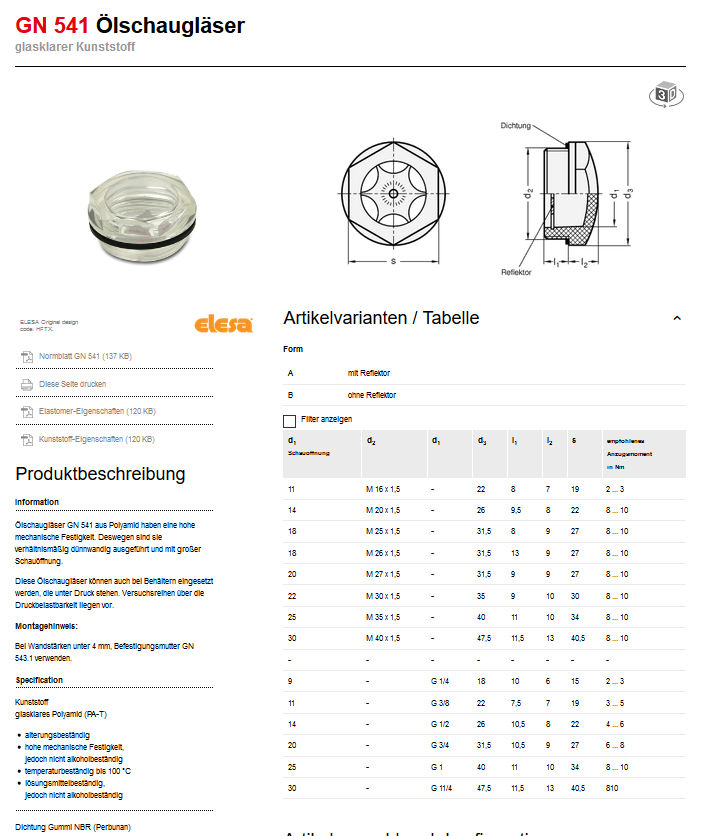
\includegraphics[width=1.1\textwidth,keepaspectratio]{figures/Oelschauglas.png}
	\caption{Datenblatt Ölschauglas \protect\cite{bib:www:schauglas}}
	%		\caption{Datenblatt Reibbelag\protect\ccite{bib:www:reibbelag}\protect\footnotemark}
	\label{fig:schauglas }
\end{figure}
\footnotetext{Vgl. [Gria] }

\newpage
\begin{figure}[H]
	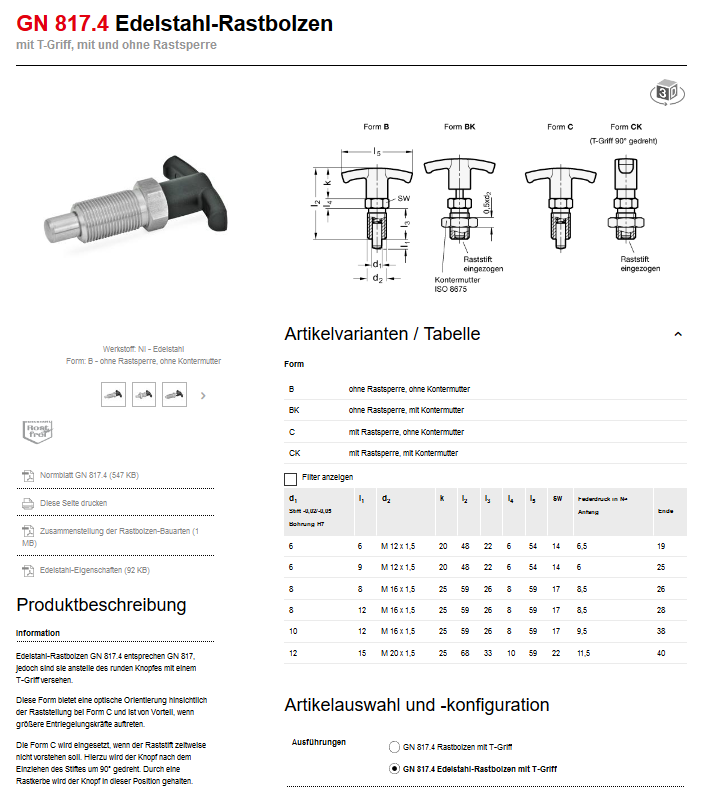
\includegraphics[width=1.1\textwidth,keepaspectratio]{figures/Rastbolzen.png}
	\caption{Datenblatt Arretierung Schaltung 1 \protect\cite{bib:www:rastbolzen}}
	%		\caption{Datenblatt Reibbelag\protect\ccite{bib:www:reibbelag}\protect\footnotemark}
	\label{fig:rastbolzen}
\end{figure}
\footnotetext{Vgl. [Grib] }

	\begin{figure}[H]
	\vspace{-2cm}
	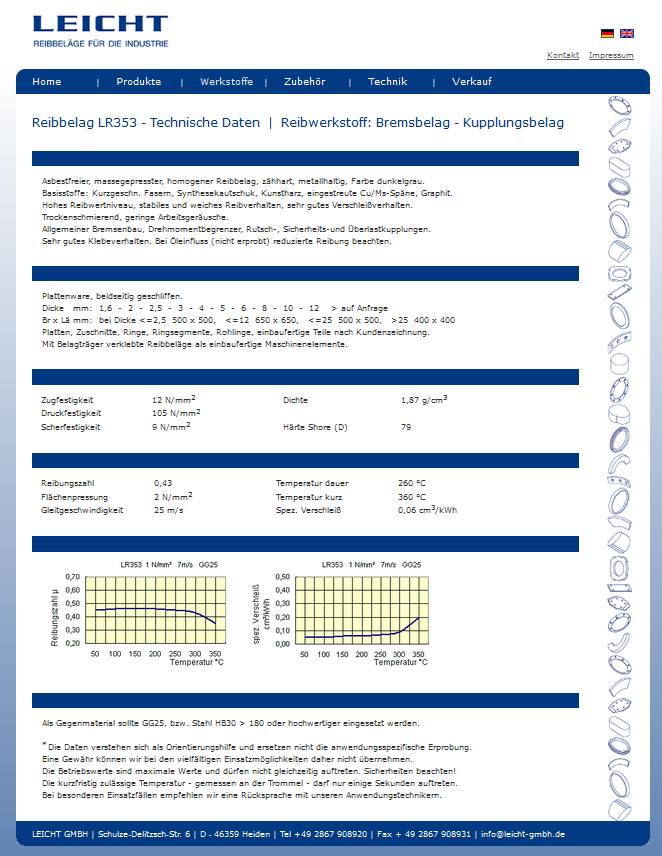
\includegraphics[width=1.0773\textwidth,keepaspectratio]{figures/Reibbelag.png}
	\caption{Datenblatt Reibbelag \protect\cite{bib:www:reibbelag}}
	%		\caption{Datenblatt Reibbelag\protect\ccite{bib:www:reibbelag}\protect\footnotemark}
	\label{fig:Reibbelag}
\end{figure}
\footnotetext{Vgl. [Gmb] }
	
	
	% Ende Hauptdokument
	
\end{document}